%********************************************%
%*       Generated from PreTeXt source      *%
%*       on 2021-05-15T13:52:35-04:00       *%
%*   A recent stable commit (2020-08-09):   *%
%* 98f21740783f166a773df4dc83cab5293ab63a4a *%
%*                                          *%
%*         https://pretextbook.org          *%
%*                                          *%
%********************************************%
%% We elect to always write snapshot output into <job>.dep file
\RequirePackage{snapshot}
\documentclass[oneside,10pt,]{book}
%% Custom Preamble Entries, early (use latex.preamble.early)
%% Default LaTeX packages
%%   1.  always employed (or nearly so) for some purpose, or
%%   2.  a stylewriter may assume their presence
\usepackage{geometry}
%% Some aspects of the preamble are conditional,
%% the LaTeX engine is one such determinant
\usepackage{ifthen}
%% etoolbox has a variety of modern conveniences
\usepackage{etoolbox}
\usepackage{ifxetex,ifluatex}
%% Raster graphics inclusion
\usepackage{graphicx}
%% Color support, xcolor package
%% Always loaded, for: add/delete text, author tools
%% Here, since tcolorbox loads tikz, and tikz loads xcolor
\PassOptionsToPackage{usenames,dvipsnames,svgnames,table}{xcolor}
\usepackage{xcolor}
%% begin: defined colors, via xcolor package, for styling
%% end: defined colors, via xcolor package, for styling
%% Colored boxes, and much more, though mostly styling
%% skins library provides "enhanced" skin, employing tikzpicture
%% boxes may be configured as "breakable" or "unbreakable"
%% "raster" controls grids of boxes, aka side-by-side
\usepackage{tcolorbox}
\tcbuselibrary{skins}
\tcbuselibrary{breakable}
\tcbuselibrary{raster}
%% We load some "stock" tcolorbox styles that we use a lot
%% Placement here is provisional, there will be some color work also
%% First, black on white, no border, transparent, but no assumption about titles
\tcbset{ bwminimalstyle/.style={size=minimal, boxrule=-0.3pt, frame empty,
colback=white, colbacktitle=white, coltitle=black, opacityfill=0.0} }
%% Second, bold title, run-in to text/paragraph/heading
%% Space afterwards will be controlled by environment,
%% independent of constructions of the tcb title
%% Places \blocktitlefont onto many block titles
\tcbset{ runintitlestyle/.style={fonttitle=\blocktitlefont\upshape\bfseries, attach title to upper} }
%% Spacing prior to each exercise, anywhere
\tcbset{ exercisespacingstyle/.style={before skip={1.5ex plus 0.5ex}} }
%% Spacing prior to each block
\tcbset{ blockspacingstyle/.style={before skip={2.0ex plus 0.5ex}} }
%% xparse allows the construction of more robust commands,
%% this is a necessity for isolating styling and behavior
%% The tcolorbox library of the same name loads the base library
\tcbuselibrary{xparse}
%% Hyperref should be here, but likes to be loaded late
%%
%% Inline math delimiters, \(, \), need to be robust
%% 2016-01-31:  latexrelease.sty  supersedes  fixltx2e.sty
%% If  latexrelease.sty  exists, bugfix is in kernel
%% If not, bugfix is in  fixltx2e.sty
%% See:  https://tug.org/TUGboat/tb36-3/tb114ltnews22.pdf
%% and read "Fewer fragile commands" in distribution's  latexchanges.pdf
\IfFileExists{latexrelease.sty}{}{\usepackage{fixltx2e}}
%% shorter subnumbers in some side-by-side require manipulations
\usepackage{xstring}
%% Footnote counters and part/chapter counters are manipulated
%% April 2018:  chngcntr  commands now integrated into the kernel,
%% but circa 2018/2019 the package would still try to redefine them,
%% so we need to do the work of loading conditionally for old kernels.
%% From version 1.1a,  chngcntr  should detect defintions made by LaTeX kernel.
\ifdefined\counterwithin
\else
    \usepackage{chngcntr}
\fi
%% Text height identically 9 inches, text width varies on point size
%% See Bringhurst 2.1.1 on measure for recommendations
%% 75 characters per line (count spaces, punctuation) is target
%% which is the upper limit of Bringhurst's recommendations
\geometry{letterpaper,total={340pt,9.0in}}
%% Custom Page Layout Adjustments (use latex.geometry)
%% This LaTeX file may be compiled with pdflatex, xelatex, or lualatex executables
%% LuaTeX is not explicitly supported, but we do accept additions from knowledgeable users
%% The conditional below provides  pdflatex  specific configuration last
%% begin: engine-specific capabilities
\ifthenelse{\boolean{xetex} \or \boolean{luatex}}{%
%% begin: xelatex and lualatex-specific default configuration
\ifxetex\usepackage{xltxtra}\fi
%% realscripts is the only part of xltxtra relevant to lualatex 
\ifluatex\usepackage{realscripts}\fi
%% end:   xelatex and lualatex-specific default configuration
}{
%% begin: pdflatex-specific default configuration
%% We assume a PreTeXt XML source file may have Unicode characters
%% and so we ask LaTeX to parse a UTF-8 encoded file
%% This may work well for accented characters in Western language,
%% but not with Greek, Asian languages, etc.
%% When this is not good enough, switch to the  xelatex  engine
%% where Unicode is better supported (encouraged, even)
\usepackage[utf8]{inputenc}
%% end: pdflatex-specific default configuration
}
%% end:   engine-specific capabilities
%%
%% Fonts.  Conditional on LaTex engine employed.
%% Default Text Font: The Latin Modern fonts are
%% "enhanced versions of the [original TeX] Computer Modern fonts."
%% We use them as the default text font for PreTeXt output.
%% Default Monospace font: Inconsolata (aka zi4)
%% Sponsored by TUG: http://levien.com/type/myfonts/inconsolata.html
%% Loaded for documents with intentional objects requiring monospace
%% See package documentation for excellent instructions
%% fontspec will work universally if we use filename to locate OTF files
%% Loads the "upquote" package as needed, so we don't have to
%% Upright quotes might come from the  textcomp  package, which we also use
%% We employ the shapely \ell to match Google Font version
%% pdflatex: "varl" package option produces shapely \ell
%% pdflatex: "var0" package option produces plain zero (not used)
%% pdflatex: "varqu" package option produces best upright quotes
%% xelatex,lualatex: add OTF StylisticSet 1 for shapely \ell
%% xelatex,lualatex: add OTF StylisticSet 2 for plain zero (not used)
%% xelatex,lualatex: add OTF StylisticSet 3 for upright quotes
%%
%% Automatic Font Control
%% Portions of a document, are, or may, be affected by defined commands
%% These are perhaps more flexible when using  xelatex  rather than  pdflatex
%% The following definitions are meant to be re-defined in a style, using \renewcommand
%% They are scoped when employed (in a TeX group), and so should not be defined with an argument
\newcommand{\divisionfont}{\relax}
\newcommand{\blocktitlefont}{\relax}
\newcommand{\contentsfont}{\relax}
\newcommand{\pagefont}{\relax}
\newcommand{\tabularfont}{\relax}
\newcommand{\xreffont}{\relax}
\newcommand{\titlepagefont}{\relax}
%%
\ifthenelse{\boolean{xetex} \or \boolean{luatex}}{%
%% begin: font setup and configuration for use with xelatex
%% Generally, xelatex is necessary for non-Western fonts
%% fontspec package provides extensive control of system fonts,
%% meaning *.otf (OpenType), and apparently *.ttf (TrueType)
%% that live *outside* your TeX/MF tree, and are controlled by your *system*
%% (it is possible that a TeX distribution will place fonts in a system location)
%%
%% The fontspec package is the best vehicle for using different fonts in  xelatex
%% So we load it always, no matter what a publisher or style might want
%%
\usepackage{fontspec}
%%
%% begin: xelatex main font ("font-xelatex-main" template)
%% Latin Modern Roman is the default font for xelatex and so is loaded with a TU encoding
%% *in the format* so we can't touch it, only perhaps adjust it later
%% in one of two ways (then known by NFSS names such as "lmr")
%% (1) via NFSS with font family names such as "lmr" and "lmss"
%% (2) via fontspec with commands like \setmainfont{Latin Modern Roman}
%% The latter requires the font to be known at the system-level by its font name,
%% but will give access to OTF font features through optional arguments
%% https://tex.stackexchange.com/questions/470008/
%% where-and-how-does-fontspec-sty-specify-the-default-font-latin-modern-roman
%% http://tex.stackexchange.com/questions/115321
%% /how-to-optimize-latin-modern-font-with-xelatex
%%
%% end:   xelatex main font ("font-xelatex-main" template)
%% begin: xelatex mono font ("font-xelatex-mono" template)
%% (conditional on non-trivial uses being present in source)
\IfFontExistsTF{Inconsolatazi4-Regular.otf}{}{\GenericError{}{The font "Inconsolatazi4-Regular.otf" requested by PreTeXt output is not available.  Either a file cannot be located in default locations via a filename, or a font is not known by its name as part of your system.}{Consult the PreTeXt Guide for help with LaTeX fonts.}{}}
\IfFontExistsTF{Inconsolatazi4-Bold.otf}{}{\GenericError{}{The font "Inconsolatazi4-Bold.otf" requested by PreTeXt output is not available.  Either a file cannot be located in default locations via a filename, or a font is not known by its name as part of your system.}{Consult the PreTeXt Guide for help with LaTeX fonts.}{}}
\usepackage{zi4}
\setmonofont[BoldFont=Inconsolatazi4-Bold.otf,StylisticSet={1,3}]{Inconsolatazi4-Regular.otf}
%% end:   xelatex mono font ("font-xelatex-mono" template)
%% begin: xelatex font adjustments ("font-xelatex-style" template)
%% end:   xelatex font adjustments ("font-xelatex-style" template)
%%
%% Extensive support for other languages
\usepackage{polyglossia}
%% Set main/default language based on pretext/@xml:lang value
%% document language code is "en-US", US English
%% usmax variant has extra hypenation
\setmainlanguage[variant=usmax]{english}
%% Enable secondary languages based on discovery of @xml:lang values
%% Enable fonts/scripts based on discovery of @xml:lang values
%% Western languages should be ably covered by Latin Modern Roman
%% end:   font setup and configuration for use with xelatex
}{%
%% begin: font setup and configuration for use with pdflatex
%% begin: pdflatex main font ("font-pdflatex-main" template)
\usepackage{lmodern}
\usepackage[T1]{fontenc}
%% end:   pdflatex main font ("font-pdflatex-main" template)
%% begin: pdflatex mono font ("font-pdflatex-mono" template)
%% (conditional on non-trivial uses being present in source)
\usepackage[varqu,varl]{inconsolata}
%% end:   pdflatex mono font ("font-pdflatex-mono" template)
%% begin: pdflatex font adjustments ("font-pdflatex-style" template)
%% end:   pdflatex font adjustments ("font-pdflatex-style" template)
%% end:   font setup and configuration for use with pdflatex
}
%% Micromanage spacing, etc.  The named "microtype-options"
%% template may be employed to fine-tune package behavior
\usepackage{microtype}
%% Symbols, align environment, commutative diagrams, bracket-matrix
\usepackage{amsmath}
\usepackage{amscd}
\usepackage{amssymb}
%% allow page breaks within display mathematics anywhere
%% level 4 is maximally permissive
%% this is exactly the opposite of AMSmath package philosophy
%% there are per-display, and per-equation options to control this
%% split, aligned, gathered, and alignedat are not affected
\allowdisplaybreaks[4]
%% allow more columns to a matrix
%% can make this even bigger by overriding with  latex.preamble.late  processing option
\setcounter{MaxMatrixCols}{30}
%%
%%
%% Division Titles, and Page Headers/Footers
%% titlesec package, loading "titleps" package cooperatively
%% See code comments about the necessity and purpose of "explicit" option.
%% The "newparttoc" option causes a consistent entry for parts in the ToC 
%% file, but it is only effective if there is a \titleformat for \part.
%% "pagestyles" loads the  titleps  package cooperatively.
\usepackage[explicit, newparttoc, pagestyles]{titlesec}
%% The companion titletoc package for the ToC.
\usepackage{titletoc}
%% Fixes a bug with transition from chapters to appendices in a "book"
%% See generating XSL code for more details about necessity
\newtitlemark{\chaptertitlename}
%% begin: customizations of page styles via the modal "titleps-style" template
%% Designed to use commands from the LaTeX "titleps" package
%% Plain pages should have the same font for page numbers
\renewpagestyle{plain}{%
\setfoot{}{\pagefont\thepage}{}%
}%
%% Single pages as in default LaTeX
\renewpagestyle{headings}{%
\sethead{\pagefont\slshape\MakeUppercase{\ifthechapter{\chaptertitlename\space\thechapter.\space}{}\chaptertitle}}{}{\pagefont\thepage}%
}%
\pagestyle{headings}
%% end: customizations of page styles via the modal "titleps-style" template
%%
%% Create globally-available macros to be provided for style writers
%% These are redefined for each occurence of each division
\newcommand{\divisionnameptx}{\relax}%
\newcommand{\titleptx}{\relax}%
\newcommand{\subtitleptx}{\relax}%
\newcommand{\shortitleptx}{\relax}%
\newcommand{\authorsptx}{\relax}%
\newcommand{\epigraphptx}{\relax}%
%% Create environments for possible occurences of each division
%% Environment for a PTX "preface" at the level of a LaTeX "chapter"
\NewDocumentEnvironment{preface}{mmmmmm}
{%
\renewcommand{\divisionnameptx}{Preface}%
\renewcommand{\titleptx}{#1}%
\renewcommand{\subtitleptx}{#2}%
\renewcommand{\shortitleptx}{#3}%
\renewcommand{\authorsptx}{#4}%
\renewcommand{\epigraphptx}{#5}%
\chapter*{#1}%
\addcontentsline{toc}{chapter}{#3}
\label{#6}%
}{}%
%% Environment for a PTX "part" at the level of a LaTeX "part"
\NewDocumentEnvironment{partptx}{mmmmmm}
{%
\renewcommand{\divisionnameptx}{Part}%
\renewcommand{\titleptx}{#1}%
\renewcommand{\subtitleptx}{#2}%
\renewcommand{\shortitleptx}{#3}%
\renewcommand{\authorsptx}{#4}%
\renewcommand{\epigraphptx}{#5}%
\part[{#3}]{#1}%
\label{#6}%
}{}%
%% Environment for a PTX "chapter" at the level of a LaTeX "chapter"
\NewDocumentEnvironment{chapterptx}{mmmmmm}
{%
\renewcommand{\divisionnameptx}{Chapter}%
\renewcommand{\titleptx}{#1}%
\renewcommand{\subtitleptx}{#2}%
\renewcommand{\shortitleptx}{#3}%
\renewcommand{\authorsptx}{#4}%
\renewcommand{\epigraphptx}{#5}%
\chapter[{#3}]{#1}%
\label{#6}%
}{}%
%% Environment for a PTX "section" at the level of a LaTeX "section"
\NewDocumentEnvironment{sectionptx}{mmmmmm}
{%
\renewcommand{\divisionnameptx}{Section}%
\renewcommand{\titleptx}{#1}%
\renewcommand{\subtitleptx}{#2}%
\renewcommand{\shortitleptx}{#3}%
\renewcommand{\authorsptx}{#4}%
\renewcommand{\epigraphptx}{#5}%
\section[{#3}]{#1}%
\label{#6}%
}{}%
%% Environment for a PTX "exercises" at the level of a LaTeX "subsection"
\NewDocumentEnvironment{exercises-subsection}{mmmmmm}
{%
\renewcommand{\divisionnameptx}{Exercises}%
\renewcommand{\titleptx}{#1}%
\renewcommand{\subtitleptx}{#2}%
\renewcommand{\shortitleptx}{#3}%
\renewcommand{\authorsptx}{#4}%
\renewcommand{\epigraphptx}{#5}%
\subsection[{#3}]{#1}%
\label{#6}%
}{}%
%% Environment for a PTX "exercises" at the level of a LaTeX "subsection"
\NewDocumentEnvironment{exercises-subsection-numberless}{mmmmmm}
{%
\renewcommand{\divisionnameptx}{Exercises}%
\renewcommand{\titleptx}{#1}%
\renewcommand{\subtitleptx}{#2}%
\renewcommand{\shortitleptx}{#3}%
\renewcommand{\authorsptx}{#4}%
\renewcommand{\epigraphptx}{#5}%
\subsection*{#1}%
\addcontentsline{toc}{subsection}{#3}
\label{#6}%
}{}%
%% Environment for a PTX "reading-questions" at the level of a LaTeX "subsection"
\NewDocumentEnvironment{reading-questions-subsection}{mmmmmm}
{%
\renewcommand{\divisionnameptx}{Reading Questions}%
\renewcommand{\titleptx}{#1}%
\renewcommand{\subtitleptx}{#2}%
\renewcommand{\shortitleptx}{#3}%
\renewcommand{\authorsptx}{#4}%
\renewcommand{\epigraphptx}{#5}%
\subsection[{#3}]{#1}%
\label{#6}%
}{}%
%% Environment for a PTX "reading-questions" at the level of a LaTeX "subsection"
\NewDocumentEnvironment{reading-questions-subsection-numberless}{mmmmmm}
{%
\renewcommand{\divisionnameptx}{Reading Questions}%
\renewcommand{\titleptx}{#1}%
\renewcommand{\subtitleptx}{#2}%
\renewcommand{\shortitleptx}{#3}%
\renewcommand{\authorsptx}{#4}%
\renewcommand{\epigraphptx}{#5}%
\subsection*{#1}%
\addcontentsline{toc}{subsection}{#3}
\label{#6}%
}{}%
%% Environment for a PTX "references" at the level of a LaTeX "chapter"
\NewDocumentEnvironment{references-chapter}{mmmmmm}
{%
\renewcommand{\divisionnameptx}{References}%
\renewcommand{\titleptx}{#1}%
\renewcommand{\subtitleptx}{#2}%
\renewcommand{\shortitleptx}{#3}%
\renewcommand{\authorsptx}{#4}%
\renewcommand{\epigraphptx}{#5}%
\chapter[{#3}]{#1}%
\label{#6}%
}{}%
%% Environment for a PTX "references" at the level of a LaTeX "chapter"
\NewDocumentEnvironment{references-chapter-numberless}{mmmmmm}
{%
\renewcommand{\divisionnameptx}{References}%
\renewcommand{\titleptx}{#1}%
\renewcommand{\subtitleptx}{#2}%
\renewcommand{\shortitleptx}{#3}%
\renewcommand{\authorsptx}{#4}%
\renewcommand{\epigraphptx}{#5}%
\chapter*{#1}%
\addcontentsline{toc}{chapter}{#3}
\label{#6}%
}{}%
%% Environment for a PTX "index" at the level of a LaTeX "chapter"
\NewDocumentEnvironment{indexptx}{mmmmmm}
{%
\renewcommand{\divisionnameptx}{Index}%
\renewcommand{\titleptx}{#1}%
\renewcommand{\subtitleptx}{#2}%
\renewcommand{\shortitleptx}{#3}%
\renewcommand{\authorsptx}{#4}%
\renewcommand{\epigraphptx}{#5}%
\chapter*{#1}%
\addcontentsline{toc}{chapter}{#3}
\label{#6}%
}{}%
%%
%% Styles for six traditional LaTeX divisions
\titleformat{\part}[display]
{\divisionfont\Huge\bfseries\centering}{\divisionnameptx\space\thepart}{30pt}{\Huge#1}
[{\Large\centering\authorsptx}]
\titleformat{\chapter}[display]
{\divisionfont\huge\bfseries}{\divisionnameptx\space\thechapter}{20pt}{\Huge#1}
[{\Large\authorsptx}]
\titleformat{name=\chapter,numberless}[display]
{\divisionfont\huge\bfseries}{}{0pt}{#1}
[{\Large\authorsptx}]
\titlespacing*{\chapter}{0pt}{50pt}{40pt}
\titleformat{\section}[hang]
{\divisionfont\Large\bfseries}{\thesection}{1ex}{#1}
[{\large\authorsptx}]
\titleformat{name=\section,numberless}[block]
{\divisionfont\Large\bfseries}{}{0pt}{#1}
[{\large\authorsptx}]
\titlespacing*{\section}{0pt}{3.5ex plus 1ex minus .2ex}{2.3ex plus .2ex}
\titleformat{\subsection}[hang]
{\divisionfont\large\bfseries}{\thesubsection}{1ex}{#1}
[{\normalsize\authorsptx}]
\titleformat{name=\subsection,numberless}[block]
{\divisionfont\large\bfseries}{}{0pt}{#1}
[{\normalsize\authorsptx}]
\titlespacing*{\subsection}{0pt}{3.25ex plus 1ex minus .2ex}{1.5ex plus .2ex}
\titleformat{\subsubsection}[hang]
{\divisionfont\normalsize\bfseries}{\thesubsubsection}{1em}{#1}
[{\small\authorsptx}]
\titleformat{name=\subsubsection,numberless}[block]
{\divisionfont\normalsize\bfseries}{}{0pt}{#1}
[{\normalsize\authorsptx}]
\titlespacing*{\subsubsection}{0pt}{3.25ex plus 1ex minus .2ex}{1.5ex plus .2ex}
\titleformat{\paragraph}[hang]
{\divisionfont\normalsize\bfseries}{\theparagraph}{1em}{#1}
[{\small\authorsptx}]
\titleformat{name=\paragraph,numberless}[block]
{\divisionfont\normalsize\bfseries}{}{0pt}{#1}
[{\normalsize\authorsptx}]
\titlespacing*{\paragraph}{0pt}{3.25ex plus 1ex minus .2ex}{1.5em}
%%
%% Styles for five traditional LaTeX divisions
\titlecontents{part}%
[0pt]{\contentsmargin{0em}\addvspace{1pc}\contentsfont\bfseries}%
{\Large\thecontentslabel\enspace}{\Large}%
{}%
[\addvspace{.5pc}]%
\titlecontents{chapter}%
[0pt]{\contentsmargin{0em}\addvspace{1pc}\contentsfont\bfseries}%
{\large\thecontentslabel\enspace}{\large}%
{\hfill\bfseries\thecontentspage}%
[\addvspace{.5pc}]%
\dottedcontents{section}[3.8em]{\contentsfont}{2.3em}{1pc}%
\dottedcontents{subsection}[6.1em]{\contentsfont}{3.2em}{1pc}%
\dottedcontents{subsubsection}[9.3em]{\contentsfont}{4.3em}{1pc}%
%%
%% Begin: Semantic Macros
%% To preserve meaning in a LaTeX file
%%
%% \mono macro for content of "c", "cd", "tag", etc elements
%% Also used automatically in other constructions
%% Simply an alias for \texttt
%% Always defined, even if there is no need, or if a specific tt font is not loaded
\newcommand{\mono}[1]{\texttt{#1}}
%%
%% Following semantic macros are only defined here if their
%% use is required only in this specific document
%%
%% Used for inline definitions of terms
\newcommand{\terminology}[1]{\textbf{#1}}
%% End: Semantic Macros
%% Divisional exercises (and worksheet) as LaTeX environments
%% Third argument is option for extra workspace in worksheets
%% Hanging indent occupies a 5ex width slot prior to left margin
%% Experimentally this seems just barely sufficient for a bold "888."
%% Division exercises, not in exercise group
\tcbset{ divisionexercisestyle/.style={bwminimalstyle, runintitlestyle, exercisespacingstyle, left=5ex, breakable, parbox=false } }
\newtcolorbox{divisionexercise}[4]{divisionexercisestyle, before title={\hspace{-5ex}\makebox[5ex][l]{#1.}}, title={\notblank{#2}{#2\space}{}}, phantom={\hypertarget{#4}{}}, after={\notblank{#3}{\newline\rule{\workspacestrutwidth}{#3}\newline}{}}}
%% Division exercises, in exercise group, no columns
\tcbset{ divisionexerciseegstyle/.style={bwminimalstyle, runintitlestyle, exercisespacingstyle, left=5ex, left skip=\egindent, breakable, parbox=false } }
\newtcolorbox{divisionexerciseeg}[4]{divisionexerciseegstyle, before title={\hspace{-5ex}\makebox[5ex][l]{#1.}}, title={\notblank{#2}{#2\space}{}}, phantom={\hypertarget{#4}{}}, after={\notblank{#3}{\newline\rule{\workspacestrutwidth}{#3}\newline}{}}}
%% Localize LaTeX supplied names (possibly none)
\renewcommand*{\partname}{Part}
\renewcommand*{\chaptername}{Chapter}
%% Equation Numbering
%% Controlled by  numbering.equations.level  processing parameter
%% No adjustment here implies document-wide numbering
\numberwithin{equation}{section}
%% "tcolorbox" environment for a single image, occupying entire \linewidth
%% arguments are left-margin, width, right-margin, as multiples of
%% \linewidth, and are guaranteed to be positive and sum to 1.0
\tcbset{ imagestyle/.style={bwminimalstyle} }
\NewTColorBox{image}{mmm}{imagestyle,left skip=#1\linewidth,width=#2\linewidth}
%% For improved tables
\usepackage{array}
%% Some extra height on each row is desirable, especially with horizontal rules
%% Increment determined experimentally
\setlength{\extrarowheight}{0.2ex}
%% Define variable thickness horizontal rules, full and partial
%% Thicknesses are 0.03, 0.05, 0.08 in the  booktabs  package
\newcommand{\hrulethin}  {\noalign{\hrule height 0.04em}}
\newcommand{\hrulemedium}{\noalign{\hrule height 0.07em}}
\newcommand{\hrulethick} {\noalign{\hrule height 0.11em}}
%% We preserve a copy of the \setlength package before other
%% packages (extpfeil) get a chance to load packages that redefine it
\let\oldsetlength\setlength
\newlength{\Oldarrayrulewidth}
\newcommand{\crulethin}[1]%
{\noalign{\global\oldsetlength{\Oldarrayrulewidth}{\arrayrulewidth}}%
\noalign{\global\oldsetlength{\arrayrulewidth}{0.04em}}\cline{#1}%
\noalign{\global\oldsetlength{\arrayrulewidth}{\Oldarrayrulewidth}}}%
\newcommand{\crulemedium}[1]%
{\noalign{\global\oldsetlength{\Oldarrayrulewidth}{\arrayrulewidth}}%
\noalign{\global\oldsetlength{\arrayrulewidth}{0.07em}}\cline{#1}%
\noalign{\global\oldsetlength{\arrayrulewidth}{\Oldarrayrulewidth}}}
\newcommand{\crulethick}[1]%
{\noalign{\global\oldsetlength{\Oldarrayrulewidth}{\arrayrulewidth}}%
\noalign{\global\oldsetlength{\arrayrulewidth}{0.11em}}\cline{#1}%
\noalign{\global\oldsetlength{\arrayrulewidth}{\Oldarrayrulewidth}}}
%% Single letter column specifiers defined via array package
\newcolumntype{A}{!{\vrule width 0.04em}}
\newcolumntype{B}{!{\vrule width 0.07em}}
\newcolumntype{C}{!{\vrule width 0.11em}}
%% tcolorbox to place tabular outside of a sidebyside
\tcbset{ tabularboxstyle/.style={bwminimalstyle,} }
\newtcolorbox{tabularbox}[3]{tabularboxstyle, left skip=#1\linewidth, width=#2\linewidth,}
%% Program listing support: for listings, programs, consoles, and Sage code
\ifthenelse{\boolean{xetex} \or \boolean{luatex}}%
  {\tcbuselibrary{listings}}%
  {\tcbuselibrary{listingsutf8}}%
%% We define the listings font style to be the default "ttfamily"
%% To fix hyphens/dashes rendered in PDF as fancy minus signs by listing
%% http://tex.stackexchange.com/questions/33185/listings-package-changes-hyphens-to-minus-signs
\makeatletter
\lst@CCPutMacro\lst@ProcessOther {"2D}{\lst@ttfamily{-{}}{-{}}}
\@empty\z@\@empty
\makeatother
%% We define a null language, free of any formatting or style
%% for use when a language is not supported, or pseudo-code, or consoles
%% Not necessary for Sage code, so in limited cases included unnecessarily
\lstdefinelanguage{none}{identifierstyle=,commentstyle=,stringstyle=,keywordstyle=}
\ifthenelse{\boolean{xetex}}{}{%
%% begin: pdflatex-specific listings configuration
%% translate U+0080 - U+00F0 to their textmode LaTeX equivalents
%% Data originally from https://www.w3.org/Math/characters/unicode.xml, 2016-07-23
%% Lines marked in XSL with "$" were converted from mathmode to textmode
\lstset{extendedchars=true}
\lstset{literate={ }{{~}}{1}{¡}{{\textexclamdown }}{1}{¢}{{\textcent }}{1}{£}{{\textsterling }}{1}{¤}{{\textcurrency }}{1}{¥}{{\textyen }}{1}{¦}{{\textbrokenbar }}{1}{§}{{\textsection }}{1}{¨}{{\textasciidieresis }}{1}{©}{{\textcopyright }}{1}{ª}{{\textordfeminine }}{1}{«}{{\guillemotleft }}{1}{¬}{{\textlnot }}{1}{­}{{\-}}{1}{®}{{\textregistered }}{1}{¯}{{\textasciimacron }}{1}{°}{{\textdegree }}{1}{±}{{\textpm }}{1}{²}{{\texttwosuperior }}{1}{³}{{\textthreesuperior }}{1}{´}{{\textasciiacute }}{1}{µ}{{\textmu }}{1}{¶}{{\textparagraph }}{1}{·}{{\textperiodcentered }}{1}{¸}{{\c{}}}{1}{¹}{{\textonesuperior }}{1}{º}{{\textordmasculine }}{1}{»}{{\guillemotright }}{1}{¼}{{\textonequarter }}{1}{½}{{\textonehalf }}{1}{¾}{{\textthreequarters }}{1}{¿}{{\textquestiondown }}{1}{À}{{\`{A}}}{1}{Á}{{\'{A}}}{1}{Â}{{\^{A}}}{1}{Ã}{{\~{A}}}{1}{Ä}{{\"{A}}}{1}{Å}{{\AA }}{1}{Æ}{{\AE }}{1}{Ç}{{\c{C}}}{1}{È}{{\`{E}}}{1}{É}{{\'{E}}}{1}{Ê}{{\^{E}}}{1}{Ë}{{\"{E}}}{1}{Ì}{{\`{I}}}{1}{Í}{{\'{I}}}{1}{Î}{{\^{I}}}{1}{Ï}{{\"{I}}}{1}{Ð}{{\DH }}{1}{Ñ}{{\~{N}}}{1}{Ò}{{\`{O}}}{1}{Ó}{{\'{O}}}{1}{Ô}{{\^{O}}}{1}{Õ}{{\~{O}}}{1}{Ö}{{\"{O}}}{1}{×}{{\texttimes }}{1}{Ø}{{\O }}{1}{Ù}{{\`{U}}}{1}{Ú}{{\'{U}}}{1}{Û}{{\^{U}}}{1}{Ü}{{\"{U}}}{1}{Ý}{{\'{Y}}}{1}{Þ}{{\TH }}{1}{ß}{{\ss }}{1}{à}{{\`{a}}}{1}{á}{{\'{a}}}{1}{â}{{\^{a}}}{1}{ã}{{\~{a}}}{1}{ä}{{\"{a}}}{1}{å}{{\aa }}{1}{æ}{{\ae }}{1}{ç}{{\c{c}}}{1}{è}{{\`{e}}}{1}{é}{{\'{e}}}{1}{ê}{{\^{e}}}{1}{ë}{{\"{e}}}{1}{ì}{{\`{\i}}}{1}{í}{{\'{\i}}}{1}{î}{{\^{\i}}}{1}{ï}{{\"{\i}}}{1}{ð}{{\dh }}{1}{ñ}{{\~{n}}}{1}{ò}{{\`{o}}}{1}{ó}{{\'{o}}}{1}{ô}{{\^{o}}}{1}{õ}{{\~{o}}}{1}{ö}{{\"{o}}}{1}{÷}{{\textdiv }}{1}{ø}{{\o }}{1}{ù}{{\`{u}}}{1}{ú}{{\'{u}}}{1}{û}{{\^{u}}}{1}{ü}{{\"{u}}}{1}{ý}{{\'{y}}}{1}{þ}{{\th }}{1}{ÿ}{{\"{y}}}{1}}
%% end: pdflatex-specific listings configuration
}
%% End of generic listing adjustments
%% The listings package as tcolorbox for Sage code
%% We do as much styling as possible with tcolorbox, not listings
%% Sage's blue is 50%, we go way lighter (blue!05 would also work)
%% Note that we defuse listings' default "aboveskip" and "belowskip"
\definecolor{sageblue}{rgb}{0.95,0.95,1}
\tcbset{ sagestyle/.style={left=0pt, right=0pt, top=0ex, bottom=0ex, middle=0pt, toptitle=0pt, bottomtitle=0pt,
boxsep=4pt, listing only, fontupper=\small\ttfamily,
breakable, parbox=false, 
listing options={language=Python,breaklines=true,breakatwhitespace=true, extendedchars=true, aboveskip=0pt, belowskip=0pt}} }
\newtcblisting{sageinput}{sagestyle, colback=sageblue, sharp corners, boxrule=0.5pt, toprule at break=-0.3pt, bottomrule at break=-0.3pt, }
\newtcblisting{sageoutput}{sagestyle, colback=white, colframe=white, frame empty, before skip=0pt, after skip=0pt, }
%% Fancy Verbatim for consoles, preformatted, code display, literate programming
\usepackage{fancyvrb}
%% code display (cd), by analogy with math display (md)
%% savebox, lrbox, etc to achieve centering
\newsavebox{\codedisplaybox}
\newenvironment{codedisplay}
{\VerbatimEnvironment\begin{center}\begin{lrbox}{\codedisplaybox}\begin{BVerbatim}}
{\end{BVerbatim}\end{lrbox}\usebox{\codedisplaybox}\end{center}}
%% Multiple column, column-major lists
\usepackage{multicol}
%% More flexible list management, esp. for references
%% But also for specifying labels (i.e. custom order) on nested lists
\usepackage{enumitem}
%% Lists of references in their own section, maximum depth 1
\newlist{referencelist}{description}{4}
\setlist[referencelist]{leftmargin=!,labelwidth=!,labelsep=0ex,itemsep=1.0ex,topsep=1.0ex,partopsep=0pt,parsep=0pt}
%% Indented groups of "exercise" within an "exercises" division
%% Lengths control the indentation (always) and gaps (multi-column)
\newlength{\egindent}\setlength{\egindent}{0.05\linewidth}
\newlength{\exggap}\setlength{\exggap}{0.05\linewidth}
%% Thin "xparse" environments will represent the entire exercise
%% group, in the case when it does not hold multiple columns.
\NewDocumentEnvironment{exercisegroup}{}
{}{}
%% Support for index creation
%% imakeidx package does not require extra pass (as with makeidx)
%% Title of the "Index" section set via a keyword
%% Language support for the "see" and "see also" phrases
\usepackage{imakeidx}
\makeindex[title=Index, intoc=true]
\renewcommand{\seename}{See}
\renewcommand{\alsoname}{See also}
%% Package for tables spanning several pages
\usepackage{longtable}
%% hyperref driver does not need to be specified, it will be detected
%% Footnote marks in tcolorbox have broken linking under
%% hyperref, so it is necessary to turn off all linking
%% It *must* be given as a package option, not with \hypersetup
\usepackage[hyperfootnotes=false]{hyperref}
%% configure hyperref's  \url  to match listings' inline verbatim
\renewcommand\UrlFont{\small\ttfamily}
%% Hyperlinking active in electronic PDFs, all links solid and blue
\hypersetup{colorlinks=true,linkcolor=blue,citecolor=blue,filecolor=blue,urlcolor=blue}
\hypersetup{pdftitle={Active Applied Discrete Structures}}
%% If you manually remove hyperref, leave in this next command
%% This will allow LaTeX compilation, employing this no-op command
\providecommand\phantomsection{}
%% Division Numbering: Chapters, Sections, Subsections, etc
%% Division numbers may be turned off at some level ("depth")
%% A section *always* has depth 1, contrary to us counting from the document root
%% The latex default is 3.  If a larger number is present here, then
%% removing this command may make some cross-references ambiguous
%% The precursor variable $numbering-maxlevel is checked for consistency in the common XSL file
\setcounter{secnumdepth}{3}
%%
%% AMS "proof" environment is no longer used, but we leave previously
%% implemented \qedhere in place, should the LaTeX be recycled
\newcommand{\qedhere}{\relax}
%%
%% A faux tcolorbox whose only purpose is to provide common numbering
%% facilities for most blocks (possibly not projects, 2D displays)
%% Controlled by  numbering.theorems.level  processing parameter
\newtcolorbox[auto counter, number within=section]{block}{}
%%
%% This document is set to number PROJECT-LIKE on a separate numbering scheme
%% So, a faux tcolorbox whose only purpose is to provide this numbering
%% Controlled by  numbering.projects.level  processing parameter
\newtcolorbox[auto counter, number within=section]{project-distinct}{}
%% A faux tcolorbox whose only purpose is to provide common numbering
%% facilities for 2D displays which are subnumbered as part of a "sidebyside"
\makeatletter
\newtcolorbox[auto counter, number within=tcb@cnt@block, number freestyle={\noexpand\thetcb@cnt@block(\noexpand\alph{\tcbcounter})}]{subdisplay}{}
\makeatother
%%
%% tcolorbox, with styles, for THEOREM-LIKE
%%
%% theorem: fairly simple numbered block/structure
\tcbset{ theoremstyle/.style={bwminimalstyle, runintitlestyle, blockspacingstyle, after title={\space}, } }
\newtcolorbox[use counter from=block]{theorem}[3]{title={{Theorem~\thetcbcounter\notblank{#1#2}{\space}{}\notblank{#1}{\space#1}{}\notblank{#2}{\space(#2)}{}}}, phantomlabel={#3}, breakable, parbox=false, after={\par}, fontupper=\itshape, theoremstyle, }
%%
%% tcolorbox, with styles, for DEFINITION-LIKE
%%
%% definition: fairly simple numbered block/structure
\tcbset{ definitionstyle/.style={bwminimalstyle, runintitlestyle, blockspacingstyle, after title={\space}, after upper={\space\space\hspace*{\stretch{1}}\(\lozenge\)}, } }
\newtcolorbox[use counter from=block]{definition}[2]{title={{Definition~\thetcbcounter\notblank{#1}{\space\space#1}{}}}, phantomlabel={#2}, breakable, parbox=false, after={\par}, definitionstyle, }
%%
%% tcolorbox, with styles, for REMARK-LIKE
%%
%% note: fairly simple numbered block/structure
\tcbset{ notestyle/.style={bwminimalstyle, runintitlestyle, blockspacingstyle, after title={\space}, } }
\newtcolorbox[use counter from=block]{note}[2]{title={{Note~\thetcbcounter\notblank{#1}{\space\space#1}{}}}, phantomlabel={#2}, breakable, parbox=false, after={\par}, notestyle, }
%%
%% tcolorbox, with styles, for EXAMPLE-LIKE
%%
%% question: fairly simple numbered block/structure
\tcbset{ questionstyle/.style={bwminimalstyle, runintitlestyle, blockspacingstyle, after title={\space}, after upper={\space\space\hspace*{\stretch{1}}\(\square\)}, } }
\newtcolorbox[use counter from=block]{question}[2]{title={{Question~\thetcbcounter\notblank{#1}{\space\space#1}{}}}, phantomlabel={#2}, breakable, parbox=false, after={\par}, questionstyle, }
%%
%% tcolorbox, with styles, for FIGURE-LIKE
%%
%% figureptx: 2-D display structure
\tcbset{ figureptxstyle/.style={bwminimalstyle, middle=1ex, blockspacingstyle, fontlower=\blocktitlefont} }
\newtcolorbox[use counter from=block]{figureptx}[3]{lower separated=false, before lower={{\textbf{Figure~\thetcbcounter}\space#1}}, phantomlabel={#2}, unbreakable, parbox=false, figureptxstyle, }
%% tableptx: 2-D display structure
\tcbset{ tableptxstyle/.style={bwminimalstyle, middle=1ex, blockspacingstyle, coltitle=black, bottomtitle=2ex, titlerule=-0.3pt, fonttitle=\blocktitlefont} }
\newtcolorbox[use counter from=block]{tableptx}[3]{title={{\textbf{Table~\thetcbcounter}\space#1}}, phantomlabel={#2}, unbreakable, parbox=false, tableptxstyle, }
%%
%% xparse environments for introductions and conclusions of divisions
%%
%% introduction: in a structured division
\NewDocumentEnvironment{introduction}{m}
{\notblank{#1}{\noindent\textbf{#1}\space}{}}{\par\medskip}
%% conclusion: in a structured division
\NewDocumentEnvironment{conclusion}{m}
{\par\medskip\noindent\notblank{#1}{\textbf{#1}\space}{}}{}
%%
%% tcolorbox, with styles, for miscellaneous environments
%%
%% paragraphs: the terminal, pseudo-division
%% We use the lowest LaTeX traditional division
\titleformat{\subparagraph}[runin]{\normalfont\normalsize\bfseries}{\thesubparagraph}{1em}{#1}
\titlespacing*{\subparagraph}{0pt}{3.25ex plus 1ex minus .2ex}{1em}
\NewDocumentEnvironment{paragraphs}{mm}
{\subparagraph*{#1}\hypertarget{#2}{}}{}
%% Graphics Preamble Entries
    \usepackage{amsmath}
    \usepackage{tikz}
\usepackage{tkz-graph}
\usepackage{tkz-euclide}
\usepackage{chemfig}
\usetikzlibrary{patterns}
\usetikzlibrary{positioning}
\usetikzlibrary{matrix,arrows}
\usetikzlibrary{calc}
\usetikzlibrary{shapes}
\usetikzlibrary{through,intersections,decorations,shadows,fadings}
%% If tikz has been loaded, replace ampersand with \amp macro
%% tcolorbox styles for sidebyside layout
\tcbset{ sbsstyle/.style={raster before skip=2.0ex, raster equal height=rows, raster force size=false} }
\tcbset{ sbspanelstyle/.style={bwminimalstyle, fonttitle=\blocktitlefont} }
%% Enviroments for side-by-side and components
%% Necessary to use \NewTColorBox for boxes of the panels
%% "newfloat" environment to squash page-breaks within a single sidebyside
%% "xparse" environment for entire sidebyside
\NewDocumentEnvironment{sidebyside}{mmmm}
  {\begin{tcbraster}
    [sbsstyle,raster columns=#1,
    raster left skip=#2\linewidth,raster right skip=#3\linewidth,raster column skip=#4\linewidth]}
  {\end{tcbraster}}
%% "tcolorbox" environment for a panel of sidebyside
\NewTColorBox{sbspanel}{mO{top}}{sbspanelstyle,width=#1\linewidth,valign=#2}
%% extpfeil package for certain extensible arrows,
%% as also provided by MathJax extension of the same name
%% NB: this package loads mtools, which loads calc, which redefines
%%     \setlength, so it can be removed if it seems to be in the 
%%     way and your math does not use:
%%     
%%     \xtwoheadrightarrow, \xtwoheadleftarrow, \xmapsto, \xlongequal, \xtofrom
%%     
%%     we have had to be extra careful with variable thickness
%%     lines in tables, and so also load this package late
\usepackage{extpfeil}
%% Custom Preamble Entries, late (use latex.preamble.late)
%% Begin: Author-provided packages
%% (From  docinfo/latex-preamble/package  elements)
%% End: Author-provided packages
%% Begin: Author-provided macros
%% (From  docinfo/macros  element)
%% Plus three from MBX for XML characters
\usepackage[utf8]{inputenc}
\newcommand{\apple}{\text{🍎}}
\newcommand{\ap}{\apple}
\newcommand{\banana}{\text{🍌}}
\newcommand{\ba}{\banana}
\newcommand{\pear}{\text{🍐}}
\newcommand{\pe}{\pear}
\newcommand{\identity}{\mathrm{id}}
\newcommand{\notdivide}{{\not{\mid}}}
\newcommand{\notsubset}{\not\subset}
\newcommand{\lcm}{\operatorname{lcm}}
\newcommand{\gf}{\operatorname{GF}}
\newcommand{\inn}{\operatorname{Inn}}
\newcommand{\aut}{\operatorname{Aut}}
\newcommand{\Hom}{\operatorname{Hom}}
\newcommand{\cis}{\operatorname{cis}}
\newcommand{\chr}{\operatorname{char}}
\newcommand{\Null}{\operatorname{Null}}
\renewcommand{\vec}[1]{\mathbf{#1}}
\newcommand{\pow}{\mathcal P}
\newcommand{\inv}{^{-1}}
\newcommand{\st}{|}
\renewcommand{\iff}{\leftrightarrow}
\newcommand{\Iff}{\Leftrightarrow}
\newcommand{\imp}{\rightarrow}
\newcommand{\Imp}{\Rightarrow}
\newcommand{\isom}{\cong}

\newcommand{\card}[1]{\left| #1 \right|}
\newcommand{\twoline}[2]{\begin{pmatrix}#1 \\ #2 \end{pmatrix}}
\newcommand{\vtx}[2]{node[fill,circle,inner sep=0pt, minimum size=4pt,label=#1:#2]{}}
\newcommand{\va}[1]{\vtx{above}{#1}}
\newcommand{\vb}[1]{\vtx{below}{#1}}
\newcommand{\vr}[1]{\vtx{right}{#1}}
\newcommand{\vl}[1]{\vtx{left}{#1}}
\renewcommand{\v}{\vtx{above}{}}
\newcommand{\lt}{<}
\newcommand{\gt}{>}
\newcommand{\amp}{&}
%% End: Author-provided macros
\begin{document}
\frontmatter
%% begin: half-title
\thispagestyle{empty}
{\titlepagefont\centering
\vspace*{0.28\textheight}
{\Huge Active Applied Discrete Structures}\\}
\clearpage
%% end:   half-title
%% begin: title page
%% Inspired by Peter Wilson's "titleDB" in "titlepages" CTAN package
\thispagestyle{empty}
{\titlepagefont\centering
\vspace*{0.14\textheight}
%% Target for xref to top-level element is ToC
\addtocontents{toc}{\protect\hypertarget{x:book:active-ads}{}}
{\Huge Active Applied Discrete Structures}\\[3\baselineskip]
{\Large Ken Levasseur}\\[0.5\baselineskip]
{\Large University of Massachusetts Lowell}\\[3\baselineskip]
{\Large May 15, 2021}\\}
\clearpage
%% end:   title page
%% begin: copyright-page
\thispagestyle{empty}
\hypertarget{g:colophon:idm218170784816}{}\vspace*{\stretch{2}}
\noindent{\bfseries Edition}: version 0.1\par\medskip
\noindent{\bfseries Website}: \href{http:\slash{}\slash{}discretemath.org}{discretemath.org}\par\medskip
\noindent\textcopyright{}2020\quad{}Ken Levasseur\\[0.5\baselineskip]
Active Applied Discrete Structures by Kenneth Levasseur is licensed under a Creative Commons Attribution-NonCommercial-ShareAlike 3.0 United States License. You are free to Share: copy and redistribute the material in any medium or format; Adapt: remix, transform, and build upon the material. You may not use the material for commercial purposes.  The licensor cannot revoke these freedoms as long as you follow the license terms.\par\medskip
\vspace*{\stretch{1}}
\null\clearpage
%% end:   copyright-page
%
%
\typeout{************************************************}
\typeout{Preface  Preface}
\typeout{************************************************}
%
\begin{preface}{Preface}{}{Preface}{}{}{x:preface:active-ads-preface}
\begin{paragraphs}{Introduction.}{g:paragraphs:idm218170779456}%
\emph{Active Applied Discrete Structures} is designed for use in a flipped class using \emph{Applied Discrete Structures}. Each chapter, designed for a 75 minute class period.  There are two parts that correspond with a two semester sequence, \emph{Part 1 - Fundamentals}, and \emph{Part 2 - Structures}.%
\end{paragraphs}%
\begin{paragraphs}{Usage.}{g:paragraphs:idm218170778256}%
The class format that is presumed is for the instructor to assign students to read materials that will be covered in class \(n\) in time for students to submit a short assignment by the beginning of class \(n-1\). Then, at the time of class \(n\), they work on more challenging problems in groups of 4-6 students.%
\par
A tricky thing about this format is getting started. On class 1 of the first semester, no prior reading can be expected. The binary representation of positive integers is discussed. This is mostly done through group work. The assumption is that since most students in the class are computer science majors, they have some familiarity with the topic and can help  other students with the problems. Class 2 is also a bit of a rush. I ask students to do reading for that class and get responses back to me a couple of days before the second class. They are also asked to prepare for Class 3 and get responses to me by Class 2.   Fortunately, the material in Chapter 1 isn't too difficult.  The rest of the semester proceeds as described above. In the second semester, the first class is taken up by reviewing the most important concepts from the first semester through sequence of problems. Another quick turn-around in the reading for Class 2 is needed to get into the flow.  After that the second semester proceeds the same as the first.%
\end{paragraphs}%
\begin{paragraphs}{Contents of the Chapters.}{g:paragraphs:idm218170773824}%
Each chapter has two or three sections.  Each chapter except the first has a reading section that contains instructions to student prior the class period. Generally, this is to read one or more sections of the text, respond to a ``Response Question'' and do a few basic problems associated with the reading.  The Response Questions tend to be more tangential to the content and often connect the mathematics to computer science.%
\par
The second section is always a series of problems to be worked on during the class. For students' convenience, some chapters have a third section, usually containing a short excerpt from \emph{Applied Discrete Structures}.%
\end{paragraphs}%
\begin{paragraphs}{The Problems.}{g:paragraphs:idm218170771376}%
The problems and ideas that make up this work come from several sources.  Many of the problems are taken directly from \emph{Applied Discrete Structures}, mostly even numbered problems for which no solutions are published. In some cases, the problem are slightly altered.  I've also mined problems from other sources.  Some were clearly in the ``public domain'' in that they have appeared in several places over many years.  In those cases, I haven't identified the source.   There have been a few problems or ideas that seemed somewhat more novel, and I've noted their source. Books by Bogart (\hyperlink{x:biblio:biblio-bogart-2017}{[{\xreffont 1}]}) and Levin (\hyperlink{x:biblio:biblio-levin-2020}{[{\xreffont 3}]}) are among these sources.%
\par
I've attempted to mix relatively easy problems with some more challenging ones for in-class work, while keeping the number of problems doable for most of the students.%
\end{paragraphs}%
\begin{paragraphs}{Technology - Zoom and Piazza.}{g:paragraphs:idm218170767776}%
Halfway into testing Part 1 of this document, the Covid-19 pandemic forced my class online. The transition wasn't perfect, but by using Zoom and Piazza I managed to approximate the face-to-face experience to some degree.%
\par
After answering questions and a short introduction to the topic of the day, I distributed students into breakout rooms in Zoom.  The groups worked on the in-class problems and posted their solutions on Piazza.  Within a corresponding Piazza group, they would post the answer to on of the questions.  I could monitor each group's Piazza posts in real time, commenting on or endorsing the solutions.  If needed, I could also drop in on the group's breakout room to help out with any difficulties. Students were brought back to the main room for the final 15 minutes or so to review the solutions that were found by the groups.  Finally, I would pin correct solutions and make them available to the whole class as a record of the work done that day. This final step added value over what we would do in the face-to-face meetings.%
\end{paragraphs}%
\begin{paragraphs}{Status.}{g:paragraphs:idm218170765824}%
As of the spring of 2020, \emph{Part 1 - Fundamentals}, contains 24 chapters class-tested in the first semester course at UMass Lowell. This covers the first eight chapters of \emph{Applied Discrete Structures}. \emph{Part 2 - Structures} will contain another 24 chapters for use in a second semester course.%
\end{paragraphs}%
\par
The main web page for Applied Discrete Structures is \url{http://discretemath.org}%
\nopagebreak\par%
\hfill\begin{tabular}[t]{l@{}}
Ken Levasseur\\
Lowell, MA
\end{tabular}\\\par
\end{preface}
%% begin: table of contents
%% Adjust Table of Contents
\setcounter{tocdepth}{0}
\renewcommand*\contentsname{Contents}
\tableofcontents
%% end:   table of contents
\mainmatter
%
%
\typeout{************************************************}
\typeout{Part I Fundamentals}
\typeout{************************************************}
%
\begin{partptx}{Fundamentals}{}{Fundamentals}{}{}{g:part:idm218170761696}
 %
%
\typeout{************************************************}
\typeout{Chapter 1 Binary Representation of Positive Integers}
\typeout{************************************************}
%
\begin{chapterptx}{Binary Representation of Positive Integers}{}{Binary Representation of Positive Integers}{}{}{x:chapter:chapter_1}
\index{Binary Representation of Positive Integers}%
%
%
\typeout{************************************************}
\typeout{Section 1.1 Reading Assignment}
\typeout{************************************************}
%
\begin{sectionptx}{Reading Assignment}{}{Reading Assignment}{}{}{x:section:reading-1}
Since this is the first class meeting, there is no prior reading.  Half of the class is devoted to explaining the way the class will be run.  Then we will explore the binary representation of positive integers, which is in Section 1.4 of \emph{Applied Discrete Structures}.  A sheet with the base 10 numbers 1 through 64 and their corresponding binary representations is passed out.  Students are asked to identify patterns.%
\end{sectionptx}
%
%
\typeout{************************************************}
\typeout{Section 1.2 In-class Exercises}
\typeout{************************************************}
%
\begin{sectionptx}{In-class Exercises}{}{In-class Exercises}{}{}{x:section:questions-1}
Work on these in class%
%
%
\typeout{************************************************}
\typeout{Exercises 1.2 Exercises}
\typeout{************************************************}
%
\begin{exercises-subsection-numberless}{Exercises}{}{Exercises}{}{}{g:exercises:idm218170756704}
\par\medskip\noindent%
%
\begin{exercisegroup}
\begin{divisionexerciseeg}{1}{}{}{g:exercise:idm218170756368}%
Spend a few minutes looking at the tables in \hyperref[x:section:handouts-1]{Section~{\xreffont\ref{x:section:handouts-1}}} and make a few observations.%
\end{divisionexerciseeg}%
\begin{divisionexerciseeg}{2}{}{}{g:exercise:idm218170755808}%
What base 10 number is equal to \(101000010_2\)?%
\end{divisionexerciseeg}%
\begin{divisionexerciseeg}{3}{}{}{g:exercise:idm218170754496}%
What is the base 2 representation of 911?%
\end{divisionexerciseeg}%
\begin{divisionexerciseeg}{4}{}{}{g:exercise:idm218170752752}%
An even number is an (integer) multiple of 2.  For example, 12 is even because \(12 = 6 \cdot 2\) but 13 is not even since \(12 = \frac{13}{2} \cdot 2\).  How can you quickly tell whether a number represented in base 10  is even?  How can you quickly tell whether a number represented in base 2  is even?%
\end{divisionexerciseeg}%
\begin{divisionexerciseeg}{5}{}{}{g:exercise:idm218170750896}%
How can you quickly tell whether a number represented in base 10  is a multiple of 5?  Can you quickly tell whether a number represented in base 2  is a multiple of 5?%
\end{divisionexerciseeg}%
\begin{divisionexerciseeg}{6}{}{}{g:exercise:idm218170749904}%
How can you quickly tell whether a number represented in base 10  is a multiple of 8? Can you quickly tell whether a number represented in base 2  is a multiple of 8?%
\end{divisionexerciseeg}%
\begin{divisionexerciseeg}{7}{}{}{g:exercise:idm218170748992}%
How can you quickly tell whether a number represented in base 10  is a multiple of 9?  Can you quickly tell whether a number represented in base 2  is a multiple of 9?%
\end{divisionexerciseeg}%
\end{exercisegroup}
\par\medskip\noindent
\end{exercises-subsection-numberless}
\end{sectionptx}
%
%
\typeout{************************************************}
\typeout{Section 1.3 Binary Conversion Tables}
\typeout{************************************************}
%
\begin{sectionptx}{Binary Conversion Tables}{}{Binary Conversion Tables}{}{}{x:section:handouts-1}
Look for patterns in these two tables. The second gives the binary form of integers padded with 0's so as to contain exactly 4 bits.%
\begin{sidebyside}{2}{0}{0}{0}%
\begin{sbspanel}{0.75}[center]%
%
\begin{equation*}
\begin{array}{ccccc}
\text{Base 10} & \text{Base
2} & \text{} & \text{Base
10} & \text{Base 2} \\
1 & 1_2 & \text{     } & 33 &
100001_2 \\
2 & 10_2 & \text{     } & 34
& 100010_2 \\
3 & 11_2 & \text{     } & 35
& 100011_2 \\
4 & 100_2 & \text{     } & 36
& 100100_2 \\
5 & 101_2 & \text{     } & 37
& 100101_2 \\
6 & 110_2 & \text{     } & 38
& 100110_2 \\
7 & 111_2 & \text{     } & 39
& 100111_2 \\
8 & 1000_2 & \text{     } &
40 & 101000_2 \\
9 & 1001_2 & \text{     } &
41 & 101001_2 \\
10 & 1010_2 & \text{     } &
42 & 101010_2 \\
11 & 1011_2 & \text{     } &
43 & 101011_2 \\
12 & 1100_2 & \text{     } &
44 & 101100_2 \\
13 & 1101_2 & \text{     } &
45 & 101101_2 \\
14 & 1110_2 & \text{     } &
46 & 101110_2 \\
15 & 1111_2 & \text{     } &
47 & 101111_2 \\
16 & 10000_2 & \text{     } &
48 & 110000_2 \\
17 & 10001_2 & \text{     } &
49 & 110001_2 \\
18 & 10010_2 & \text{     } &
50 & 110010_2 \\
19 & 10011_2 & \text{     } &
51 & 110011_2 \\
20 & 10100_2 & \text{     } &
52 & 110100_2 \\
21 & 10101_2 & \text{     } &
53 & 110101_2 \\
22 & 10110_2 & \text{     } &
54 & 110110_2 \\
23 & 10111_2 & \text{     } &
55 & 110111_2 \\
24 & 11000_2 & \text{     } &
56 & 111000_2 \\
25 & 11001_2 & \text{     } &
57 & 111001_2 \\
26 & 11010_2 & \text{     } &
58 & 111010_2 \\
27 & 11011_2 & \text{     } &
59 & 111011_2 \\
28 & 11100_2 & \text{     } &
60 & 111100_2 \\
29 & 11101_2 & \text{     } &
61 & 111101_2 \\
30 & 11110_2 & \text{     } &
62 & 111110_2 \\
31 & 11111_2 & \text{     } &
63 & 111111_2 \\
32 & 100000_2 & \text{     }
& 64 & 1000000_2 \\
\end{array}
\end{equation*}
%
\end{sbspanel}%
\begin{sbspanel}{0.25}[center]%
\par
%
\begin{equation*}
\begin{array}{cc}
n & \text{padded
binary } n \\
0 & 0000 \\
1 & 0001 \\
2 & 0010 \\
3 & 0011 \\
4 & 0100 \\
5 & 0101 \\
6 & 0110 \\
7 & 0111 \\
8 & 1000 \\
9 & 1001 \\
10 & 1010 \\
11 & 1011 \\
12 & 1100 \\
13 & 1101 \\
14 & 1110 \\
15 & 1111 \\
\end{array}
\end{equation*}
%
\end{sbspanel}%
\end{sidebyside}%
\end{sectionptx}
\end{chapterptx}
 %
%
\typeout{************************************************}
\typeout{Chapter 2 Sets and Operations on them}
\typeout{************************************************}
%
\begin{chapterptx}{Sets and Operations on them}{}{Sets and Operations on them}{}{}{x:chapter:chapter_2}
\index{Sets, and operations on them}%
%
%
\typeout{************************************************}
\typeout{Section 2.1 Reading Assignment}
\typeout{************************************************}
%
\begin{sectionptx}{Reading Assignment}{}{Reading Assignment}{}{}{x:section:reading-2}
Before class, read Sections 1.1 and 1.2 of \emph{Applied Discrete Structures}. There is a lot of terminology and notation in these two sections that is used throughout the book. Whatever aids you personally use to remember them, by all means use them.%
%
%
\typeout{************************************************}
\typeout{Reading Questions 2.1 Reading Questions}
\typeout{************************************************}
%
\begin{reading-questions-subsection-numberless}{Reading Questions}{}{Reading Questions}{}{}{g:reading-questions:idm218170742464}
\begin{introduction}{}%
Turn in solutions to these exercises.%
\end{introduction}%
\begin{divisionexercise}{1}{Response Question.}{}{g:exercise:idm218170741664}%
How are the set operations union and intersection similar to the operations addition and multiplication on numbers, and how are they different?%
\end{divisionexercise}%
\begin{divisionexercise}{2}{}{}{g:exercise:idm218170740576}%
List all elements of the following sets:%
\begin{enumerate}[label=(\alph*)]
\item{}\(\displaystyle \{\frac{1}{n} \mid n \in \{3,4,5,6\}\}\)%
\item{}\(\displaystyle \{x \in \mathbb{Z} \mid x = x+1 \}\)%
\item{}\(\displaystyle \{n^2 \mid  n = -2, -1, 0, 1, 2\}\)%
\item{}\(\displaystyle \{n \in  \mathbb{P} \mid n \textrm{ is a  factor of  24 }\}\)%
\end{enumerate}
%
\end{divisionexercise}%
\begin{divisionexercise}{3}{}{}{g:exercise:idm218170737520}%
Let \(A = \{0, 2, 3\}\), \(B = \{2, 3\}\), \(C = \{1, 5, 9\}\), \(D = \{3, 2\}\), and \(E = \{2, 3, 2\}\). Assume that the universal set is \(U = \{0, 1, 2, . . . , 9\}\). Determine which of the following are true. Give reasons for your decisions.%
\begin{multicols}{2}
\begin{enumerate}[label=(\alph*)]
\item{}\(\displaystyle A = B\)%
\item{}\(\displaystyle B = C\)%
\item{}\(\displaystyle B = D\)%
\item{}\(\displaystyle E=D\)%
\item{}\(\displaystyle A\cap B = B\cap A\)%
\item{}\(\displaystyle A \cup  B = B \cup  A\)%
\item{}\(\displaystyle A-B = B-A\)%
\item{}\(\displaystyle A \oplus  B = B \oplus  A\)%
\end{enumerate}
\end{multicols}
%
\end{divisionexercise}%
\end{reading-questions-subsection-numberless}
\end{sectionptx}
%
%
\typeout{************************************************}
\typeout{Section 2.2 In-Class Exercises}
\typeout{************************************************}
%
\begin{sectionptx}{In-Class Exercises}{}{In-Class Exercises}{}{}{x:section:questions-2}
%
%
%
\typeout{************************************************}
\typeout{Exercises 2.2 Exercises}
\typeout{************************************************}
%
\begin{exercises-subsection-numberless}{Exercises}{}{Exercises}{}{}{g:exercises:idm218170725440}
\par\medskip\noindent%
%
\begin{exercisegroup}
\begin{divisionexerciseeg}{1}{}{}{g:exercise:idm218170725184}%
Use set-builder notation to describe the following sets of positive integers:%
\begin{enumerate}[label=(\alph*)]
\item{}\(\displaystyle \{1, 2, 3, 4, 5, 6, 7\}\)%
\item{}\(\displaystyle \{1, 10, 100, 1000, 10000, 100000\}\)%
\end{enumerate}
%
\end{divisionexerciseeg}%
\begin{divisionexerciseeg}{2}{}{}{g:exercise:idm218170722080}%
Let \(U= \{1, 2, 3, . . . , 9\}\). Find an example to illustrate that there are sets \(A\) and \(B\) such that \(A - B \neq  B - A\)%
\end{divisionexerciseeg}%
\begin{divisionexerciseeg}{3}{}{}{g:exercise:idm218170719808}%
Suppose that \(U\) is an infinite universal set, and \(A\) and \(B\) are infinite subsets of \(U\). Answer the following questions with a brief explanation.%
\par
%
\begin{enumerate}[label=(\alph*)]
\item{}Must \(A^c\) be finite?%
\item{}Must \(A\cup B\) be infinite?%
\item{}Must \(A\cap B\) be infinite?%
\end{enumerate}
%
\end{divisionexerciseeg}%
\begin{divisionexerciseeg}{4}{}{}{g:exercise:idm218170714064}%
Find two sets \(A\) and \(B\) for which \(|A| = 5\), \(|B| = 6\), and \(|A\cup B| = 9\). What is \(|A \cap B|\)?%
\end{divisionexerciseeg}%
\begin{divisionexerciseeg}{5}{}{}{g:exercise:idm218170713456}%
For any sets \(A\) and \(B\), define \(A\times B = \{(a,b) \mid a\in A \text{ and } b \in B\}\) and \(AB = \{ab \mid a\in A \text{ and } b \in B\}\). If \(A = \{1,2\}\) and \(B = \{2,3,4\}\),  what is \(|A \times B|\)? What is \(|AB|\)?%
\end{divisionexerciseeg}%
\begin{divisionexerciseeg}{6}{}{}{g:exercise:idm218170710384}%
A common data structure for a software implementation of sets is a ``bitmap.''  The way it works is if you want to work with subsets of a universe, \(U\), with cardinality \(n\) you first establish an ordering of \(U\) when \(u_k\) is the \(k\)th element.  A set \(A\) is then represented by a string of \(n\) bits  \(b_1b_2\dots b_n\) when \(b_k\) is 1 if \(u_k \in A\) and is 0 otherwise. In the following questions, assume \(U=\{1,2,3,4,5\}\) with the ordering as listed.%
\begin{enumerate}[label=(\alph*)]
\item{}What are the bit strings for the empty set and for \(U\)?%
\item{}What are the bit strings for \(A=\{1,2,3\}\) and \(B=\{1,3,5\}\)?%
\item{}What are the general rules for determining the the bit strings for \(A\cap B\) and \(A \cup B\)?  What their bit strings in this particular case?%
\end{enumerate}
%
\end{divisionexerciseeg}%
\end{exercisegroup}
\par\medskip\noindent
\end{exercises-subsection-numberless}
\end{sectionptx}
\end{chapterptx}
 %
%
\typeout{************************************************}
\typeout{Chapter 3 Sets, Sums \& Products}
\typeout{************************************************}
%
\begin{chapterptx}{Sets, Sums \& Products}{}{Sets, Sums \& Products}{}{}{x:chapter:chapter_3}
\index{Cartesian Product}%
\index{Power Set}%
\index{Summation Notation}%
%
%
\typeout{************************************************}
\typeout{Section 3.1 Reading Assignment}
\typeout{************************************************}
%
\begin{sectionptx}{Reading Assignment}{}{Reading Assignment}{}{}{x:section:reading-3}
Read Sections 1.3 and 1.5 of \emph{Applied Discrete Structures} There are three main topics in the readings.  In the next chapter, we will be counting things.  Cartesian products of sets and the power set of a set are two structures that will will be used in some of the counting.  Be sure to understand the distinction between the two topics.  A Cartesian product involves of two or more sets and is a set of ordered pairs (or triples, quadruples,...); while a power set is of a single set and is the set of all subsets of that set.    The third topic, summation notation, may very well be review for many readers. It also will appear in the counting process on several occasions..%
\begin{question}{Response Question.}{g:question:idm218170693088}%
If \(A\) is a finite set, why is the number of elements in the power set of \(A\) a power of 2?%
\end{question}
Also, turn in solutions to these exercises:%
%
%
\typeout{************************************************}
\typeout{Exercises 3.1 Exercises}
\typeout{************************************************}
%
\begin{exercises-subsection-numberless}{Exercises}{}{Exercises}{}{}{g:exercises:idm218170691024}
\par\medskip\noindent%
%
\begin{exercisegroup}
\begin{divisionexerciseeg}{1}{}{}{g:exercise:idm218170690768}%
Let \(B=\{0,1\}\).  List elements of  \(\mathcal{P}(B)\),  \(B\times B\) and \(B\times B\times B\).%
\end{divisionexerciseeg}%
\begin{divisionexerciseeg}{2}{}{}{g:exercise:idm218170688000}%
Calculate \(\sum_{k=1}^3 (2k-1)\), \(\sum_{k=1}^4 (2k-1)\), and \(\sum_{k=1}^5 (2k-1)\). Do you see a pattern?%
\end{divisionexerciseeg}%
\end{exercisegroup}
\par\medskip\noindent
\end{exercises-subsection-numberless}
\end{sectionptx}
%
%
\typeout{************************************************}
\typeout{Section 3.2 In-Class Exercises}
\typeout{************************************************}
%
\begin{sectionptx}{In-Class Exercises}{}{In-Class Exercises}{}{}{x:section:questions-3}
%
\begin{enumerate}[label=\arabic*.]
\item{}Let \(X = \{n \in \mathbb{N} \mid 10 \leq n \lt 20\}\).  Find examples of sets with the properties below and very briefly explain why your examples work.%
\begin{enumerate}[label=(\alph*)]
\item{}A set \(A \subseteq \mathbb{N}\) with \(\lvert A \rvert = 10\) such that \(X - A = \{10, 12, 14\}\).%
\item{}A set \(B \in \mathcal{P}(X)\) with \(\lvert B\rvert = 5\).%
\item{}A set \(C \subseteq \mathcal{P}(X)\) with \(\lvert C\rvert = 5\).%
\item{}A set \(D \subseteq X \times X\) with \(\lvert D\rvert = 5\).%
\item{}A set \(E \subseteq X\) such that \(\lvert E\rvert \in E\).%
\end{enumerate}
%
\item{}(From \hyperlink{x:biblio:biblio-levin-2020}{[{\xreffont 3}]}) Explain why there is no set \(A\) which satisfies \(A = \{2, \card{A}\}\)%
\item{}Use summation or product notation to rewrite the following.%
\begin{enumerate}[label=(\alph*)]
\item{}\(\displaystyle 1 + \frac{1}{2} + \frac{1}{3}+ \frac{1}{4}+ \cdots + \frac{1}{50}\)%
\item{}\(\displaystyle 1 + 5 + 9 + 13 + \cdots + 421\)%
\item{}\(\displaystyle \frac{1}{2}\cdot \frac{3}{4}\cdot \frac{5}{6}\cdot \cdots 			 
\cdot\frac{99}{100}\)%
\end{enumerate}
%
\item{}Are there sets \(A\) and \(B\) such that \(|A| = |B|\), \(|A\cup B| = 10\), and \(|A\cap B| = 5\)?  Explain.%
\item{}(from \hyperlink{x:biblio:biblio-levin-2020}{[{\xreffont 3}]}) Consider the universe of postive integers greater than or equal to 2. Let \(A_2\) be the set of all multiples of 2 except for \(2\). Let \(A_3\) be the set of all multiples of 3 except for 3. And so on, so that \(A_n\) is the set of all multiple of \(n\) except for \(n\), for any \(n \ge 2\). Describe (in words) the set \(\left(A_2 \cup A_3 \cup A_4 \cup \cdots \right)^c\).%
\end{enumerate}
%
\end{sectionptx}
\end{chapterptx}
 %
%
\typeout{************************************************}
\typeout{Chapter 4 Counting: Product Rule and Permutations}
\typeout{************************************************}
%
\begin{chapterptx}{Counting: Product Rule and Permutations}{}{Counting: Product Rule and Permutations}{}{}{x:chapter:chapter_4}
\index{}%
%
%
\typeout{************************************************}
\typeout{Section 4.1 Reading Assignment}
\typeout{************************************************}
%
\begin{sectionptx}{Reading Assignment}{}{Reading Assignment}{}{}{x:section:reading-4}
Read Sections 2.1 and 2.2 of \emph{Applied Discrete Structures}.  You will learn about the Rule of Products, which is one of the fundamental rules of counting.  In Section 2.2 we will apply to the rule of products to a very common situation, when we want to know how many ways we can put a set of objects in order.%
\begin{question}{Response Question.}{g:question:idm218170661680}%
Suppose \(A\) and \(B\) are finite sets.  Explain how the cardinality the Cartesian product \(A \times B\) can be determined using the Rule of Products.%
\end{question}
Also, turn in solutions to these exercises:%
%
%
\typeout{************************************************}
\typeout{Exercises 4.1 Exercises}
\typeout{************************************************}
%
\begin{exercises-subsection-numberless}{Exercises}{}{Exercises}{}{}{g:exercises:idm218170658928}
\par\medskip\noindent%
%
\begin{exercisegroup}
\begin{divisionexerciseeg}{1}{}{}{g:exercise:idm218170658672}%
A builder of modular homes would like to impress his potential customers with the variety of styles of his houses. For each house there are blueprints for three different living rooms, four different bedroom configurations, and two different garage styles. In addition, the outside can be finished in cedar shingles or brick. How many different houses can be designed from these plans?%
\end{divisionexerciseeg}%
\begin{divisionexerciseeg}{2}{}{}{g:exercise:idm218170657600}%
How many ways can the letters in the word DRACUT be arranged? They don't have to form a real word.%
\end{divisionexerciseeg}%
\end{exercisegroup}
\par\medskip\noindent
\end{exercises-subsection-numberless}
\end{sectionptx}
%
%
\typeout{************************************************}
\typeout{Section 4.2 In-Class Exercises}
\typeout{************************************************}
%
\begin{sectionptx}{In-Class Exercises}{}{In-Class Exercises}{}{}{x:section:questions-4}
%
%
%
\typeout{************************************************}
\typeout{Exercises 4.2 Exercises}
\typeout{************************************************}
%
\begin{exercises-subsection-numberless}{Exercises}{}{Exercises}{}{}{g:exercises:idm218170656240}
\par\medskip\noindent%
%
\begin{exercisegroup}
\begin{divisionexerciseeg}{1}{}{}{g:exercise:idm218170655984}%
How many of the integers from 100 to 999 have the property that the sum of their digits is even? For example, 561 would be counted, but 214 would not be counted.%
\end{divisionexerciseeg}%
\begin{divisionexerciseeg}{2}{}{}{g:exercise:idm218170655600}%
How many positive integers divide evenly into \(67,500=2^2 3^3 5^4\)?%
\end{divisionexerciseeg}%
\begin{divisionexerciseeg}{3}{}{}{g:exercise:idm218170653664}%
The manager of a baseball team has decide on the batting order of his team.  He has selected the nine batters already.%
\begin{enumerate}[label=(\alph*)]
\item{}How many ways could he select a batting order?%
\item{}He decides that the catcher must bat before the shortstop?  How many ways can he select a batting order now?%
\item{}In addition to the restriction about the catcher and shortstop, suppose he decides that the pitcher must bat immediately after the first baseman.  How many ways can the manager select a batting order now?%
\end{enumerate}
%
\end{divisionexerciseeg}%
\begin{divisionexerciseeg}{4}{}{}{g:exercise:idm218170651040}%
How many ways can the letters in the word APPLE be arranged?%
\end{divisionexerciseeg}%
\end{exercisegroup}
\par\medskip\noindent
\end{exercises-subsection-numberless}
\end{sectionptx}
\end{chapterptx}
 %
%
\typeout{************************************************}
\typeout{Chapter 5 Partitions and Combinations}
\typeout{************************************************}
%
\begin{chapterptx}{Partitions and Combinations}{}{Partitions and Combinations}{}{}{x:chapter:chapter_5}
\index{Lattice Paths}%
%
%
\typeout{************************************************}
\typeout{Section 5.1 Reading Assignment}
\typeout{************************************************}
%
\begin{sectionptx}{Reading Assignment}{}{Reading Assignment}{}{}{x:section:reading-5}
Read Sections 2.3 and 2.4 of Applied Discrete Structures. In Section 2.3, you will learn about the Law of Addition, which is another fundamental counting principle.  Finally, we turn to the problem of counting subsets of a set with a fixed size.  The numbers we arrive at happen to be binomial coefficients, which you may have seen in another context, the expansion of an expression like \(x + y\) to a power.%
\begin{question}{Response Question.}{g:question:idm218170647664}%
In mathematics, the word partition is used in two contexts. One is for partitions of sets, as described in Section 2.3. The other is for partitions of a positive integer.  An example of a partition of \(5\) is \(3+1+1\), a sum of positive integers equal to \(5\). It is customary to write the terms of the sum in non-increasing order since \(1+3+1\) is considered the same partition of \(5\). The other partitions of 5 are \(5\), \(4+1\), \(3+2\), \(2+2+1\), \(2+1+1+1\), and \(1+1+1+1+1\). How might a listing of all partitions of an integer like \(5\) help in listing all partitions of a set with that many elements?%
\end{question}
Exercises to do and turn in:%
%
%
\typeout{************************************************}
\typeout{Exercises 5.1 Exercises}
\typeout{************************************************}
%
\begin{exercises-subsection-numberless}{Exercises}{}{Exercises}{}{}{g:exercises:idm218170641104}
\par\medskip\noindent%
%
\begin{exercisegroup}
\begin{divisionexerciseeg}{1}{}{}{g:exercise:idm218170640848}%
Which of the following collections of subsets of the plane, \(\mathbb{R}^2\), are partitions?%
\begin{enumerate}[label=(\alph*)]
\item{}\(\displaystyle \{ \{(x, y) \mid x + y = c \} \mid c \in \mathbb{R} \}\)%
\item{}The set of all circles in \(\mathbb{R}^2 \)%
\item{}The set of all circles in \(\mathbb{R}^2\) centered at the origin together with the set \(\{(0,0)\}\)%
\item{}\(\displaystyle \{\{(x, y)\} \mid (x, y) \in \mathbb{R}^2  \} \)%
\end{enumerate}
%
\end{divisionexerciseeg}%
\begin{divisionexerciseeg}{2}{}{}{g:exercise:idm218170635888}%
The congressional committees on mathematics and computer science are made up of five representatives each, and a congressional rule is that the two committees must be disjoint. If there are 385 members of congress, how many ways could the committees be selected?%
\end{divisionexerciseeg}%
\end{exercisegroup}
\par\medskip\noindent
\end{exercises-subsection-numberless}
\end{sectionptx}
%
%
\typeout{************************************************}
\typeout{Section 5.2 In-Class Exercises}
\typeout{************************************************}
%
\begin{sectionptx}{In-Class Exercises}{}{In-Class Exercises}{}{}{x:section:questions-5}
%
%
%
\typeout{************************************************}
\typeout{Exercises 5.2 Exercises}
\typeout{************************************************}
%
\begin{exercises-subsection-numberless}{Exercises}{}{Exercises}{}{}{g:exercises:idm218170634368}
\par\medskip\noindent%
%
\begin{exercisegroup}
\begin{divisionexerciseeg}{1}{}{}{g:exercise:idm218170634112}%
%
\begin{enumerate}[label=(\alph*)]
\item{}A group of 30 students were surveyed and it was found that 18 of them took Calculus and 12 took Physics. If all students took at least one course, how many took both Calculus and Physics? Illustrate using a Venn diagram.%
\item{}What is the answer to the question in part (a) if five students did not take either of the two courses? Illustrate using a Venn diagram.%
\end{enumerate}
%
\end{divisionexerciseeg}%
\begin{divisionexerciseeg}{2}{}{}{g:exercise:idm218170632032}%
How many different partitions are there of the set \(\{1,2,3,4,5\}\)%
\end{divisionexerciseeg}%
\begin{divisionexerciseeg}{3}{}{}{g:exercise:idm218170631264}%
How many ways can you arrange the letters in the word BOOKKEEPER?%
\end{divisionexerciseeg}%
\begin{divisionexerciseeg}{4}{}{}{g:exercise:idm218170630752}%
Explain in words why the following equalities are true based on number of subsets,  and then verify the equalities using the formula for binomial coefficients.%
\par
%
\begin{enumerate}[label=(\alph*)]
\item{}\(\displaystyle \binom{n}{1} = n\)%
\item{}\(\binom{n}{k} = \binom{n}{n-k}\), \(0 \leq k \leq n\)%
\end{enumerate}
%
\end{divisionexerciseeg}%
\begin{divisionexerciseeg}{5}{}{}{g:exercise:idm218170627632}%
\index{Lattice Paths}The image below shows a 6 by 6 grid and an example of a \terminology{lattice path} that could be taken from \((0,0)\)  to \((6,6)\), which is a path taken by traveling along grid lines going only to the right and up. How many different lattice paths are there of this type?  Generalize to the case of lattice paths from \((0,0)\) to \((m,n)\)  for any nonnegative integers \(m\) and \(n\).%
\end{divisionexerciseeg}%
\begin{divisionexerciseeg}{6}{}{}{g:exercise:idm218170627248}%
How many of the lattice paths from \((0,0)\) to \((6,6)\) pass through \((2,3)\) as the one in \hyperref[x:figure:fig-lattice-path-6]{Figure~1} does?%
\begin{figureptx}{A lattice path}{x:figure:fig-lattice-path-6}{}%
\begin{image}{0.25}{0.5}{0.25}%
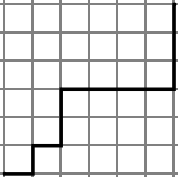
\includegraphics[width=\linewidth]{images/fig-lattice-path-6.png}
\end{image}%
\tcblower
\end{figureptx}%
\end{divisionexerciseeg}%
\begin{divisionexerciseeg}{7}{}{}{g:exercise:idm218170621952}%
Consider the set of lattice paths from \((0,0)\) to \((8,8)\).  You should know one quick formula for the cardinality of that set.  However, counting a different way can lead to an interesting  identity involving binomial coefficients.  Notice that any path goes through exactly one of the points \((0,8), (1,7), (2,6), \dots , (8,0)\).  Count the number of lattice paths that go through each of those 9 points - leave the expression in terms of binomial coefficients.  Even more interesting is what you get if  generalize to a destination of \((n,n)\), \(n \geq 1\).%
\end{divisionexerciseeg}%
\end{exercisegroup}
\par\medskip\noindent
\end{exercises-subsection-numberless}
\end{sectionptx}
%
%
\typeout{************************************************}
\typeout{Section 5.3 Some Lattices}
\typeout{************************************************}
%
\begin{sectionptx}{Some Lattices}{}{Some Lattices}{}{}{x:section:handouts-5}
Here are a couple of lattices for you to doodle with.%
\begin{figureptx}{}{g:figure:idm218170615744}{}%
\begin{image}{0.175}{0.65}{0.175}%
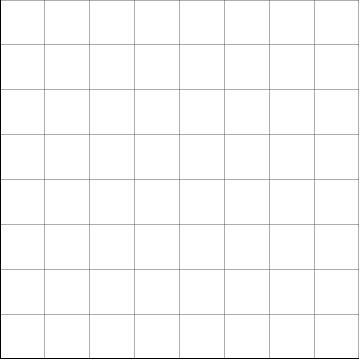
\includegraphics[width=\linewidth]{images/graphpaper8.png}
\end{image}%
\tcblower
\end{figureptx}%
\begin{figureptx}{}{g:figure:idm218170614576}{}%
\begin{image}{0.175}{0.65}{0.175}%
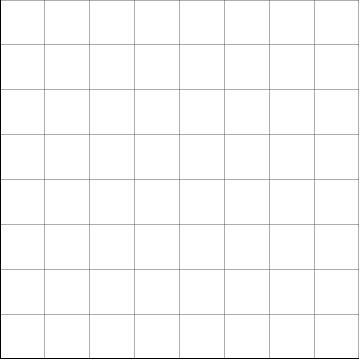
\includegraphics[width=\linewidth]{images/graphpaper8.png}
\end{image}%
\tcblower
\end{figureptx}%
\end{sectionptx}
\end{chapterptx}
 %
%
\typeout{************************************************}
\typeout{Chapter 6 Logic: Propositions and Truth Tables}
\typeout{************************************************}
%
\begin{chapterptx}{Logic: Propositions and Truth Tables}{}{Logic: Propositions and Truth Tables}{}{}{x:chapter:chapter_6}
\index{Propositions and Truth Tables}%
%
%
\typeout{************************************************}
\typeout{Section 6.1 Reading Assignment}
\typeout{************************************************}
%
\begin{sectionptx}{Reading Assignment}{}{Reading Assignment}{}{}{x:section:reading-6}
Read sections 3.1 and 3.2 of Applied Discrete Structures.  In Logic, we focus on the truth values of propositions, which are declarative sentences that are either true or false.  Later we will consider propositions that involve variables that determine the truth of a proposition. But for now, we focus on how propositions can be combined to create new propositions, much as we combine numbers to get other numbers.%
\begin{question}{Response Question.}{g:question:idm218170612064}%
Suppose you were given a proposition generated by 100 propositional variables and you are asked whether there is at least one assignment of truth values that you could assign to these variables to make the proposition true. Why is constructing a truth table not practical.  If you decided to examine all possible assignments of truth values and your computer could check one million cases per second, approximately how long would it take to check all cases?%
\end{question}
Also, turn in solutions to these exercises:%
%
%
\typeout{************************************************}
\typeout{Exercises 6.1 Exercises}
\typeout{************************************************}
%
\begin{exercises-subsection-numberless}{Exercises}{}{Exercises}{}{}{g:exercises:idm218170609312}
\par\medskip\noindent%
%
\begin{exercisegroup}
\begin{divisionexerciseeg}{1}{}{}{g:exercise:idm218170609056}%
For each of the following propositions, identify simple propositions, express the compound proposition in symbolic form, and determine whether it is true or false:%
\par
%
\begin{enumerate}[label=(\alph*)]
\item{}The world is flat or zero is an even integer.%
\item{}If 432,802 is a multiple of 4, then 432,802 is even.%
\item{}5 is a prime number and 6 is not divisible by 4.%
\item{}\(3 \in \mathbb{Z}\) and \(3 \in  \mathbb{Q}\).%
\item{}\(2/3 \in  \mathbb{Z}\) and \(2/3 \in  \mathbb{Q}\).%
\item{}The sum of two even integers is even and the sum of two odd integers is odd.%
\end{enumerate}
%
\end{divisionexerciseeg}%
\begin{divisionexerciseeg}{2}{}{}{g:exercise:idm218170603376}%
Construct the truth tables of:%
\begin{multicols}{2}
\begin{enumerate}[label=(\alph*)]
\item{}\(\displaystyle \neg (p\land  q )\)%
\item{}\(\displaystyle (p \land q)\land r\)%
\end{enumerate}
\end{multicols}
%
\end{divisionexerciseeg}%
\end{exercisegroup}
\par\medskip\noindent
\end{exercises-subsection-numberless}
\end{sectionptx}
%
%
\typeout{************************************************}
\typeout{Section 6.2 In-Class Exercises}
\typeout{************************************************}
%
\begin{sectionptx}{In-Class Exercises}{}{In-Class Exercises}{}{}{x:section:questions-6}
%
%
%
\typeout{************************************************}
\typeout{Exercises 6.2 Exercises}
\typeout{************************************************}
%
\begin{exercises-subsection-numberless}{Exercises}{}{Exercises}{}{}{g:exercises:idm218170600032}
\par\medskip\noindent%
%
\begin{exercisegroup}
\begin{divisionexerciseeg}{1}{}{}{g:exercise:idm218170599776}%
Reword the following statements into ``If...then'' statements.%
\begin{enumerate}[label=(\alph*)]
\item{}No resident of Chelmsford likes hot peppers.%
\item{}For 3+7=10, it is necessary that cows fly.%
\item{}For 3+7=10, it is sufficient that cows fly.%
\item{}Lowell is the oldest city in Massachusetts unless mermaids exist.%
\item{}I carry an umbrella when it rains.%
\end{enumerate}
%
\end{divisionexerciseeg}%
\begin{divisionexerciseeg}{2}{}{}{g:exercise:idm218170595936}%
Construct the truth table for \((p \lor q) \land (p\lor \neg q)\).   Notice anything about the result?%
\end{divisionexerciseeg}%
\begin{divisionexerciseeg}{3}{}{}{g:exercise:idm218170594944}%
Consider the statement “If Boris visits Hampton Beach, then he eats fried clams.”%
\begin{enumerate}[label=(\alph*)]
\item{}Write the converse of the statement.%
\item{}Write the contrapositive of the statement.%
\item{}Is it possible for the contrapositive to be false? If it was, what would that tell you?%
\item{}Suppose the original statement is true, and that Boris eats fried clams. Can you conclude anything (about his travels)?%
\item{}Suppose the original statement is true, and that Boris does not eat fried clams. Can you conclude anything (about his travels)?%
\end{enumerate}
%
\end{divisionexerciseeg}%
\begin{divisionexerciseeg}{4}{}{}{g:exercise:idm218170590624}%
Consider the statement, ``If a number is triangular or square, then it is not prime''%
\begin{enumerate}[label=(\alph*)]
\item{}Make a truth table for the statement \((T \vee S) \rightarrow \neg P\).%
\item{}If you believed the statement was false, what properties would a counterexample need to possess? Explain by referencing your truth table.%
\item{}If the statement were true, what could you conclude about the number 5657, which is definitely prime? Again, explain using the truth table.%
\end{enumerate}
%
\end{divisionexerciseeg}%
\end{exercisegroup}
\par\medskip\noindent
\end{exercises-subsection-numberless}
\end{sectionptx}
\end{chapterptx}
 %
%
\typeout{************************************************}
\typeout{Chapter 7 Equivalence, Implication, and Laws of Logic}
\typeout{************************************************}
%
\begin{chapterptx}{Equivalence, Implication, and Laws of Logic}{}{Equivalence, Implication, and Laws of Logic}{}{}{x:chapter:chapter_7}
\index{Equivalence}%
\index{Implication}%
\index{Laws of Logic}%
%
%
\typeout{************************************************}
\typeout{Section 7.1 Reading Assignment}
\typeout{************************************************}
%
\begin{sectionptx}{Reading Assignment}{}{Reading Assignment}{}{}{x:section:reading-7}
Read sections 3.3 and 3.4 of Applied Discrete Structures. Two propositions may be totally unrelated.  For example, ``It snowed today.'' and ``I played chess today.'' are likely to be unrelated.  Yet ``It snowed today.'' and ``I played golf today.'' are two propositions that are related in that it is unlikely that both are true.  In these two sections we introduce the ideas of equivalence and implication, which give us a precise way to talk about how propositions are related.%
\begin{question}{Response Question.}{g:question:idm218170582128}%
Explain why every proposition implies a tautology.%
\end{question}
Also, turn in solutions to these exercises:%
%
%
\typeout{************************************************}
\typeout{Exercises 7.1 Exercises}
\typeout{************************************************}
%
\begin{exercises-subsection-numberless}{Exercises}{}{Exercises}{}{}{g:exercises:idm218170580944}
\par\medskip\noindent%
%
\begin{exercisegroup}
\begin{divisionexerciseeg}{1}{}{}{g:exercise:idm218170580688}%
%
\begin{enumerate}[label=(\alph*)]
\item{}Construct the truth table for \(x= (p \land  \neg q) \lor  (r \land  p)\).%
\item{}Find an example other than \(x\) itself of a proposition generated by \(p\), \(q\), and \(r\) that is equivalent to \(x\).%
\item{}Find an example of a proposition that is not equivalent to \(x\) or a contradiction  that implies \(x\).%
\item{}Find an example of a proposition that is not equivalent to \(x\) or a tautology that is implied by \(x\).%
\end{enumerate}
%
\end{divisionexerciseeg}%
\begin{divisionexerciseeg}{2}{}{}{g:exercise:idm218170573280}%
Show that the common fallacy \((p\to  q) \land  \neg p \Rightarrow  \neg q\) is not a law of logic.%
\end{divisionexerciseeg}%
\end{exercisegroup}
\par\medskip\noindent
\end{exercises-subsection-numberless}
\end{sectionptx}
%
%
\typeout{************************************************}
\typeout{Section 7.2 In-Class Exercises}
\typeout{************************************************}
%
\begin{sectionptx}{In-Class Exercises}{}{In-Class Exercises}{}{}{x:section:questions-7}
%
%
%
\typeout{************************************************}
\typeout{Exercises 7.2 Exercises}
\typeout{************************************************}
%
\begin{exercises-subsection-numberless}{Exercises}{}{Exercises}{}{}{g:exercises:idm218170571744}
\par\medskip\noindent%
%
\begin{exercisegroup}
\begin{divisionexerciseeg}{1}{}{}{g:exercise:idm218170571488}%
Find a proposition that is equivalent to \(p \lor  q\) and uses only conjunction and negation.%
\end{divisionexerciseeg}%
\begin{divisionexerciseeg}{2}{}{}{g:exercise:idm218170570496}%
Frankie Fib was telling you what he consumed yesterday afternoon. He tells you, ``I had either popcorn or raisins. Also, if I had cucumber sandwiches, then I had soda. But I didn't drink soda or tea.'' Of course you know that Frankie is the worlds worst liar, and everything he says is false. What did Frankie have to eat and drink?%
\end{divisionexerciseeg}%
\begin{divisionexerciseeg}{3}{}{}{g:exercise:idm218170568880}%
Construct the truth table for \((p \rightarrow q) \land (q \rightarrow r) \land (r \rightarrow p)\).   Notice anything about the result?%
\end{divisionexerciseeg}%
\begin{divisionexerciseeg}{4}{}{}{g:exercise:idm218170569616}%
The significance of the Sheffer Stroke is that it is a ``universal'' operation in that all other logical operations can be built from it.%
\begin{enumerate}[label=(\alph*)]
\item{}Prove that \(p | q\) is equivalent to \(\neg (p \land  q)\).%
\item{}Prove that \(\neg p \Leftrightarrow  p | p\).%
\item{}Build \(\land\) using only the Sheffer Stroke.%
\item{}Build \(\lor\) using only the Sheffer Stroke.%
\end{enumerate}
%
\end{divisionexerciseeg}%
\end{exercisegroup}
\par\medskip\noindent
\end{exercises-subsection-numberless}
\end{sectionptx}
%
%
\typeout{************************************************}
\typeout{Section 7.3 The Sheffer Stroke}
\typeout{************************************************}
%
\begin{sectionptx}{The Sheffer Stroke}{}{The Sheffer Stroke}{}{}{x:section:handouts-7}
\index{Equivalence}%
Another logical operation is the Sheffer Stroke, which is the subject of one of the exercises.%
\begin{tableptx}{\textbf{Truth Table for the Sheffer Stroke}}{x:table:tt-scheffer}{}%
\centering%
{\tabularfont%
\begin{tabular}{ccc}
\(p\)&\(q\)&\(p \mid q\)\tabularnewline[0pt]
0&0&1\tabularnewline[0pt]
0&1&1\tabularnewline[0pt]
1&0&1\tabularnewline[0pt]
1&1&0
\end{tabular}
}%
\end{tableptx}%
\end{sectionptx}
\end{chapterptx}
 %
%
\typeout{************************************************}
\typeout{Chapter 8 Structured Proofs}
\typeout{************************************************}
%
\begin{chapterptx}{Structured Proofs}{}{Structured Proofs}{}{}{x:chapter:chapter_8}
\index{Proofs}%
%
%
\typeout{************************************************}
\typeout{Section 8.1 Reading Assignment}
\typeout{************************************************}
%
\begin{sectionptx}{Reading Assignment}{}{Reading Assignment}{}{}{x:section:reading-8}
Read section 3.5 of Applied Discrete Structures.  We can say that there are various relationships between propositions, but it might not be obvious that what we say is really true.  A proof is meant to be a means by which one can be convinced that such a relationship is true. Proofs are central to mathematics and appear in all remaining chapters in this book.  In Section 3.5 we start by identifying two basic types of proof: direct and indirect.%
\begin{question}{Response Question.}{g:question:idm218170552208}%
A proposition, \(P\), generated by a set of propositional variables is said to be satisfiable if there is at least one way to assign truth values to all of the variables so that \(P\) Is true. Explain why \(P\) is satisfiable as long as \(\neg P\)  is not a tautology.%
\end{question}
Also, turn in solutions to these exercises.%
%
%
\typeout{************************************************}
\typeout{Exercises 8.1 Exercises}
\typeout{************************************************}
%
\begin{exercises-subsection-numberless}{Exercises}{}{Exercises}{}{}{g:exercises:idm218170549040}
\par\medskip\noindent%
%
\begin{exercisegroup}
\begin{divisionexerciseeg}{1}{}{}{g:exercise:idm218170548784}%
Put the following into symbolic form and check its validity: If I am a good person, nothing bad will happen to me. Nothing happened to me. Therefore, I am a good person.%
\end{divisionexerciseeg}%
\begin{divisionexerciseeg}{2}{}{}{g:exercise:idm218170547936}%
Give  a direct or indirect proof of:%
\begin{equation*}
p\rightarrow  q, \neg r\rightarrow  \neg q, \neg r \Rightarrow  \neg p
\end{equation*}
%
\end{divisionexerciseeg}%
\end{exercisegroup}
\par\medskip\noindent
\end{exercises-subsection-numberless}
\end{sectionptx}
%
%
\typeout{************************************************}
\typeout{Section 8.2 In-Class Exercises}
\typeout{************************************************}
%
\begin{sectionptx}{In-Class Exercises}{}{In-Class Exercises}{}{}{x:section:questions-8}
%
%
%
\typeout{************************************************}
\typeout{Exercises 8.2 Exercises}
\typeout{************************************************}
%
\begin{exercises-subsection-numberless}{Exercises}{}{Exercises}{}{}{g:exercises:idm218170546368}
\par\medskip\noindent%
%
\begin{exercisegroup}
\begin{divisionexerciseeg}{1}{}{}{g:exercise:idm218170546032}%
Prove either directly or indirectly:%
\begin{equation*}
a \lor  b, c \land  d, a \rightarrow  \neg c \Rightarrow  b
\end{equation*}
%
\end{divisionexerciseeg}%
\begin{divisionexerciseeg}{2}{}{}{g:exercise:idm218170544736}%
In these two Lewis Carroll puzzles, you are given premises and are expected to form your own conclusion.  In each of them, convert the premises to symbolic form, draw a conclusion, and then translate back to English.%
\begin{enumerate}[label=(\alph*)]
\item{}%
\begin{itemize}[label=\textbullet]
\item{}No bald creature needs a hairbrush.%
\item{}No lizards have hair.%
\end{itemize}
%
\item{}%
\begin{itemize}[label=\textbullet]
\item{}Promise breakers are untrustworthy.%
\item{}Wine drinkers are very communicative.%
\item{}A man who keeps his promises is honest.%
\item{}No teetotalers are pawnbrokers.%
\item{}One can always trust a very communicative person.%
\end{itemize}
%
\end{enumerate}
%
\end{divisionexerciseeg}%
\begin{divisionexerciseeg}{3}{}{}{g:exercise:idm218170545152}%
There are \(n+1\), \(n\ge 1\) people who want to go to a concert.  All have different ages. You have three tickets: a back-stage pass and two regular (but distinguishable) tickets. Here are the rules for passing out the tickets:%
\begin{itemize}[label=\textbullet]
\item{}The backstage pass must go to the oldest person who gets a ticket.%
\item{}The person who gets the backstage pass can' t get either of the other two tickets, but the two regular tickets can both go to the same person.%
\end{itemize}
How many ways can you give away the tickets? There are two ways to count. Find both and equate them.%
\end{divisionexerciseeg}%
\end{exercisegroup}
\par\medskip\noindent
\end{exercises-subsection-numberless}
\end{sectionptx}
%
%
\typeout{************************************************}
\typeout{Section 8.3 Basic Logical Inferences}
\typeout{************************************************}
%
\begin{sectionptx}{Basic Logical Inferences}{}{Basic Logical Inferences}{}{}{x:section:handouts-8}
From section 3.4 of Applied Discrete Structures:%
\begin{tableptx}{\textbf{Basic Logical Laws - Common Implications and Equivalences}}{x:table:table-implications}{}%
\index{Modus Ponens!see Detachment}%
\index{Modus Tollens!see Indirect Reasoning}%
\index{Detachment}%
\index{Indirect Reasoning}%
\centering%
{\tabularfont%
\begin{tabular}{cc}
Detachment (AKA Modus Ponens)&\((p \rightarrow  q) \land  p\Rightarrow  q\)\tabularnewline\hrulemedium
Indirect Reasoning (AKA Modus Tollens)&\((p \to  q) \land  \neg q \Rightarrow  \neg p\)\tabularnewline\hrulemedium
Disjunctive Addition&\(p\Rightarrow (p\lor q)\)\tabularnewline\hrulemedium
Conjunctive Simplification&\((p \land  q) \Rightarrow  p\) and \((p \land  q) \Rightarrow  q\)\tabularnewline\hrulemedium
Disjunctive Simplification&\((p \lor  q) \land  \neg p \Rightarrow  q\) and \((p \lor q) \land \neg q\Rightarrow p\)\tabularnewline\hrulemedium
Chain Rule&\((p \to  q) \land  ( q \rightarrow  r) \Rightarrow  (p\to  r)\)\tabularnewline\hrulemedium
Conditional Equivalence&\(p \rightarrow  q \Leftrightarrow  \neg p \lor  q\)\tabularnewline\hrulemedium
Biconditional Equivalences&\((p \leftrightarrow  q) \Leftrightarrow  (p\rightarrow q) \land  (q \rightarrow  p)\Leftrightarrow (p \land  q) \lor  (\neg p \land  \neg q)\)\tabularnewline\hrulemedium
Contrapositive&\((p\to q) \Leftrightarrow (\neg q \to \neg p)\)
\end{tabular}
}%
\end{tableptx}%
\end{sectionptx}
\end{chapterptx}
 %
%
\typeout{************************************************}
\typeout{Chapter 9 Mathematical Induction}
\typeout{************************************************}
%
\begin{chapterptx}{Mathematical Induction}{}{Mathematical Induction}{}{}{x:chapter:chapter_9}
\index{}%
%
%
\typeout{************************************************}
\typeout{Section 9.1 Reading Assignment}
\typeout{************************************************}
%
\begin{sectionptx}{Reading Assignment}{}{Reading Assignment}{}{}{x:section:reading-9}
Read Sections 3.6 and 3.7 of \emph{Applied Discrete Structures}. It is only necessary to read 3.6 through Example 3.6.7.   The main idea in this reading is Mathematical Induction, which is a proof technique for propositions that have an integer variable.  This type of proof is used throughout mathematics and is particularly prevalent in discrete settings.%
\begin{question}{Response Question.}{g:question:idm218170518256}%
You don’t need induction to prove that the sum of the first \(n\) Positive integers equals \(\frac{n(n+1)}{2}\). Google “Gauss sum of consecutive integers” and read about how you can do it even more simply. Explain what you read.%
\end{question}
Also, turn in solutions to these exercises.%
%
%
\typeout{************************************************}
\typeout{Exercises 9.1 Exercises}
\typeout{************************************************}
%
\begin{exercises-subsection-numberless}{Exercises}{}{Exercises}{}{}{g:exercises:idm218170515936}
\par\medskip\noindent%
%
\begin{exercisegroup}
\begin{divisionexerciseeg}{1}{}{}{g:exercise:idm218170515680}%
Simplify the expressions%
\begin{enumerate}[label=(\alph*)]
\item{}\(\displaystyle (\sum_{k=1}^{n+1}k^2) -(\sum_{k=1}^n k^2)\)%
\item{}\(\displaystyle \sum_{k=1}^n (\frac{1}{k}-\frac{1}{k+1})\)%
\item{}\(\displaystyle \frac{(n+2)!}{n!}\)%
\end{enumerate}
%
\end{divisionexerciseeg}%
\begin{divisionexerciseeg}{2}{}{}{g:exercise:idm218170513184}%
Prove that for \(n \ge 0\), \(\sum_{k=0}^n {2^k} = 2^{n+1}-1\).%
\par\smallskip%
\noindent\textbf{\blocktitlefont Solution}.\hypertarget{g:solution:idm218170510912}{}\quad{}Let \(p(n)\) be the proposition \(\sum_{k=0}^{n} 2^k = 2^{n+1}-1\), \(n\geq 0\).  The basis of an induction proof that this proposition is a tautology is to observe that if \(n=0\) we have \(2^0 = 2^{0+1}-1\), which is true.%
\par
Now the induction step of the proof calls for assuming that for some \(n \geq 0\), \(p(n)\) is true (this is the ``induction hypothesis'').   We then proof that \(p(n+1)\) follows from the induction hypothesis.%
\begin{equation*}
\begin{split}
\sum_{k=0}^{n+1} {2^k} &= \sum_{k=0}^n {2^k} +2^{n+1}\\
&= (2^{n+1}-1) + 2^{n+1} \quad\quad\textrm{by the induction hypothesis}\\
&= 2^{n+2}-1\\ 
&= 2^{(n+1)+1}-1
\end{split}
\end{equation*}
and we are done!%
\end{divisionexerciseeg}%
\end{exercisegroup}
\par\medskip\noindent
\end{exercises-subsection-numberless}
\end{sectionptx}
%
%
\typeout{************************************************}
\typeout{Section 9.2 In-Class Exercises}
\typeout{************************************************}
%
\begin{sectionptx}{In-Class Exercises}{}{In-Class Exercises}{}{}{x:section:questions-9}
%
%
%
\typeout{************************************************}
\typeout{Exercises 9.2 Exercises}
\typeout{************************************************}
%
\begin{exercises-subsection-numberless}{Exercises}{}{Exercises}{}{}{g:exercises:idm218170505056}
\par\medskip\noindent%
%
\begin{exercisegroup}
\begin{divisionexerciseeg}{1}{}{}{g:exercise:idm218170504720}%
Prove that for \(n\geq 1\),%
\begin{equation*}
\frac{1}{1\cdot 2 }+ \frac{1}{2\cdot 3}+ \cdots  + \frac{1}{n(n+1)}= \frac{n}{n+1}.
\end{equation*}
%
\end{divisionexerciseeg}%
\begin{divisionexerciseeg}{2}{}{}{x:exercise:stamp-problem}%
Prove that it is possible to make up any postage of 28 cents or more using only five-cent and eight-cent stamps.%
\end{divisionexerciseeg}%
\begin{divisionexerciseeg}{3}{}{}{g:exercise:idm218170502288}%
Suppose that a particular real number \(x\) has the property that \(x + \frac{1}{x}\) is an integer.  Prove that \(x^n + \frac{1}{x^n}\) is an integer for all natural numbers \(n\).%
\end{divisionexerciseeg}%
\end{exercisegroup}
\par\medskip\noindent
\end{exercises-subsection-numberless}
\end{sectionptx}
\end{chapterptx}
 %
%
\typeout{************************************************}
\typeout{Chapter 10 Quantifiers and Proof Review}
\typeout{************************************************}
%
\begin{chapterptx}{Quantifiers and Proof Review}{}{Quantifiers and Proof Review}{}{}{x:chapter:chapter_10}
\index{}%
%
%
\typeout{************************************************}
\typeout{Section 10.1 Reading Assignment}
\typeout{************************************************}
%
\begin{sectionptx}{Reading Assignment}{}{Reading Assignment}{}{}{x:section:reading-10}
Read Sections 3.8 and 3.9 of \emph{Applied Discrete Structures}.  Quantifiers are used to say something about the truth sets of propositions.  You will read about two basic ones (Universal and Existential).  Individually, they are fairly simple.  Where things can be tricky is when when you have more than one variable and you mix the two types of quantifiers, or you negate a quantified expression.  Pay close attention to these situations.%
\begin{question}{Response Question.}{g:question:idm218170497200}%
In reviewing a certain local coffee roaster, a writer stated  "...but all of its coffee is not fair trade." The writer was rebutting a claim by the roaster that "All of our coffee is fair trade."  Explain why the reviewer's statement was incorrect.%
\end{question}
Also, turn in solutions to these exercises:%
%
%
\typeout{************************************************}
\typeout{Exercises 10.1 Exercises}
\typeout{************************************************}
%
\begin{exercises-subsection-numberless}{Exercises}{}{Exercises}{}{}{g:exercises:idm218170495760}
\par\medskip\noindent%
%
\begin{exercisegroup}
\begin{divisionexerciseeg}{1}{}{}{g:exercise:idm218170495504}%
Let \(M(x)\) be ``\(x\) is a mammal,'' let \(A(x)\) be ``\(x\) is an animal,'' and let \(W(x)\) be ``\(x\) is warm-blooded.''%
\par
%
\begin{enumerate}[label=(\alph*)]
\item{}Translate into a formula: Every mammal is warm-blooded.%
\item{}Translate into English: \((\exists x)(A(x) \land  (\neg M(x)))\).%
\end{enumerate}
%
\end{divisionexerciseeg}%
\begin{divisionexerciseeg}{2}{}{}{g:exercise:idm218170489296}%
Write out a complete proof that if \(n\) is an integer, \(n^2\) is even if and only if \(n\) is even.%
\end{divisionexerciseeg}%
\end{exercisegroup}
\par\medskip\noindent
\end{exercises-subsection-numberless}
\end{sectionptx}
%
%
\typeout{************************************************}
\typeout{Section 10.2 In-Class Exercises}
\typeout{************************************************}
%
\begin{sectionptx}{In-Class Exercises}{}{In-Class Exercises}{}{}{x:section:questions-10}
%
%
%
\typeout{************************************************}
\typeout{Exercises 10.2 Exercises}
\typeout{************************************************}
%
\begin{exercises-subsection-numberless}{Exercises}{}{Exercises}{}{}{g:exercises:idm218170486944}
\par\medskip\noindent%
%
\begin{exercisegroup}
\begin{divisionexerciseeg}{1}{}{}{g:exercise:idm218170486688}%
Translate the following statement over the positive integers into symbols. Use \(E(x)\) for ``\(x\) is even'' and \(O(x)\) for ``\(x\) is odd'' in the first three parts.%
\begin{enumerate}[label=(\alph*)]
\item{}No number is both even and odd.%
\item{}One more than any even number is an odd number.%
\item{}There is prime number that is even.%
\item{}Between any two numbers there is a third number.%
\item{}There is no number between a number and one more than that number.%
\end{enumerate}
%
\end{divisionexerciseeg}%
\begin{divisionexerciseeg}{2}{}{}{g:exercise:idm218170486304}%
Use quantifiers to state that for every positive integer, there is a larger positive integer.%
\end{divisionexerciseeg}%
\begin{divisionexerciseeg}{3}{}{}{g:exercise:idm218170480368}%
One of the following is true and the other is false.  Identify the true one says and explain why the other one is false.%
\begin{gather*}
(\exists  b)_{\mathbb{Z}} ((\forall a)_{\mathbb{Z}}(a + b = 0))\\
(\forall  a)_{\mathbb{Z}} ((\exists b)_{\mathbb{Z}}(a + b = 0))
\end{gather*}
%
\end{divisionexerciseeg}%
\begin{divisionexerciseeg}{4}{}{}{g:exercise:idm218170478704}%
Prove that the sum of of an odd integer and and even integer is odd.%
\end{divisionexerciseeg}%
\begin{divisionexerciseeg}{5}{}{}{g:exercise:idm218170478192}%
Prove that if you divide 4 into a perfect square, \(1, 4, 9, 16, \dots\), the remainder will be either 0 or 1.%
\end{divisionexerciseeg}%
\begin{divisionexerciseeg}{6}{}{}{g:exercise:idm218170477136}%
Prove that the cube root of \(2\) is an irrational number.%
\end{divisionexerciseeg}%
\end{exercisegroup}
\par\medskip\noindent
\end{exercises-subsection-numberless}
\end{sectionptx}
\end{chapterptx}
 %
%
\typeout{************************************************}
\typeout{Chapter 11 Set Theory Logic}
\typeout{************************************************}
%
\begin{chapterptx}{Set Theory Logic}{}{Set Theory Logic}{}{}{x:chapter:chapter_11}
%
%
\typeout{************************************************}
\typeout{Section 11.1 Reading Assignment}
\typeout{************************************************}
%
\begin{sectionptx}{Reading Assignment}{}{Reading Assignment}{}{}{x:section:reading-11}
Read Sections 4.1  and 4.2 of \emph{Applied Discrete Structures}.  In these sections, we revisit some of the set theory from Chapter 1, applying some of the logic in Chapter 3. Be aware of the types of objects that are in the sets involved in a proof.  One example is that when you are proving something about Cartesian products, the objects usually need to be identified as ordered pairs, not simply as single variables.%
\begin{question}{Response Question.}{g:question:idm218170473808}%
Compare the Laws of Set Theory in Section 4.2 of Applied Discrete Structures with the Basic Laws of Logic in Section 3.5 of Applied Discrete Structures.  Focus on any two different laws of set theory that you choose and discuss how they are similar to two logic laws.%
\end{question}
Also, turn in solutions to these exercises:%
%
%
\typeout{************************************************}
\typeout{Exercises 11.1 Exercises}
\typeout{************************************************}
%
\begin{exercises-subsection-numberless}{Exercises}{}{Exercises}{}{}{g:exercises:idm218170472512}
\par\medskip\noindent%
%
\begin{exercisegroup}
\begin{divisionexerciseeg}{1}{}{}{g:exercise:idm218170472256}%
Write the converse of the following true statements and prove or disprove them.%
\begin{enumerate}[label=(\alph*)]
\item{}Let \(A\), \(B\), and \(C\) be sets. If \(A\subseteq B\) and \(B\subseteq C\), then \(A\subseteq C\).%
\item{}Let \(A,B, \textrm{ and } C\) be sets. If (\(A\subseteq B\) and \(A\subseteq C\)) then \(A\subseteq B\cap C\).%
\item{}Let \(A,B, \textrm{ and } C\) be sets with \(C\neq \emptyset\). If \(A\subseteq B\) then \(A\times C \subseteq B\times C\).%
\end{enumerate}
%
\end{divisionexerciseeg}%
\begin{divisionexerciseeg}{2}{}{}{g:exercise:idm218170463504}%
%
\begin{enumerate}[label=(\alph*)]
\item{}Prove the Identity Law for sets  with a membership table.%
\item{}Prove the Involution Law  for sets using basic definitions.%
\end{enumerate}
%
\end{divisionexerciseeg}%
\end{exercisegroup}
\par\medskip\noindent
\end{exercises-subsection-numberless}
\end{sectionptx}
%
%
\typeout{************************************************}
\typeout{Section 11.2 In-Class Exercises}
\typeout{************************************************}
%
\begin{sectionptx}{In-Class Exercises}{}{In-Class Exercises}{}{}{x:section:questions-11}
%
%
%
\typeout{************************************************}
\typeout{Exercises 11.2 Exercises}
\typeout{************************************************}
%
\begin{exercises-subsection-numberless}{Exercises}{}{Exercises}{}{}{g:exercises:idm218170461552}
\par\medskip\noindent%
%
\begin{exercisegroup}
\begin{divisionexerciseeg}{1}{}{}{g:exercise:idm218170461296}%
What can one say about the sets \(A\) and \(B\) if we know the following?  Back up your answers with proofs.%
\begin{enumerate}[label=(\alph*)]
\item{}\(\displaystyle A \cup B = A\)%
\item{}\(\displaystyle A\cap B = A\)%
\item{}\(\displaystyle A–B = A\)%
\item{}\(\displaystyle A\cap B = B\cap A\)%
\item{}\(\displaystyle A–B = B–A\)%
\end{enumerate}
%
\end{divisionexerciseeg}%
\begin{divisionexerciseeg}{2}{}{}{g:exercise:idm218170456352}%
%
\begin{enumerate}[label=(\alph*)]
\item{}Given the following sets of integers, \(A, B, C\), find the set of elements that belong to exactly one of the three sets.%
\begin{gather*}
A=\{2,6,10,14,18\}\\
B=\{2,3,5,7,11,13,17,19\}\\
C=\{3,6,9,12,15,18\}
\end{gather*}
%
\item{}Prove that for any three sets, \(A, B, C\),%
\begin{equation*}
(A \cup B \cup C)\cap ((A^c \cap B^c)\cup (A^c \cap C^c)\cup (B^c \cap C^c))
\end{equation*}
is the set of all elements that belong to exactly one of the three sets.  Verify this fact first with the example in the previous part, where you assume that the universe is \(\{1,2,3,\dots,18,19\}\).%
\item{}Find a similar expression for the set of elements that belong to exactly one of any four sets \(A, B, C, D.\)%
\end{enumerate}
%
\end{divisionexerciseeg}%
\begin{divisionexerciseeg}{3}{}{}{g:exercise:idm218170450688}%
Recall that the power set of any set \(A\) is the set of all subsets of \(A\) and is denoted \(\mathcal{P}(A)\).  Which of the following are true?%
\begin{gather*}
\mathcal{P}(A \cap B) = \mathcal{P}(A) \cap \mathcal{P}(B)\\
\mathcal{P}(A \cup B) = \mathcal{P}(A) \cup \mathcal{P}(B)
\end{gather*}
If either is not true, can you replace the equals sign with \(\subseteq\) or \(\supseteq\) to get a true statement?%
\end{divisionexerciseeg}%
\end{exercisegroup}
\par\medskip\noindent
\end{exercises-subsection-numberless}
\end{sectionptx}
%
%
\typeout{************************************************}
\typeout{Section 11.3 The Basic Laws of Set Theory}
\typeout{************************************************}
%
\begin{sectionptx}{The Basic Laws of Set Theory}{}{The Basic Laws of Set Theory}{}{}{g:section:idm218170450304}
\begin{tableptx}{\textbf{Basic Laws of Set Theory}}{x:table:table-set-laws}{}%
\centering%
{\tabularfont%
\begin{tabular}{ccc}
&&\tabularnewline[0pt]
&Commutative Laws&\tabularnewline[0pt]
(1) \(A \cup B = B \cup  A\)&&(\(1^{\prime}\)) \(A \cap B = B\cap A\)\tabularnewline\hrulethin
&Associative Laws&\tabularnewline[0pt]
(2) \(A \cup  (B \cup  C)= (A\cup B)\cup C\)&&(\(2^{\prime}\)) \(A \cap  (B \cap  C) = (A \cap  B) \cap  C \)\tabularnewline\hrulethin
&Distributive Laws&\tabularnewline[0pt]
(3) \(A\cap (B \cup  C)=(A\cap B )\cup (A\cap  C)\)&&(\(3^{\prime}\)) \(A \cup (B \cap C) = (A \cup B ) \cap (A\cup C)\)\tabularnewline\hrulethin
&Identity Laws&\tabularnewline[0pt]
(4) \(A \cup  \emptyset  = \emptyset  \cup  A = A\)&&(\(4^{\prime}\)) \(A \cap  U = U \cap  A = A\)\tabularnewline\hrulethin
&Complement Laws&\tabularnewline[0pt]
(5) \(A\cup A^c= U\)&&(\(5^{\prime}\)) \(A\cap A^c= \emptyset\)\tabularnewline\hrulethin
&Idempotent Laws&\tabularnewline[0pt]
(6) \(A \cup  A = A\)&&(\(6^{\prime}\)) \(A\cap  A = A\)\tabularnewline\hrulethin
&Null Laws&\tabularnewline[0pt]
(7) \(A \cup  U = U\)&&(\(7^{\prime}\)) \(A \cap  \emptyset  =\emptyset\)\tabularnewline\hrulethin
&Absorption Laws&\tabularnewline[0pt]
(8) \(A \cup  (A\cap  B) = A\)&&(\(8^{\prime}\)) \(A\cap (A \cup  B) = A\)\tabularnewline\hrulethin
&DeMorgan's Laws&\tabularnewline[0pt]
(9) \((A \cup  B)^c= A^c\cap  B^c\)&&(\(9^{\prime}\)) \((A\cap  B)^c = A^c \cup  B^c\)\tabularnewline\hrulethin
&Involution Law&\tabularnewline[0pt]
&(10) \((A^c)^c= A\)&\tabularnewline\hrulethin
\end{tabular}
}%
\end{tableptx}%
\end{sectionptx}
\end{chapterptx}
 %
%
\typeout{************************************************}
\typeout{Chapter 12 Minsets and Duality}
\typeout{************************************************}
%
\begin{chapterptx}{Minsets and Duality}{}{Minsets and Duality}{}{}{x:chapter:chapter_12}
\index{}%
%
%
\typeout{************************************************}
\typeout{Section 12.1 Reading Assignment}
\typeout{************************************************}
%
\begin{sectionptx}{Reading Assignment}{}{Reading Assignment}{}{}{x:section:reading-12}
Read Sections 4.3 and 4.4 of \emph{Applied Discrete Structures}. Minsets help answer the question of what sets can be created if you start with a certain collection of sets and apply basic set operations to them.   Duality is an organizing principle that set theory shares with logic and a few other mathematical structures.%
\begin{question}{Response Question.}{g:question:idm218170415776}%
To what extend is there any duality in arithmetic of numbers with addition and multiplication?  How does it break down where it doesn't in set theory?%
\end{question}
Also, turn in solutions to these exercises:%
%
%
\typeout{************************************************}
\typeout{Exercises 12.1 Exercises}
\typeout{************************************************}
%
\begin{exercises-subsection-numberless}{Exercises}{}{Exercises}{}{}{g:exercises:idm218170414432}
\par\medskip\noindent%
%
\begin{exercisegroup}
\begin{divisionexerciseeg}{1}{}{}{g:exercise:idm218170414176}%
Consider the subsets \(A = \{1, 3, 5\}\), \(B = \{2,3,4\}\),  where \(U = \{1,2,3,4,5\}\).  List the nonempty minsets generated by \(A\textrm{ and }B\).%
\end{divisionexerciseeg}%
\begin{divisionexerciseeg}{2}{}{}{g:exercise:idm218170411632}%
What is the dual of \(A \cap (B\cap (A\cap B)^c)= \emptyset\)?%
\end{divisionexerciseeg}%
\end{exercisegroup}
\par\medskip\noindent
\end{exercises-subsection-numberless}
\end{sectionptx}
%
%
\typeout{************************************************}
\typeout{Section 12.2 In-Class Exercises}
\typeout{************************************************}
%
\begin{sectionptx}{In-Class Exercises}{}{In-Class Exercises}{}{}{x:section:questions-12}
%
%
%
\typeout{************************************************}
\typeout{Exercises 12.2 Exercises}
\typeout{************************************************}
%
\begin{exercises-subsection-numberless}{Exercises}{}{Exercises}{}{}{g:exercises:idm218170409920}
\par\medskip\noindent%
%
\begin{exercisegroup}
\begin{divisionexerciseeg}{1}{}{}{g:exercise:idm218170409664}%
A common way to denote a particular minset generated by a collection of subsets is as follows.  If there are \(k\) subsets, \(B_1, B_2, \dots ,B_k\), and \(b=b_1b_2\cdots b_k\) is any string of \(k\) bits, then%
\begin{equation*}
M_b =  M_{b_1b_2\cdots b_k} = D_1 \cap D_2 \cap \cdots \cap D_k,
\end{equation*}
where \(D_i\) is either \(B_i\) or \(B_i^c\).  If \(b_i = 1\) then \(D_i =B_i\) and if \(b_i=0\) then \(D_i=B_i^c\).  For example, if \(k=4\), \(M_{0110} = B_1^c \cap B_2 \cap B_3 \cap B_4^c\).%
\begin{enumerate}[label=(\alph*)]
\item{}Suppose \(U=\{1, 2, 3, 4, 5\}\), \(k=2\), \(B_1= \{1, 2\}\), and \(B_2 = \{2,3,4\}\).  List the nonempty minsets generated by \(B_1\) and \(B_2\) using ``\(M_b\)'' notation. Notice that they form a partition of \(U\).%
\item{}How does this notation make help us see how many distinct nonempty minsets there could be that are generated by \(k\) subsets of a universe.%
\end{enumerate}
%
\end{divisionexerciseeg}%
\begin{divisionexerciseeg}{2}{}{}{g:exercise:idm218170409280}%
%
\begin{enumerate}[label=(\alph*)]
\item{}Partition \(\{1, 2,  \dots, 8\}\) into the nonempty minsets generated by \(B_1= \{1, 2\}\), \(B_2 = \{1, 3, 5, 8\}\), and \(B_3 = \{2, 3, 4, 6\}\).%
\item{}How many different subsets of \(\{1, 2, \dots ,8\}\) can you create using \(B_1, B_2\), and \(B_3\) with the standard set operations?%
\item{}Do there exist subsets \(C_1, C_2, C_3\) with which you can generate every subset of \(\{1,2, . . . ,8\}\)?  If so, can you find such a collection of subsets?  If not, why?  You might find the Venn diagram below useful for thinking about this problem.%
\end{enumerate}
%
\begin{figureptx}{A three set Venn diagram}{x:figure:fig-venn3}{}%
\begin{image}{0.05}{0.9}{0.05}%
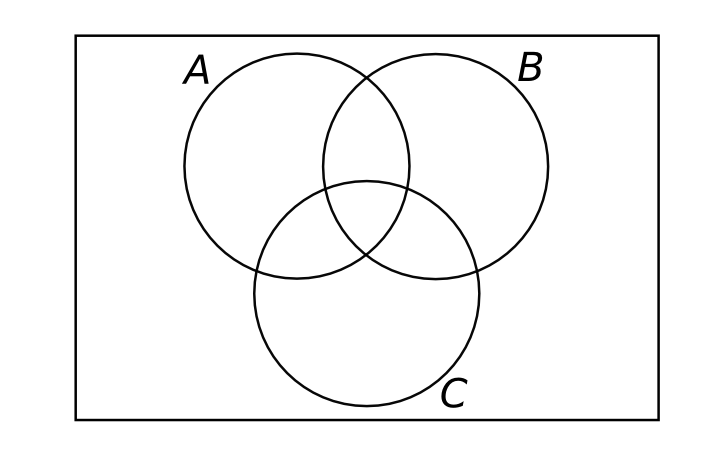
\includegraphics[width=\linewidth]{images/fig-venn3.png}
\end{image}%
\tcblower
\end{figureptx}%
\end{divisionexerciseeg}%
\begin{divisionexerciseeg}{3}{}{}{g:exercise:idm218170389504}%
What is the dual of a minset?  These sets are called ``maxsets''  Find the maxsets generated by the two sets in part (a) of the first problem.   Why do you suppose they are called maxsets?%
\end{divisionexerciseeg}%
\begin{divisionexerciseeg}{4}{}{}{g:exercise:idm218170388384}%
The descriptions of duality in Section 4.4 is not complete.  If you expand expressions involving subsets, such as the expression \(A \cap B \subseteq A\), which is a true statement in set theory.  What should be the dual?  How should we treat the subset symbol?%
\end{divisionexerciseeg}%
\end{exercisegroup}
\par\medskip\noindent
\end{exercises-subsection-numberless}
\end{sectionptx}
\end{chapterptx}
 %
%
\typeout{************************************************}
\typeout{Chapter 13 Matrix Operations}
\typeout{************************************************}
%
\begin{chapterptx}{Matrix Operations}{}{Matrix Operations}{}{}{x:chapter:chapter_13}
\index{Matrix Operations}%
%
%
\typeout{************************************************}
\typeout{Section 13.1 Reading Assignment}
\typeout{************************************************}
%
\begin{sectionptx}{Reading Assignment}{}{Reading Assignment}{}{}{x:section:reading-13}
Read Sections 5.1 and 5.2 of Applied Discrete Structures. Matrix algebra serves as a contrasting system to logic and set theory but is also needed in the study of relations in Chapter 6.  In these two sections, we review matrix operations and some special matrices.%
\begin{question}{Response Question.}{g:question:idm218170385104}%
Let \(A=\left(\begin{array}{cc} 2 & 0\\ 0 & -1 \end{array}\right)\). Select any 2 by 2 matrix with nonzero entries and call it \(B\). Compute the products \(AB \textrm{ and }BA\)  What effect does \(A\) have on \(B\) in each case?%
\end{question}
Also, turn in solutions to these exercises:%
%
%
\typeout{************************************************}
\typeout{Exercises 13.1 Exercises}
\typeout{************************************************}
%
\begin{exercises-subsection-numberless}{Exercises}{}{Exercises}{}{}{g:exercises:idm218170381808}
\par\medskip\noindent%
%
\begin{exercisegroup}
\begin{divisionexerciseeg}{1}{}{}{g:exercise:idm218170381552}%
Let \(A=\left(
\begin{array}{cc}
1 & -1 \\
2 & 3 \\
\end{array}
\right)\) and  \(B =\left(
\begin{array}{cc}
0 & 1 \\
3 & -5 \\
\end{array}
\right)\)%
\par
%
\begin{enumerate}[label=(\alph*)]
\item{}Compute \(A B\) and \(B A\).%
\item{}Compute \(A + B\) and \(B + A\).%
\end{enumerate}
%
\end{divisionexerciseeg}%
\begin{divisionexerciseeg}{2}{}{}{g:exercise:idm218170376640}%
For the given matrices \(A\) find \(A^{-1}\) if it exists and verify that \(A A^{-1}=A^{-1}A = I\). If \(A^{-1}\) does not exist explain why.%
\par
%
\begin{enumerate}[label=(\alph*)]
\item{}\(\displaystyle A =\left(
\begin{array}{cc}
2 & -1 \\
-1 & 2 \\
\end{array}
\right)\)%
\item{}\(\displaystyle A = \left(
\begin{array}{cc}
2 & 1 \\
4 & 2 \\
\end{array}
\right)\)%
\end{enumerate}
%
\end{divisionexerciseeg}%
\end{exercisegroup}
\par\medskip\noindent
\begin{conclusion}{}%
There is a short video on matrix multiplication at \url{https://youtu.be/zt-IU1lXFzs}%
\end{conclusion}%
\end{exercises-subsection-numberless}
\end{sectionptx}
%
%
\typeout{************************************************}
\typeout{Section 13.2 In-Class Exercises}
\typeout{************************************************}
%
\begin{sectionptx}{In-Class Exercises}{}{In-Class Exercises}{}{}{x:section:questions-13}
%
%
%
\typeout{************************************************}
\typeout{Exercises 13.2 Exercises}
\typeout{************************************************}
%
\begin{exercises-subsection-numberless}{Exercises}{}{Exercises}{}{}{g:exercises:idm218170370992}
\par\medskip\noindent%
%
\begin{exercisegroup}
\begin{divisionexerciseeg}{1}{}{}{g:exercise:idm218170370736}%
Let \(A=\left(\begin{array}{cc} 1 & a\\ 0 & 1 \end{array}\right)\) and \(B=\left(\begin{array}{cc} 1 & b\\ 0 & 1 \end{array}\right)\).  Compute the product \(A B\).  Based on this result, what is \(A^{-1}\).%
\end{divisionexerciseeg}%
\begin{divisionexerciseeg}{2}{}{}{g:exercise:idm218170368288}%
\index{Transpose of a matrix}%
If \(A\) is a an \(m \times n\) matrix, we define the transpose of A to be the \(n \times m\) matrix whose rows are the columns of \(A\).  For example, the transpose of%
\begin{equation*}
\left(
\begin{array}{ccc}
1 &2 &3 \\
4 &5 &6 \\
\end{array}
\right) \textrm{  is  }
\left(
\begin{array}{cc}
1 &4 \\
2 &5 \\
3 &6 \\
\end{array}
\right).
\end{equation*}
The notation \(A^t\) is used for the transpose of \(A\).%
\begin{enumerate}[label=(\alph*)]
\item{}If \(A\) is an \(m \times n\) matrix, are the products \(A A^t\) and \(A^t A \) defined?  What are the orders of the products that are defined?%
\item{}Given the following matrix, what useful information might you get from the products \(A A^t\) or \(A^t A\).?%
\begin{equation*}
A=\left(
\begin{array}{ccccc}
16 &11 &4 &3 &15 \\
16 &17 &13 &12 &6 \\
\end{array}
\right) 
\end{equation*}
%
\end{enumerate}
%
\end{divisionexerciseeg}%
\begin{divisionexerciseeg}{3}{}{}{g:exercise:idm218170367648}%
Prove by induction that for \(n \geq 1\), \(\left(
\begin{array}{cc}
a & 0 \\
0 & b \\
\end{array}
\right)^n= \left(
\begin{array}{cc}
a^n & 0 \\
0 & b^n \\
\end{array}
\right)\).%
\end{divisionexerciseeg}%
\begin{divisionexerciseeg}{4}{}{}{g:exercise:idm218170358000}%
In this exercise, we propose to show how matrix multiplication is a natural operation.  Suppose a bakery produces bread, cakes and pies every weekday, Monday through Friday. Based on past sales history, the bakery produces various numbers of each product each day, summarized in the \(5 \times 3\) matrix \(D\).  It should be noted that the order could be described as ``number of days by number of products.''   For example, on Wednesday (the third day) the number of cakes (second product in our list) that are produced  is  \(d_{3,2} = 4\).%
\begin{equation*}
D =\left(
\begin{array}{ccc}
25 & 5 & 5 \\
14 & 5 & 8 \\
20 & 4 & 15 \\
18 & 5 & 7 \\
35 & 10 & 9 \\
\end{array}
\right)
\end{equation*}
%
\par
The main ingredients of these products are flour, sugar and eggs. We assume that other ingredients are always in ample supply, but we need to be sure to have the three main ones available.   For each of the three products, The amount of each ingredient that is needed is summarized in the \(3 \times 3\), or ``number of products by number of ingredients'' matrix \(P\).  For example, to bake a cake (second product) we need \(P_{2,1}=1.5\) cups of flour (first ingredient).  Regarding units: flour and sugar are given in cups per unit of each product, while eggs are given in individual eggs per unit of each product.%
\begin{equation*}
P =\left(
\begin{array}{ccc}
2 & 0.5 & 0 \\
1.5 & 1 & 2 \\
1 & 1 & 1  \\
\end{array}
\right)
\end{equation*}
These amounts are ``made up'', so don't used them to do your own baking!%
\par
%
\begin{enumerate}[label=(\alph*)]
\item{}How many cups of flour will the bakery need every Monday?  Pay close attention to how you compute your answer and the units of each number.%
\item{}How many eggs will the bakery need every Wednesday?%
\item{}Compute the matrix product \(D P\).   What do you notice?%
\item{}Suppose the costs of ingredients are \(\$0.12\) for a cup of flour, \(\$0.15\) for a cup of sugar and \(\$0.19\) for one egg. How can this information be put into a matrix that can meaningfully be multiplied by one of the other matrices in this problem?%
\end{enumerate}
%
\end{divisionexerciseeg}%
\end{exercisegroup}
\par\medskip\noindent
\end{exercises-subsection-numberless}
\end{sectionptx}
\end{chapterptx}
 %
%
\typeout{************************************************}
\typeout{Chapter 14 Matrix Laws and Oddities}
\typeout{************************************************}
%
\begin{chapterptx}{Matrix Laws and Oddities}{}{Matrix Laws and Oddities}{}{}{x:chapter:chapter_14}
%
%
\typeout{************************************************}
\typeout{Section 14.1 Reading Assignment}
\typeout{************************************************}
%
\begin{sectionptx}{Reading Assignment}{}{Reading Assignment}{}{}{x:section:reading-14}
Read Sections 5.3 and 5.4 of \emph{Applied Discrete Structures}.  In these two sections we concentrate on the algebraic laws of set theory and some of the laws that are missing (because they are false!).%
\begin{question}{Response Question.}{g:question:idm218170344384}%
Compare Matrix Law (15), The Inverse of Product Rule, with the fact that although you put your socks on before your shoes, you take your shoes off before taking off your socks.%
\end{question}
Also, turn in solutions to these exercises:%
%
%
\typeout{************************************************}
\typeout{Exercises 14.1 Exercises}
\typeout{************************************************}
%
\begin{exercises-subsection-numberless}{Exercises}{}{Exercises}{}{}{g:exercises:idm218170343168}
\par\medskip\noindent%
%
\begin{exercisegroup}
\begin{divisionexerciseeg}{1}{}{}{g:exercise:idm218170342912}%
Let \(A=\left(\begin{array}{cccc} 0 &1&0&0\\
0 &0&1&0\\
0&0&0&1\\
1 &0&0&0 \end{array}\right)\). Compute \(A^2\), \(A^3\), \(A^4\), and \(A^{-1}\).%
\end{divisionexerciseeg}%
\begin{divisionexerciseeg}{2}{}{}{g:exercise:idm218170342528}%
Find at least three \(2\times2\) matrices, \(A\), such that \(A^2=A\).%
\end{divisionexerciseeg}%
\end{exercisegroup}
\par\medskip\noindent
\end{exercises-subsection-numberless}
\end{sectionptx}
%
%
\typeout{************************************************}
\typeout{Section 14.2 In-Class Exercises}
\typeout{************************************************}
%
\begin{sectionptx}{In-Class Exercises}{}{In-Class Exercises}{}{}{x:section:questions-14}
%
%
%
\typeout{************************************************}
\typeout{Exercises 14.2 Exercises}
\typeout{************************************************}
%
\begin{exercises-subsection-numberless}{Exercises}{}{Exercises}{}{}{g:exercises:idm218170337696}
\par\medskip\noindent%
%
\begin{exercisegroup}
\begin{divisionexerciseeg}{1}{}{}{g:exercise:idm218170337440}%
Let \(A\) and \(B\) be \(n\times n\) matrices of real numbers. Is \(A^2-B^2= (A-B)(A+B)\)?  Explain.%
\end{divisionexerciseeg}%
\begin{divisionexerciseeg}{2}{}{}{g:exercise:idm218170334960}%
Write each of the following systems in the form \(A X = B\), and then solve the systems using matrices.%
\par
%
\begin{multicols}{2}
\begin{enumerate}[label=(\alph*)]
\item{}\(\displaystyle \begin{array}{c}4x_1-6x_2=20\\
3x_1+5x_2= -6\\
\end{array}\)%
\item{}\(\displaystyle \begin{array}{c}5x_1-1x_2= 11\\
-16x_1 +5x_2= 12\\
\end{array}\)%
\end{enumerate}
\end{multicols}
%
\end{divisionexerciseeg}%
\begin{divisionexerciseeg}{3}{}{}{g:exercise:idm218170331776}%
Suppose that \(A, P, \textrm{ and } B\) are all \(m \times m\) matrices, \(m \geq 2\), and \(A= P^{-1} B P\). Prove that  \(A^n = P^{-1} B^n P\) for all \(n \geq 1\).%
\end{divisionexerciseeg}%
\begin{divisionexerciseeg}{4}{}{}{g:exercise:idm218170331392}%
Let \(M_{n\times n}(\mathbb{R})\) be the set of real \(n\times n\) matrices. Let \(P \subseteq  M_{n\times n}(\mathbb{R})\) be the subset of matrices defined by \(A \in  P\) if and only if \(A^2 = A\). Let \(Q \subseteq  P\) be defined by \(A\in Q\) if and only if \(\det A \neq  0\).%
\par
%
\begin{enumerate}[label=(\alph*)]
\item{}Determine the cardinality of \(Q\).%
\item{}Consider the special case \(n = 2\) and prove that a sufficient condition for \(A \in  P \subseteq  M_{2\times 2}(\mathbb{R})\) is that \(A\) has a zero determinant (i.e., \(A\) is singular) and \(tr(A) = 1\) where \(tr(A) = a_{11}+ a _{22}\) is the sum of the main diagonal elements of \(A\).%
\item{}Is the condition of part b a necessary condition?%
\end{enumerate}
%
\end{divisionexerciseeg}%
\end{exercisegroup}
\par\medskip\noindent
\end{exercises-subsection-numberless}
\end{sectionptx}
\end{chapterptx}
 %
%
\typeout{************************************************}
\typeout{Chapter 15 Relations}
\typeout{************************************************}
%
\begin{chapterptx}{Relations}{}{Relations}{}{}{x:chapter:chapter_15}
\index{}%
%
%
\typeout{************************************************}
\typeout{Section 15.1 Reading Assignment}
\typeout{************************************************}
%
\begin{sectionptx}{Reading Assignment}{}{Reading Assignment}{}{}{x:section:reading-15}
Read Sections 6.1 and 6.2 of \emph{Applied Discrete Structures}.  Relations are propositions between two variables that are boolean - they are either true or false.   You've used them many times in the past without necessarily calling them by that name.  For example, ``less than'' is a relation on the integers.  \(3 \lt 6\) is true, while \(6 \lt 3\) is false.  If we imagine all pairs of integers, \((a,b)\), that make \(a \lt b\)  true, that set is identified as the relation ``less than''.%
\begin{question}{Response Question.}{g:question:idm218170317424}%
Although any subset of a cartesian product of a set with itself can be a relation on that set, in the long run we are most concerned with a few important ones.  Three examples of very important relations are%
\begin{itemize}[label=\textbullet]
\item{}Less than or equal to,\(\leq\), on the integers,%
\item{}Set containment, \(\subseteq\), on the power set of a set,%
\item{}Logical implication, \(\Rightarrow\), on any set of propositions.%
\end{itemize}
Discuss any similarities you see between these three relations.\(\vspace{10pt}\)%
\end{question}
Also, turn in solutions to these exercises:%
%
%
\typeout{************************************************}
\typeout{Exercises 15.1 Exercises}
\typeout{************************************************}
%
\begin{exercises-subsection-numberless}{Exercises}{}{Exercises}{}{}{g:exercises:idm218170309568}
\par\medskip\noindent%
%
\begin{exercisegroup}
\begin{divisionexerciseeg}{1}{}{}{g:exercise:idm218170309312}%
Consider the two relations on people: \(M\), where \(aMb\) if \(a\)'s mother is \(b\); and \(S\), where  \(aSb\) if \(a\) and \(b\) are siblings.  Describe, in words, the two relations \(MS\) and \(SM\).%
\end{divisionexerciseeg}%
\begin{divisionexerciseeg}{2}{}{}{g:exercise:idm218170308928}%
Let \(A = \{1,2,3,4,6,12\}\).  Draw a digraph for the relation ``divides'' on \(A\).%
\end{divisionexerciseeg}%
\end{exercisegroup}
\par\medskip\noindent
\end{exercises-subsection-numberless}
\end{sectionptx}
%
%
\typeout{************************************************}
\typeout{Section 15.2 In-Class Exercises}
\typeout{************************************************}
%
\begin{sectionptx}{In-Class Exercises}{}{In-Class Exercises}{}{}{x:section:questions-15}
%
%
%
\typeout{************************************************}
\typeout{Exercises 15.2 Exercises}
\typeout{************************************************}
%
\begin{exercises-subsection-numberless}{Exercises}{}{Exercises}{}{}{g:exercises:idm218170301856}
\par\medskip\noindent%
%
\begin{exercisegroup}
\begin{divisionexerciseeg}{1}{}{}{g:exercise:idm218170301600}%
Let \(S\) be the set of ``spaces'' in the floor of your classroom.   Draw a digraph of the relation \(c\), where \(s_1 c s_2\) if and only if \(s_1\) is connected to \(s_2\) with at least one doorway.%
\end{divisionexerciseeg}%
\begin{divisionexerciseeg}{2}{}{}{g:exercise:idm218170301216}%
Given \(s\) and \(t\), relations on \(\mathbb{Z}\), \(s = \{(1, n) : n \in \mathbb{Z}\}\) and \(t= \{(n, 1) : n \in  \mathbb{Z}\}\), what are \(st\) and \(ts\)? Hint: Even when a relation involves infinite sets, you can often get insights into them by drawing partial graphs.%
\end{divisionexerciseeg}%
\begin{divisionexerciseeg}{3}{}{}{g:exercise:idm218170298048}%
Let \(A\) be the set of strings of 0's and 1's of length 3 or less.  This includes the empty string, \(\lambda\), which is the only string of length zero.%
\begin{enumerate}[label=(\alph*)]
\item{}Define the relation of \(w\) on \(A\) by \(x w y\) if \(x\) has the same number of 1's as \(y\). For example, \(01 w 100\), but \(01 w 101\) is false. Draw a digraph for this relation.%
\item{}Do the same for the relation \(p\) defined by \(x p y\) if \(x\) is a prefix of \(y\). For example, \(10 p 101\), but \(01 p 101\) is false.%
\end{enumerate}
%
\end{divisionexerciseeg}%
\begin{divisionexerciseeg}{4}{}{}{g:exercise:idm218170289440}%
Consider logical implication, \(\Rightarrow\), on the set of propositions \(\{0,1,p,q,p\lor q, p\land q, p\land p \}\). Draw a digraph of this relation.%
\end{divisionexerciseeg}%
\end{exercisegroup}
\par\medskip\noindent
\end{exercises-subsection-numberless}
\end{sectionptx}
\end{chapterptx}
 %
%
\typeout{************************************************}
\typeout{Chapter 16 Properties of Relations}
\typeout{************************************************}
%
\begin{chapterptx}{Properties of Relations}{}{Properties of Relations}{}{}{x:chapter:chapter_16}
\index{}%
%
%
\typeout{************************************************}
\typeout{Section 16.1 Reading Assignment}
\typeout{************************************************}
%
\begin{sectionptx}{Reading Assignment}{}{Reading Assignment}{}{}{x:section:reading-16}
Read Section 6.3 of \emph{Applied Discrete Structures}.  You will read about four properties that are satisfied by certain relations.  Two combinations of these properties, when true, characterize relations that are particularly important.  They are partial orderings and equivalence relations. Make an effort to memorize the terms in this section - they will appear throughout the rest of the book.%
\begin{question}{Response Question.}{g:question:idm218170282816}%
Recall that in geometry, two triangles are similar if and only if their corresponding angles have the same measure. What kind of relation is this on the set of all triangles on the plane?%
\end{question}
Also, turn in solutions to these exercises:%
%
%
\typeout{************************************************}
\typeout{Exercises 16.1 Exercises}
\typeout{************************************************}
%
\begin{exercises-subsection-numberless}{Exercises}{}{Exercises}{}{}{g:exercises:idm218170281440}
\par\medskip\noindent%
%
\begin{exercisegroup}
\begin{divisionexerciseeg}{1}{}{}{g:exercise:idm218170281184}%
Prove that congruence modulo \(m\) is a transitive relation on the set of integers. Do this by assuming that \(a \equiv_m b \) and \(b\equiv_m c\), and applying the definition for \(\equiv_m\) to conclude that \(a \equiv_m c\).%
\end{divisionexerciseeg}%
\begin{divisionexerciseeg}{2}{}{}{g:exercise:idm218170280640}%
Draw the ordering diagram for the relation ``divides'' on the divisors of \(40=2^3 \cdot 5\).%
\end{divisionexerciseeg}%
\end{exercisegroup}
\par\medskip\noindent
\end{exercises-subsection-numberless}
\end{sectionptx}
%
%
\typeout{************************************************}
\typeout{Section 16.2 In-Class Exercises}
\typeout{************************************************}
%
\begin{sectionptx}{In-Class Exercises}{}{In-Class Exercises}{}{}{x:section:questions-16}
%
%
%
\typeout{************************************************}
\typeout{Exercises 16.2 Exercises}
\typeout{************************************************}
%
\begin{exercises-subsection-numberless}{Exercises}{}{Exercises}{}{}{g:exercises:idm218170275984}
\par\medskip\noindent%
%
\begin{exercisegroup}
\begin{divisionexerciseeg}{1}{}{}{g:exercise:idm218170275728}%
Let \(A = \{a, b, c, d\}\). Draw the graphs of relations on \(A\) where:%
\begin{enumerate}[label=(\alph*)]
\item{}The first relation is  reflexive, symmetric, but not transitive.%
\item{}The second relation is transitive, but not symmetric and not reflexive.%
\item{}The third relation is both an equivalence relation and a partial ordering.%
\end{enumerate}
%
\end{divisionexerciseeg}%
\begin{divisionexerciseeg}{2}{}{}{g:exercise:idm218170272176}%
Let \(A = \{0, 1, 2, 3\}\) and let%
\begin{equation*}
r = \{(0, 0), (1, 1), (2, 2), (3, 3), (1, 2), (2, 1), (3, 0), (0, 3)\}
\end{equation*}
%
\begin{enumerate}[label=(\alph*)]
\item{}Verify that \(r\) is an equivalence relation on \(A\).%
\item{}Let \(a \in A\) and define \(c(a) = \{b \in A \mid a rb\}\). \label{g:notation:idm218170267632} \(c(a)\) is called the \terminology{equivalence class of \(a\) under \(r\)}\index{Equivalence Class}. Find \(c(a)\) for each element \(a \in A\).%
\item{}Show that \(\{c(a) \mid  a \in A\}\) forms a partition of \(A\) for this set \(A\).%
\item{}Let \(r\) be an equivalence relation on an arbitrary set \(A\). Prove that the set of all equivalence classes under \(r\) constitutes a partition of \(A\).%
\end{enumerate}
%
\end{divisionexerciseeg}%
\begin{divisionexerciseeg}{3}{}{}{g:exercise:idm218170259648}%
Describe the equivalence classes under the relation congruence modulo 10 on the integers.%
\end{divisionexerciseeg}%
\begin{divisionexerciseeg}{4}{}{}{g:exercise:idm218170259136}%
Let \(A\) be the set of strings of 0's and 1's of length 3 or less; and let \(B\) be the set of strings of 0's and 1's of length 3. What properties do the following relations have?%
\begin{enumerate}[label=(\alph*)]
\item{}Define the relation of \(w\) on \(A\) by \(x w y\) if \(x\) has the same number of 1's as \(y\). For example, \(01 w 100\), but \(01 w 101\) is false.%
\item{}Define the the relation \(d\)  on \(B\) defined by \(x d y\) if \(x\) differs from \(y\) in exactly one position. For example, \(100 d 101\), but \(100 d 111\) is false.%
\item{}Define the the relation \(c\) defined  on \(A\) by \(x c y\) if \(x\) is contained within \(y\). For example, \(10 c 101\), but \(11 c 101\) is false.%
\end{enumerate}
For any of these relations that are partial orderings, draw the Hasse diagram for that relation.  For any of them that is an equivalence relation, identify the equivalence classes.%
\end{divisionexerciseeg}%
\end{exercisegroup}
\par\medskip\noindent
\end{exercises-subsection-numberless}
\end{sectionptx}
%
%
\typeout{************************************************}
\typeout{Section 16.3 Congruence Modulo \(n\)}
\typeout{************************************************}
%
\begin{sectionptx}{Congruence Modulo \(n\)}{}{Congruence Modulo \(n\)}{}{}{x:section:handouts-16}
This is a fundamental relation on the set of integers.%
\begin{definition}{Congruence Modulo \(m\).}{x:definition:def-congruence-mod-m}%
\index{Congruence Modulo m}%
\label{g:notation:idm218170245104}%
\label{g:notation:idm218170243408}%
Let \(m\) be a positive integer, \(m\geq 2\).  We define \terminology{congruence modulo m} to be the relation \(\equiv_m\) defined on the integers by%
\begin{equation*}
a \equiv_m b \Leftrightarrow m \mid (a-b)
\end{equation*}
%
\end{definition}
\end{sectionptx}
\end{chapterptx}
 %
%
\typeout{************************************************}
\typeout{Chapter 17 Relation Matrices and Closure}
\typeout{************************************************}
%
\begin{chapterptx}{Relation Matrices and Closure}{}{Relation Matrices and Closure}{}{}{x:chapter:chapter_17}
\index{}%
%
%
\typeout{************************************************}
\typeout{Section 17.1 Reading Assignment}
\typeout{************************************************}
%
\begin{sectionptx}{Reading Assignment}{}{Reading Assignment}{}{}{x:section:reading-17}
Read Sections 6.4 and 6.5 of \emph{Applied Discrete Structures}.  Although some relations can be computed (e. g. determining whether \(a \lt b\)), some are more efficiently represented in a matrix.  We introduce the matrix representation of relations in Section 6.4, and then transitive closure in Section 6.5.%
\begin{question}{Response Question.}{g:question:idm218170236288}%
Let \(p\) be the relation on people where \(x p y\) if \(y\) is either \(x\)'s mother or father.   What is \(\{z \mid x p^+ z\}\), where \(p^+\) is the transitive closure of \(p\).%
\end{question}
Also, turn in solutions to this exercise:%
%
%
\typeout{************************************************}
\typeout{Exercises 17.1 Exercises}
\typeout{************************************************}
%
\begin{exercises-subsection-numberless}{Exercises}{}{Exercises}{}{}{g:exercises:idm218170232048}
\par\medskip\noindent%
%
\begin{exercisegroup}
\begin{divisionexerciseeg}{1}{}{}{g:exercise:idm218170231792}%
Consider the relation, \(s\), defined by the graph in \hyperref[x:figure:fig-relation-graph]{Figure~{\xreffont\ref{x:figure:fig-relation-graph}}}.%
\begin{figureptx}{Digraph of \(s\)}{x:figure:fig-relation-graph}{}%
\begin{image}{0.25}{0.5}{0.25}%
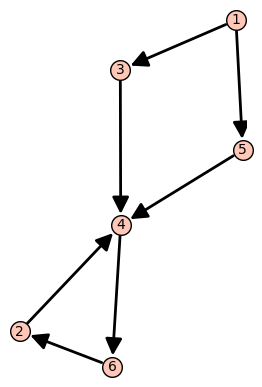
\includegraphics[width=\linewidth]{images/fig-relation-graph.png}
\end{image}%
\tcblower
\end{figureptx}%
%
\begin{enumerate}[label=(\alph*)]
\item{}Determine the adjacency matrix of \(s\).%
\item{}Use the matrix you have constructed to find the matrix of \(s^2\).%
\item{}Draw the graph defined by the matrix product and verify that it is the graph of \(s^2\).%
\item{}Determine the matrix of the transitive closure of \(s\).%
\end{enumerate}
%
\end{divisionexerciseeg}%
\end{exercisegroup}
\par\medskip\noindent
\end{exercises-subsection-numberless}
\end{sectionptx}
%
%
\typeout{************************************************}
\typeout{Section 17.2 In-Class Exercises}
\typeout{************************************************}
%
\begin{sectionptx}{In-Class Exercises}{}{In-Class Exercises}{}{}{x:section:questions-17}
%
%
%
\typeout{************************************************}
\typeout{Exercises 17.2 Exercises}
\typeout{************************************************}
%
\begin{exercises-subsection-numberless}{Exercises}{}{Exercises}{}{}{g:exercises:idm218170222560}
\par\medskip\noindent%
%
\begin{exercisegroup}
\begin{divisionexerciseeg}{1}{}{}{g:exercise:idm218170222304}%
Let \(D\) be the set of weekdays, Monday through Friday, let \(W\) be a set of employees \(\{1, 2, 3\}\) of a tutoring center, and let \(V\) be a set of computer languages for which tutoring is offered,  \(\{A(PL), B(asic), C(++), J(ava), L(isp), P(ython)\}\). We define \(s\) (schedule) from \(D\) into \(W\) by \(d s w\) if \(w\) is scheduled to work on day \(d\). We also define \(r\) from \(W\) into \(V\) by \(w r l\) if \(w\) can tutor students in language \(l\). If \(s\) and \(r\) are defined by matrices%
\par
%
\begin{equation*}
S = 
\begin{array}{cc}
& 
\begin{array}{ccc}
1 & 2 & 3 \\
\end{array}
\\
\begin{array}{c}
M \\
T \\
W \\
R \\
F \\
\end{array}
& 
\left(
\begin{array}{ccc}
1 & 0 & 1 \\
0 & 1 & 1 \\
1 & 0 & 1 \\
0 & 1 & 0 \\
1 & 1 & 0 \\
\end{array}
\right) \\
\end{array}
\textrm{ and }R=
\begin{array}{cc}
& 
\begin{array}{cccccc}
A & B & C & J & L & P \\
\end{array}
\\
\begin{array}{c}
1 \\
2 \\
3 \\
\end{array}
& \left(
\begin{array}{cccccc}
0 & 1 & 1 & 0 & 0 & 1 \\
1 & 1 & 0 & 1 & 0 & 1 \\
0 & 1 & 0 & 0 & 1 & 1 \\
\end{array}
\right) \\
\end{array}
\end{equation*}
%
\par
%
\begin{enumerate}[label=(\alph*)]
\item{}compute \(S R\) using Boolean arithmetic and give an interpretation of the relation it defines, and%
\item{}compute \(S R\) using regular arithmetic and give an interpretation of what the result describes.%
\end{enumerate}
%
\end{divisionexerciseeg}%
\begin{divisionexerciseeg}{2}{}{}{g:exercise:idm218170209872}%
Let \(A = \{a, b, c, d\}\).  Let \(r\) be the relation on \(A\) with adjacency matrix \(\begin{array}{cc}
& 
\begin{array}{cccc}
a & b & c & d \\
\end{array}
\\
\begin{array}{c}
a \\
b \\
c \\
d \\
\end{array}
& \left(
\begin{array}{cccc}
1 & 0 & 0 & 0 \\
0 & 1 & 0 & 0 \\
1 & 1 & 1 & 0 \\
0 & 1 & 0 & 1 \\
\end{array}
\right) \\
\end{array}\)%
\par
%
\begin{enumerate}[label=(\alph*)]
\item{}Explain why \(r\) is a partial ordering on \(A\).%
\item{}Draw its Hasse diagram.%
\end{enumerate}
%
\end{divisionexerciseeg}%
\begin{divisionexerciseeg}{3}{}{}{g:exercise:idm218170205360}%
What common relations on \(\mathbb{Z}\) are the transitive closures of the following relations?%
\par
%
\begin{enumerate}[label=(\alph*)]
\item{}\(a S b\) if and only if \(a + 1 = b\).%
\item{}\(a R b\) if and only if \(| a - b | = 2\).%
\end{enumerate}
%
\end{divisionexerciseeg}%
\begin{divisionexerciseeg}{4}{}{}{g:exercise:idm218170201264}%
%
\begin{enumerate}[label=(\alph*)]
\item{}Prove that if \(r\) is a transitive relation on a set \(A\), then \(r^2 \subseteq  r\).%
\item{}Find an example of a transitive relation for which \(r^2\neq r\).%
\end{enumerate}
%
\end{divisionexerciseeg}%
\end{exercisegroup}
\par\medskip\noindent
\end{exercises-subsection-numberless}
\end{sectionptx}
\end{chapterptx}
 %
%
\typeout{************************************************}
\typeout{Chapter 18 Functions and Their Properties}
\typeout{************************************************}
%
\begin{chapterptx}{Functions and Their Properties}{}{Functions and Their Properties}{}{}{x:chapter:chapter_18}
\index{Function Properties}%
%
%
\typeout{************************************************}
\typeout{Section 18.1 Reading Assignment}
\typeout{************************************************}
%
\begin{sectionptx}{Reading Assignment}{}{Reading Assignment}{}{}{x:section:reading-18}
Read Sections 7.1 and 7.2 of \emph{Applied Discrete Structures}.  You may think you know about functions if you've taken calculus, but the approach to functions in Chapter 7, which is the more formal approach, is different. So make an effort to memorize the terms!  The good news is that there are only two key properties that are introduced in Section 7.2.%
\begin{question}{Response Question.}{g:question:idm218170195424}%
In programming, a \emph{function} is a named section of a program that performs a specific task and returns a value.  How does this compare with the definition of a function in mathematics?%
\end{question}
Also, turn in solutions to these exercises:%
%
%
\typeout{************************************************}
\typeout{Exercises 18.1 Exercises}
\typeout{************************************************}
%
\begin{exercises-subsection-numberless}{Exercises}{}{Exercises}{}{}{g:exercises:idm218170193840}
\par\medskip\noindent%
%
\begin{exercisegroup}
\begin{divisionexerciseeg}{1}{}{}{g:exercise:idm218170193584}%
At the end of the semester a teacher assigns letter grades to each of her 45 students. Is this a function? If so, what sets make up the domain and codomain, and is the function injective, surjective, bijective, or neither?%
\end{divisionexerciseeg}%
\begin{divisionexerciseeg}{2}{}{}{g:exercise:idm218170192688}%
Let \(A\) be a set and let \(S\) be any subset of \(A\). Let \(\chi_S: A\to \{0,1\}\) be defined by%
\begin{equation*}
\chi_S(x)= \left\{
\begin{array}{cc}
1 & \textrm{if } x\in S \\
0 & \textrm{if } x\notin S \\
\end{array}
\right.
\end{equation*}
%
\par
The function \(\chi_S\) is called the \terminology{characteristic function}\index{Characteristic function} of \(S\).%
\par
Suppose \(A = \{a, b, c\}\).%
\begin{enumerate}[label=(\alph*)]
\item{}If  \(S = \{a, b\}\), list the elements of \(\chi_S\) .%
\item{}What are \(\chi_{\emptyset}\) and \(\chi_A\)?%
\end{enumerate}
%
\end{divisionexerciseeg}%
\end{exercisegroup}
\par\medskip\noindent
\end{exercises-subsection-numberless}
\end{sectionptx}
%
%
\typeout{************************************************}
\typeout{Section 18.2 In-Class Exercises}
\typeout{************************************************}
%
\begin{sectionptx}{In-Class Exercises}{}{In-Class Exercises}{}{}{x:section:questions-18}
%
%
%
\typeout{************************************************}
\typeout{Exercises 18.2 Exercises}
\typeout{************************************************}
%
\begin{exercises-subsection-numberless}{Exercises}{}{Exercises}{}{}{g:exercises:idm218170183312}
\par\medskip\noindent%
%
\begin{exercisegroup}
\begin{divisionexerciseeg}{1}{}{}{g:exercise:idm218170183056}%
Define functions on the positive integers, \(\mathbb{P}\), if they exist, that have the properties specified below.%
\begin{enumerate}[label=(\alph*)]
\item{}A function that is one-to-one and onto.%
\item{}A function that is neither one-to-one nor onto.%
\item{}A function that is one-to-one but not onto.%
\item{}A function that is onto but not one-to-one.%
\end{enumerate}
%
\end{divisionexerciseeg}%
\begin{divisionexerciseeg}{2}{}{}{g:exercise:idm218170179776}%
Prove that in a room with \(n\) people, \(n \geq 2\), at least two people know exactly the same number of people. Assume knowing is a symmetric relation: If Paul knows Pat, then Pat knows Paul.%
\end{divisionexerciseeg}%
\begin{divisionexerciseeg}{3}{}{}{g:exercise:idm218170178352}%
Infinite Acres Spa and Math Camp has an infinite number of single occupancy rooms, numbered with each positive integer.  You are the night manager.  The spa is fully booked for the weekend and all rooms are occupied. A bus arrives late Friday night.  You find that the manager has booked an additional infinite busload of customers, with confirmation codes numbered \(1, 2, 3, \dots\).   Can you accomodate the new arrivals?%
\end{divisionexerciseeg}%
\begin{divisionexerciseeg}{4}{}{}{g:exercise:idm218170177088}%
Prove that the set of finite strings of 0's and 1's is countable.%
\end{divisionexerciseeg}%
\end{exercisegroup}
\par\medskip\noindent
\end{exercises-subsection-numberless}
\end{sectionptx}
\end{chapterptx}
 %
%
\typeout{************************************************}
\typeout{Chapter 19 Function Composition}
\typeout{************************************************}
%
\begin{chapterptx}{Function Composition}{}{Function Composition}{}{}{x:chapter:chapter_19}
\index{Function Composition}%
%
%
\typeout{************************************************}
\typeout{Section 19.1 Reading Assignment}
\typeout{************************************************}
%
\begin{sectionptx}{Reading Assignment}{}{Reading Assignment}{}{}{x:section:reading-19}
Read Section 7.3 of \emph{Applied Discrete Structures}.  The key concept in this section is function composition, which is fundamental in mathematics and computer science. Be sure to learn how it works and you'll be in good shape for the rest of the book!%
\begin{question}{Response Question.}{g:question:idm218170173568}%
Google ``linux piping'' and describe how this technique is related to function composition.%
\end{question}
Also, turn in solutions to these exercises:%
%
%
\typeout{************************************************}
\typeout{Exercises 19.1 Exercises}
\typeout{************************************************}
%
\begin{exercises-subsection-numberless}{Exercises}{}{Exercises}{}{}{g:exercises:idm218170171568}
\par\medskip\noindent%
%
\begin{exercisegroup}
\begin{divisionexerciseeg}{1}{}{}{g:exercise:idm218170171312}%
Define \(s\), \(u\), and \(d\), all functions on the integers, by \(s(n) = n^2\) , \(u(n) = n + 1\), and \(d(n) = n-1\). Determine:%
\begin{enumerate}[label=(\alph*)]
\item{}\(\displaystyle u \circ  s \circ  d\)%
\item{}\(\displaystyle s \circ  u\circ  d\)%
\item{}\(\displaystyle d \circ  s \circ  u\)%
\end{enumerate}
Describe each function with a formula similar to the way that individual functions \(s, u \textrm{ and } d\) were defined.%
\end{divisionexerciseeg}%
\begin{divisionexerciseeg}{2}{}{}{g:exercise:idm218170170832}%
%
\begin{itemize}[label=\textbullet]
\item{}Does \(f:\mathbb{Z} \rightarrow \mathbb{Z}\) defined by \(f(x)=2x+1\) have an inverse? If it does, what is it? If it doesn't, why?%
\item{}Does \(g:\mathbb{R} \rightarrow \mathbb{R}\) defined by \(g(x)=2x+1\) have an inverse? If it does, what is it? If it doesn't, why?%
\end{itemize}
%
\end{divisionexerciseeg}%
\end{exercisegroup}
\par\medskip\noindent
\end{exercises-subsection-numberless}
\end{sectionptx}
%
%
\typeout{************************************************}
\typeout{Section 19.2 In-Class Exercises}
\typeout{************************************************}
%
\begin{sectionptx}{In-Class Exercises}{}{In-Class Exercises}{}{}{x:section:questions-19}
%
%
%
\typeout{************************************************}
\typeout{Exercises 19.2 Exercises}
\typeout{************************************************}
%
\begin{exercises-subsection-numberless}{Exercises}{}{Exercises}{}{}{g:exercises:idm218170160720}
\par\medskip\noindent%
%
\begin{exercisegroup}
\begin{divisionexerciseeg}{1}{}{}{g:exercise:idm218170160464}%
Let \(A = \{1, 2, 3, 4\}\). Define \(f:A\rightarrow A\) by \(f(1) = 2\), \(f(2) = 3\), \(f(3) = 4\), and \(f(4) = 1\). Find \(f^2\), \(f^3\), \(f^4\) and \(f^{-1}\).  You can describe each of these functions as being equal to a previous one, or in the same manner as \(f\) was originally described.%
\end{divisionexerciseeg}%
\begin{divisionexerciseeg}{2}{}{}{g:exercise:idm218170160080}%
Prove that if a function has an inverse, that inverse must be unique.%
\end{divisionexerciseeg}%
\begin{divisionexerciseeg}{3}{}{}{g:exercise:idm218170154880}%
Let \(f\) and \(g\) be functions whose inverses exist. Prove that \((f\circ g)^{-1}= g^{-1}\circ f^{-1}\).%
\end{divisionexerciseeg}%
\begin{divisionexerciseeg}{4}{}{}{g:exercise:idm218170152976}%
%
\begin{enumerate}[label=(\alph*)]
\item{}Our definition of cardinality states that two sets, \(A\) and \(B\), have the same cardinality if there exists a bijection between the two sets. Why does it not matter whether the bijection is from \(A\) into \(B\) or \(B\) into \(A\)?%
\item{}Prove that ``has the same cardinality as'' is an equivalence relation on sets.%
\end{enumerate}
%
\end{divisionexerciseeg}%
\end{exercisegroup}
\par\medskip\noindent
\end{exercises-subsection-numberless}
\end{sectionptx}
\end{chapterptx}
 %
%
\typeout{************************************************}
\typeout{Chapter 20 Recursion and Sequences}
\typeout{************************************************}
%
\begin{chapterptx}{Recursion and Sequences}{}{Recursion and Sequences}{}{}{x:chapter:chapter_20}
\index{Recursion}%
\index{Stack}%
%
%
\typeout{************************************************}
\typeout{Section 20.1 Reading Assignment}
\typeout{************************************************}
%
\begin{sectionptx}{Reading Assignment}{}{Reading Assignment}{}{}{x:section:reading-20}
Read  Sections 8.1 and 8.2 of \emph{Applied Discrete Structures}.  You will see a variety of things that are most easily described through self-reference.  Most computer languages allow recursion, which can be a powerful tool when used properly.%
\begin{question}{Response Question.}{g:question:idm218170145520}%
Recursion is used in both mathematics and computer programming. Most programming languages allow recursion and they use something called a \emph{stack} to allow a function to ``call'' itself, such as in the python definition for the \hyperref[x:section:s-bsa]{Binary Search Algorithm}.  Google "what is a stack" and briefly describe, in your own words, what you've learned.%
\end{question}
Also, turn in solutions to these exercises:%
%
%
\typeout{************************************************}
\typeout{Exercises 20.1 Exercises}
\typeout{************************************************}
%
\begin{exercises-subsection-numberless}{Exercises}{}{Exercises}{}{}{g:exercises:idm218170143392}
\par\medskip\noindent%
%
\begin{exercisegroup}
\begin{divisionexerciseeg}{1}{}{}{g:exercise:idm218170142176}%
Consider a sequence of strings, \(L(n)\) defined recursively by \(L(n)=L(n-2)+L(n-2)+L(n-1)\) with \(L(0)="1"\) and \(L(1)="0"\). Here, the plus sign is taken as concatenation of strings.  Determine \(L(4)\).%
\end{divisionexerciseeg}%
\begin{divisionexerciseeg}{2}{}{}{g:exercise:idm218170141632}%
Consider sequence \(Q\) defined by \(Q(k) = 2k + 9\), \(k \geq  1\). Complete the table below and determine a recurrence relation that describes \(Q\). \(\begin{array}{c|c|c}
k & Q(k)  & Q(k)-Q(k-1) \\
\hline
2 &   &   \\
3 &   &   \\
4 & \text{  } &   \\
5 &   &   \\
6 &   &   \\
7 &   &   \\
\end{array}\)%
\end{divisionexerciseeg}%
\end{exercisegroup}
\par\medskip\noindent
\end{exercises-subsection-numberless}
\end{sectionptx}
%
%
\typeout{************************************************}
\typeout{Section 20.2 In-Class Exercises}
\typeout{************************************************}
%
\begin{sectionptx}{In-Class Exercises}{}{In-Class Exercises}{}{}{x:section:questions-20}
%
%
%
\typeout{************************************************}
\typeout{Exercises 20.2 Exercises}
\typeout{************************************************}
%
\begin{exercises-subsection-numberless}{Exercises}{}{Exercises}{}{}{g:exercises:idm218170135584}
\par\medskip\noindent%
%
\begin{exercisegroup}
\begin{divisionexerciseeg}{1}{}{}{g:exercise:idm218170135328}%
What is computed by the following function on the natural numbers?%
\begin{equation*}
f(n)=\begin{cases} 
2 f(n-1)+1 & n \gt 0 \\
1			 & n=0
\end{cases}
\end{equation*}
%
\end{divisionexerciseeg}%
\begin{divisionexerciseeg}{2}{}{}{g:exercise:idm218170134112}%
Describe what the following function, \(f\), does on the positive integers.%
\begin{equation*}
f(n)=\begin{cases} 
n & n\textrm{ odd} \\
3\cdot f(n/2) & n\textrm{ even}
\end{cases}
\end{equation*}
%
\end{divisionexerciseeg}%
\begin{divisionexerciseeg}{3}{}{}{g:exercise:idm218170134528}%
I'm thinking of a number between 1 and 25.  If I know you will use the binary search algorithm to guess my number and I want you to use as many guesses as possible, what are the best numbers for me to think about?%
\end{divisionexerciseeg}%
\begin{divisionexerciseeg}{4}{}{}{g:exercise:idm218170131904}%
The length of a string is the number of characters in the string. Let \(v(n)\) be the length of \(L(n)\), which was defined in the the homework problems.  Find a recursive description of \(v(n)\).%
\end{divisionexerciseeg}%
\begin{divisionexerciseeg}{5}{}{}{g:exercise:idm218170130080}%
\emph{Fun Question}.  This last question comes from the BBC quiz show ``Round Britain''. I expect that you would need to Google some of these references.  If Barker and Corbett encountered, sequentially, Kieslowski's colours, Blyton's adventurers, Tarantino's undesirables and Thurber's timepieces, how many pilots would they meet next?  The answer will appear at the end of the next chapter.%
\end{divisionexerciseeg}%
\end{exercisegroup}
\par\medskip\noindent
\end{exercises-subsection-numberless}
\end{sectionptx}
%
%
\typeout{************************************************}
\typeout{Section 20.3 Binary Search Algorithm}
\typeout{************************************************}
%
\begin{sectionptx}{Binary Search Algorithm}{}{Binary Search Algorithm}{}{}{x:section:s-bsa}
\index{Binary Search}%
Here is a python version of the binary search algorithm.%
\begin{codedisplay}

def BinarySearch(r,j,k,C):
   found = False
   if j <= k:
      mid = floor((j + k)/2)
      print('probing at position '+str(mid))
      if r[mid] == C:
         location = mid
         found = True
         print('found in position '+str(location))
         return location
      else:
        if r[mid] > C:
           BinarySearch(r,j, mid - 1,C)
        else:
           BinarySearch(r,mid + 1,k,C)
   else:
      print('not found')
      return False      

\end{codedisplay}
The output from an example of a search for the number 30  in a list of 28 numbers follows. It should be noted that in python indices start at 0, so we initially look for 30 in the entries indexed from 0 to 29.  Also, probing position 13 means looking at the 14th entry in the list.%
\begin{codedisplay}

s=[1,9,13,16,30,31,32,33,36,37,38,45,49,50,52,61,63,64,69,77,79,80,81,83,86,90,93,96]
BinarySearch(s,0,len(s)-1,30)

\end{codedisplay}
Output:%
\begin{codedisplay}

probing at position 13
probing at position 6
probing at position 2
probing at position 4
found in position 4

\end{codedisplay}
%
\end{sectionptx}
\end{chapterptx}
 %
%
\typeout{************************************************}
\typeout{Chapter 21 Solving Linear Recurrence Relations I}
\typeout{************************************************}
%
\begin{chapterptx}{Solving Linear Recurrence Relations I}{}{Solving Linear Recurrence Relations I}{}{}{x:chapter:chapter_21}
\index{Homogeneous Recurrence Relations}%
%
%
\typeout{************************************************}
\typeout{Section 21.1 Reading Assignment}
\typeout{************************************************}
%
\begin{sectionptx}{Reading Assignment}{}{Reading Assignment}{}{}{x:section:reading-21}
Read the first three subsections of Section 8.3 of \emph{Applied Discrete Structures}.  This will take you up to, but not including the section titled ``Solution of Nonhomogeneous Finite Order Linear Relations''.   Again, the key is to make sure you become familiar with the terms that are introduced in this section.%
\begin{question}{Response Question.}{g:question:idm218170122064}%
One of the main reasons why recurrence relations are part of this course is that the time and\slash{}or memory needs of a computer algorithm are often measured by first identifying a recurrence relation.  Once solved, many sorting algorithm are found to take a time that is proportional to \(n^2\) to sort \(n\) items.  If you are using an algorithm of this type, and it takes three minutes to sort a file with 10 million items, how long would you expect the algorithm to take to sort 20 million items?%
\end{question}
Also, turn in solutions to these exercises:%
%
%
\typeout{************************************************}
\typeout{Exercises 21.1 Exercises}
\typeout{************************************************}
%
\begin{exercises-subsection-numberless}{Exercises}{}{Exercises}{}{}{g:exercises:idm218170120160}
\par\medskip\noindent%
%
\begin{exercisegroup}
\begin{divisionexerciseeg}{1}{}{}{g:exercise:idm218170119136}%
Find a closed form expression that for the sequence \(S(n)\) if  \(S(0)=4\) and \(S(n)=3 \cdot S(n-1)\) if \(n \gt 0\).%
\end{divisionexerciseeg}%
\begin{divisionexerciseeg}{2}{}{}{g:exercise:idm218170118832}%
Find a closed form expression that for the sequence \(T(n)\) if  \(T(0)=1\), \(T(1)= 5\) and \(T(n)- 3\cdot T(n-1) -4 \cdot T(n-2)=0\) if \(n \gt 2\).%
\end{divisionexerciseeg}%
\end{exercisegroup}
\par\medskip\noindent
\end{exercises-subsection-numberless}
\end{sectionptx}
%
%
\typeout{************************************************}
\typeout{Section 21.2 In-Class Exercises}
\typeout{************************************************}
%
\begin{sectionptx}{In-Class Exercises}{}{In-Class Exercises}{}{}{x:section:questions-21}
%
%
%
\typeout{************************************************}
\typeout{Exercises 21.2 Exercises}
\typeout{************************************************}
%
\begin{exercises-subsection-numberless}{Exercises}{}{Exercises}{}{}{g:exercises:idm218170113440}
\par\medskip\noindent%
%
\begin{exercisegroup}
\begin{divisionexerciseeg}{1}{}{}{g:exercise:idm218170113104}%
Find a closed form expression that for the sequence \(V(n)\) if  \(V(0)=2\), \(V(1)= 3\) and \(V(n)= \frac{1}{2}\cdot V(n-1)+ \frac{1}{2}\cdot V(n-2)\) if \(n \geq 2\).%
\par\smallskip%
\noindent\textbf{\blocktitlefont Answer}.\hypertarget{g:answer:idm218170112560}{}\quad{}\(V(n)=\frac{8}{3}+\frac{2}{3} (-\frac{1}{2})^{n+1}\)%
\end{divisionexerciseeg}%
\begin{divisionexerciseeg}{2}{}{}{g:exercise:idm218170110464}%
Find a closed form expression that for the sequence \(Q(n)\) if  \(Q(0)=3\), \(Q(1)= 0\) and \(Q(n)=6\cdot Q(n-1)-9\cdot Q(n-2)\) if \(n \geq 2\).%
\par\smallskip%
\noindent\textbf{\blocktitlefont Answer}.\hypertarget{g:answer:idm218170109248}{}\quad{}\(Q(n)=(1-n)3^{n+1}\)%
\end{divisionexerciseeg}%
\begin{divisionexerciseeg}{3}{}{}{g:exercise:idm218170106304}%
The recurrence relation \(R(n)=R(n-1)+2^n\), \(n \geq 1\) is non-homogeneous.  This is the subject of the next class, but it can be turned into a second order homogeneous recurrence relation.  This can be done by replacing \(n\) with \(n-1\) in the recurrence relation and multiplying that equation by 2.   You can then eliminate the \(2^n\) term. Find the general solution to the resulting second order recurrence relation.%
\end{divisionexerciseeg}%
\begin{divisionexerciseeg}{4}{}{}{g:exercise:idm218170105920}%
The \hyperref[x:section:def-fibonacci-sequence]{Fibonacci Sequence}  is a second order homogeneous linear recurrence relation. It's characteristic roots are no so nice and clean as some of the examples we've seen, but developing a closed form solution is made easier by the fact that if \(\alpha\) and \(\beta\) are its two characteristic roots, then \(\alpha + \beta = 1\) and \(\alpha \cdot \beta =-1\).  Verify this and then solve for a closed form expression for \(F_k\).%
\end{divisionexerciseeg}%
\end{exercisegroup}
\par\medskip\noindent
\end{exercises-subsection-numberless}
\end{sectionptx}
%
%
\typeout{************************************************}
\typeout{Section 21.3 Fibonacci Sequence}
\typeout{************************************************}
%
\begin{sectionptx}{Fibonacci Sequence}{}{Fibonacci Sequence}{}{}{x:section:def-fibonacci-sequence}
\index{Fibonacci Sequence}%
The Fibonacci Sequence is the sequence \(F\) defined by%
\begin{equation*}
F_0= 1 \textrm{, } F_1= 1\textrm{ and}
\end{equation*}
%
\begin{equation*}
F_k = F_{k-2} + F_{k-1} \textrm{ for }k\geq 2
\end{equation*}
%
\begin{note}{}{g:note:idm218170097408}%
Some people prefer to start the Fibonacci numbers with 0 and 1 instead of 1 and 1.  that doesn't really change the main properties of the sequence, but indices may need adjusting.%
\end{note}
Answer to the last in-class question in the previous chapter: These clues give you numbers in ascending order: The TWO Ronnies, the THREE colours trilogy, the Famous FIVE, the Hateful EIGHT, Thurber's THIRTEEN clocks. This is a Fibonacci sequence, in which each number is the sum of the previous two. The next number in the sequence (and the answer to the question) must therefore be 21 - as in the rock band, 21 Pilots. This was a question posed at the end of Programme 7 of the 2020 Round Britain Quiz.%
\end{sectionptx}
\end{chapterptx}
 %
%
\typeout{************************************************}
\typeout{Chapter 22 Solving Linear Recurrence Relations II}
\typeout{************************************************}
%
\begin{chapterptx}{Solving Linear Recurrence Relations II}{}{Solving Linear Recurrence Relations II}{}{}{x:chapter:chapter_22}
\index{}%
%
%
\typeout{************************************************}
\typeout{Section 22.1 Reading Assignment}
\typeout{************************************************}
%
\begin{sectionptx}{Reading Assignment}{}{Reading Assignment}{}{}{x:section:reading-22}
Read the remainder of Section 8.3 starting with Subsection 8.3.4: ``Solution of Nonhomogeneous Finite Order Linear Relations.''  Once you've completed this section - it's a long one - you should be able to solve many recurrence relations that appear in mathematics and computer science.   Not all of them though!%
\begin{question}{Response Question.}{g:question:idm218170093360}%
An algorithm that sorts files in ``\(n \log{n}\)-time'' is normally considered better than one that sorts in ``\(n^2\)-time''.  However, that's not always the case for smaller files.  The time it takes to sort \(n\) items using Algorithms A and B take \(1200\cdot n \log_2{n}\) nanoseconds and \(5 n^2\) nanoseconds. respectively. How large must a file be to make Algorithm A the preferred one?%
\end{question}
Also, turn in solutions to these exercises:%
%
%
\typeout{************************************************}
\typeout{Exercises 22.1 Exercises}
\typeout{************************************************}
%
\begin{exercises-subsection-numberless}{Exercises}{}{Exercises}{}{}{g:exercises:idm218170089168}
\par\medskip\noindent%
%
\begin{exercisegroup}
\begin{divisionexerciseeg}{1}{}{}{g:exercise:idm218170088912}%
Find a closed form solution to \(S(k) - 2 S (k - 1) = 5^k\), with \(S(0) = 3\)%
\end{divisionexerciseeg}%
\begin{divisionexerciseeg}{2}{}{}{g:exercise:idm218170087360}%
What form would a particular solution to \(T(n)-5\cdot T(n-1)+6\cdot T(n-2)=7 \cdot 3^n\) take?  Find just a particular solution at this time.%
\end{divisionexerciseeg}%
\end{exercisegroup}
\par\medskip\noindent
\end{exercises-subsection-numberless}
\end{sectionptx}
%
%
\typeout{************************************************}
\typeout{Section 22.2 In-Class Exercises}
\typeout{************************************************}
%
\begin{sectionptx}{In-Class Exercises}{}{In-Class Exercises}{}{}{x:section:questions-22}
%
%
%
\typeout{************************************************}
\typeout{Exercises 22.2 Exercises}
\typeout{************************************************}
%
\begin{exercises-subsection-numberless}{Exercises}{}{Exercises}{}{}{g:exercises:idm218170085648}
\par\medskip\noindent%
%
\begin{exercisegroup}
\begin{divisionexerciseeg}{1}{}{}{g:exercise:idm218170085392}%
Suppose that a computer algorithm takes no time to sort a list with one item, but if it is given a list with \(n\) items, \(n \geq 2\), then it takes \(T(n) = T(n-1) + 3\cdot n\) nanoseconds.  Find a closed form expression for \(T(n)\)%
\end{divisionexerciseeg}%
\begin{divisionexerciseeg}{2}{}{}{g:exercise:idm218170082832}%
Find a closed form solution to \(S(k) - 5S(k - 1) + 6S(k - 2) = 2\), with \(S(0) = -1\), and \(S(1) = 0\).%
\end{divisionexerciseeg}%
\begin{divisionexerciseeg}{3}{}{}{g:exercise:idm218170081008}%
Find a closed form solution to \(S(k) - 5S(k - 1) + 6S(k - 2) = 7 \cdot 3^k\), with \(S(0) = 1\), and \(S(1) = 3\).%
\end{divisionexerciseeg}%
\begin{divisionexerciseeg}{4}{}{}{g:exercise:idm218170079184}%
If you were to deposit a certain amount of money at the end of each year for a number of years, this sequence of payments would be called an \emph{annuity}.  With an annual interest rate of 5 percent, how much would you need to deposit into an annuity to have a value of one million dollars after 18 years?%
\end{divisionexerciseeg}%
\end{exercisegroup}
\par\medskip\noindent
\end{exercises-subsection-numberless}
\end{sectionptx}
%
%
\typeout{************************************************}
\typeout{Section 22.3 Interest}
\typeout{************************************************}
%
\begin{sectionptx}{Interest}{}{Interest}{}{}{x:section:handouts-22}
Interest is earned on investments by adding to the invested amount, called the \emph{principle}. An interest rate is a percentage of the principle that is earned.  For example if you invest \textdollar{}2,000 in an investment  that earns 3 percent, your interest in one year would be \(\$2,000\cdot 0.03 =\$60\).  This is added to principle.  The new principle is normally computed in one step by multiplying by \(1.03\).%
\begin{equation*}
\$2,000+ \$2,000\cdot 0.03 =\$2,000\cdot 1.03 =  \$2,060.
\end{equation*}
%
\end{sectionptx}
\end{chapterptx}
 %
%
\typeout{************************************************}
\typeout{Chapter 23 Some Common Recurrence Relations}
\typeout{************************************************}
%
\begin{chapterptx}{Some Common Recurrence Relations}{}{Some Common Recurrence Relations}{}{}{x:chapter:chapter_23}
\index{}%
%
%
\typeout{************************************************}
\typeout{Section 23.1 Reading Assignment}
\typeout{************************************************}
%
\begin{sectionptx}{Reading Assignment}{}{Reading Assignment}{}{}{x:section:reading-23}
Read Section 8.4 of \emph{Applied Discrete Structures}. There is no general method for solving all recurrence relations.  In this section we consider a few cases for which the method in Section 8.3 cannot be applied.%
\begin{question}{Response Question.}{g:question:idm218170072800}%
In this section we study algorithms for searching and sorting.  If you have data that isn't sorted, then the binary search algorithm can't be implemented and you must do a sequential search. In a sequential search your look at each item in a list until you find what you're looking for, or you reach the end of the list.  What is the average number of items you will examine in a successful, and in an unsuccessful search of a list with \(n\) items?%
\end{question}
Also, turn in solutions to these exercises:%
%
%
\typeout{************************************************}
\typeout{Exercises 23.1 Exercises}
\typeout{************************************************}
%
\begin{exercises-subsection-numberless}{Exercises}{}{Exercises}{}{}{g:exercises:idm218170070608}
\par\medskip\noindent%
%
\begin{exercisegroup}
\begin{divisionexerciseeg}{1}{}{}{g:exercise:idm218170070352}%
Prove that if \(n \geq 0\), \(\lfloor n/2\rfloor +\lceil n/2\rceil = n\).%
\end{divisionexerciseeg}%
\begin{divisionexerciseeg}{2}{}{}{g:exercise:idm218170068736}%
One derangement of \(\{1,2,3,4\}\) is 2143.  List all others.%
\end{divisionexerciseeg}%
\end{exercisegroup}
\par\medskip\noindent
\end{exercises-subsection-numberless}
\end{sectionptx}
%
%
\typeout{************************************************}
\typeout{Section 23.2 In-Class Exercises}
\typeout{************************************************}
%
\begin{sectionptx}{In-Class Exercises}{}{In-Class Exercises}{}{}{x:section:questions-23}
%
%
%
\typeout{************************************************}
\typeout{Exercises 23.2 Exercises}
\typeout{************************************************}
%
\begin{exercises-subsection-numberless}{Exercises}{}{Exercises}{}{}{g:exercises:idm218170066992}
\par\medskip\noindent%
%
\begin{exercisegroup}
\begin{divisionexerciseeg}{1}{}{}{g:exercise:idm218170066736}%
The \emph{selection sort} algorithm on a list of \(n\) proceeds first by finding the largest item in the list and placing it last, exchanging it with the \(n\)-th item, if necessary.  Then a selection sort sort of the first \(n-1\) items is conducted. Let \(C(n)\) be the number of comparisons needed to complete a selection sort of \(n\) items.   Find a recurrence relation and initial condition for \(C\) and solve it.%
\end{divisionexerciseeg}%
\begin{divisionexerciseeg}{2}{}{}{g:exercise:idm218170066192}%
Suppose \(n \geq 2\) and \(1 \leq k \leq n\).  How many permutations of \(\{1,2, \dots ,n\}\),  have the property that \(k\) is a fixed point?  The set of all such permutations is called \(U_k\) in the next problem.%
\end{divisionexerciseeg}%
\begin{divisionexerciseeg}{3}{}{}{x:exercise:p3}%
Count the number of derangements of \(\{1,2,3,4\}\) using \hyperref[x:section:s-inclusion-exclusion]{inclusion-exclusion}. Do this by counting the non-derangements in the union \(U_1 \cup U_2 \cup U_3 \cup U_4\), where \(U_k\) is the set of permutations for which \(k\) is fixed. You can subtract that result from 4!   Generalize to an arbitrary value of \(n\).%
\end{divisionexerciseeg}%
\begin{divisionexerciseeg}{4}{}{}{g:exercise:idm218170059424}%
Among all continuous functions on the interval \([0,1]\), how many are derangements in that they have no fixed points?%
\end{divisionexerciseeg}%
\end{exercisegroup}
\par\medskip\noindent
\end{exercises-subsection-numberless}
\end{sectionptx}
%
%
\typeout{************************************************}
\typeout{Section 23.3 Inclusion-Exclusion}
\typeout{************************************************}
%
\begin{sectionptx}{Inclusion-Exclusion}{}{Inclusion-Exclusion}{}{}{x:section:s-inclusion-exclusion}
Here are the two and three set Inclusion-Exclusion Laws. You'll need to generalize to four sets and later to \(n\) sets in \hyperlink{x:exercise:p3}{3}, but all of the sets are similar so it isn't as complicated a you might think.%
\begin{theorem}{Laws of Inclusion-Exclusion.}{}{x:theorem:inclusion-exclusion}%
\index{Inclusion-Exclusion, Laws of}%
Given finite sets \(A_1, A_2, A_3\), then%
\begin{enumerate}[label=(\alph*)]
\item\hypertarget{x:li:ie2}{}The Two Set Inclusion-Exclusion Law:%
\begin{equation*}
\lvert A_1 \cup A_2 \rvert =\lvert A_1 \rvert + \lvert A_2 \rvert - \lvert A_1 \cap A_2 \rvert  
\end{equation*}
%
\item\hypertarget{x:li:ie3}{}The Three Set Inclusion-Exclusion Law:%
\begin{equation*}
\begin{split}
\lvert A_1 \cup A_2 \cup A_3 \rvert & =\lvert A_1 \rvert + \lvert A_2 \rvert + \lvert A_3 \rvert\\
&\quad - (\lvert A_1 \cap A_2 \rvert + \lvert A_1 \cap A_3 \rvert+ \lvert A_2 \cap A_3 \rvert)\\
&\quad + \lvert A_1 \cap A_2 \cap A_3 \rvert
\end{split} 
\end{equation*}
%
\end{enumerate}
%
\end{theorem}
\end{sectionptx}
\end{chapterptx}
 %
%
\typeout{************************************************}
\typeout{Chapter 24 Generating Functions}
\typeout{************************************************}
%
\begin{chapterptx}{Generating Functions}{}{Generating Functions}{}{}{x:chapter:chapter_24}
\index{}%
%
%
\typeout{************************************************}
\typeout{Section 24.1 Reading Assignment}
\typeout{************************************************}
%
\begin{sectionptx}{Reading Assignment}{}{Reading Assignment}{}{}{x:section:reading-24}
Read the first two subsections of Section 8.5 of \emph{Applied Discrete Structures}. Generating functions can serve as an alternative to the algorithm we introduced in Section 8.3, but also is a tool for solving other problems.%
\begin{question}{Response Question.}{g:question:idm218170045632}%
(adopteds from \hyperlink{x:biblio:biblio-bogart-2017}{[{\xreffont 1}]}) Suppose we treat addition as logical \emph{or} and multiplication as logical \emph{and}.  Furthermore, suppose that \(B\) stands for banana.  Then to say you could have as many as two bananas, we could write \(B^0+B^1+B^2=1+B+B^2\).  Suppose that in addition you could have up to three apples (use \(A\) for apples) and zero or one pears (use \(P\) for pears).  What algebraic expression represents all your choices in selecting fruits?  Identify the part of this expression where you select exactly two pieces of fruit.%
\end{question}
Also, turn in solutions to these exercises:%
%
%
\typeout{************************************************}
\typeout{Exercises 24.1 Exercises}
\typeout{************************************************}
%
\begin{exercises-subsection-numberless}{Exercises}{}{Exercises}{}{}{g:exercises:idm218170041760}
\par\medskip\noindent%
%
\begin{exercisegroup}
\begin{divisionexerciseeg}{1}{}{}{g:exercise:idm218170040688}%
What sequence has as its generating function \(\frac{1}{3-2x}\)?%
\end{divisionexerciseeg}%
\begin{divisionexerciseeg}{2}{}{}{g:exercise:idm218170039472}%
How are the generating functions of the sequences \(S(n)=n^2\) and \(T(n)=(n+1)^2\) related?%
\end{divisionexerciseeg}%
\end{exercisegroup}
\par\medskip\noindent
\end{exercises-subsection-numberless}
\end{sectionptx}
%
%
\typeout{************************************************}
\typeout{Section 24.2 In-Class Exercises}
\typeout{************************************************}
%
\begin{sectionptx}{In-Class Exercises}{}{In-Class Exercises}{}{}{x:section:questions-24}
%
%
%
\typeout{************************************************}
\typeout{Exercises 24.2 Exercises}
\typeout{************************************************}
%
\begin{exercises-subsection-numberless}{Exercises}{}{Exercises}{}{}{g:exercises:idm218170037504}
\par\medskip\noindent%
%
\begin{exercisegroup}
\begin{divisionexerciseeg}{1}{}{}{g:exercise:idm218170037248}%
Let%
\begin{equation*}
d(n)=
\begin{cases}
1 & \textrm{if }1 \leq n \leq 6\\
0 & \textrm{if }n=0\textrm{ or }n \gt 6
\end{cases}.
\end{equation*}
What sequence has as its generating function \(G(d;z)^2\)?  How is that sequence related to what you get when you roll two dice and add the top faces?%
\end{divisionexerciseeg}%
\begin{divisionexerciseeg}{2}{}{}{g:exercise:idm218170035440}%
Earlier, we proved that with supplies of five and eight cent stamps, we could make any postage amount of 28 cents or more.  Here, we will look at what smaller amounts can and can't be made.  Let \(F(z)= \sum_{n=0}^{\infty} (z^{5})^n\) and \(E(z)=\sum_{n=0}^{\infty} (z^{8})^n\).  Every combination of stamps corresponds with the product of one term from \(F(z)\) with one term from \(E(z)\).  For example, the product \((z^{5})^{2}\cdot (z^{8})^1= z^{18}\)  corresponds with combining two five cent stamps and one eight cent stamp.  Compute the first few terms of \(F(z)\cdot E(z)\) to  get all terms with degree less than 28. The terms that are missing (have a coefficient of zero) are the ones that correspond with amounts that can't be created.  In general, the coefficient of \(z^n\) in the product will be the number of ways that \(n\) cents can be made. Do a similar calculation to identify the amounts that cannot created with 7 and 9 cent stamps.%
\end{divisionexerciseeg}%
\begin{divisionexerciseeg}{3}{}{}{g:exercise:idm218170034960}%
How many ways can you give someone fifty cents using any number of nickels, dimes, and quarters?%
\end{divisionexerciseeg}%
\end{exercisegroup}
\par\medskip\noindent
\end{exercises-subsection-numberless}
\end{sectionptx}
\end{chapterptx}
\end{partptx}
%
%
\typeout{************************************************}
\typeout{Part II Structures}
\typeout{************************************************}
%
\begin{partptx}{Structures}{}{Structures}{}{}{g:part:idm218170761568}
 %
%
\typeout{************************************************}
\typeout{Chapter 25 Start of Second Semeser, Review}
\typeout{************************************************}
%
\begin{chapterptx}{Start of Second Semeser, Review}{}{Start of Second Semeser, Review}{}{}{x:chapter:chapter_101}
\begin{introduction}{}%
In the first class of the second semester, some time will be taken to review the course format and syllabus.  In the remaining time, work on problems that review some of the fundamental concepts from the first semester.%
\end{introduction}%
%
%
\typeout{************************************************}
\typeout{Section 25.1 In-Class Exercises}
\typeout{************************************************}
%
\begin{sectionptx}{In-Class Exercises}{}{In-Class Exercises}{}{}{x:section:questions-101}
%
%
%
\typeout{************************************************}
\typeout{Exercises 25.1 Exercises}
\typeout{************************************************}
%
\begin{exercises-subsection-numberless}{Exercises}{}{Exercises}{}{}{g:exercises:idm218170027344}
\par\medskip\noindent%
%
\begin{exercisegroup}
\begin{divisionexerciseeg}{1}{}{}{g:exercise:idm218170027008}%
Prove that if \(f\) and \(g\) are bijections on a set \(X\), then \(g \circ f\) is also a bijection on \(X\).%
\end{divisionexerciseeg}%
\begin{divisionexerciseeg}{2}{}{}{g:exercise:idm218170026464}%
Partition the set \(X=\{k \in \mathbb{Z} \mid  -10 \leq k \leq 10\}\) into equivalence classes according to the relation congruence modulo 4, \(\equiv_4\).%
\end{divisionexerciseeg}%
\begin{divisionexerciseeg}{3}{}{}{g:exercise:idm218170022560}%
Is the following logical argument valid?%
\begin{quote}%
Peacham is either in Vermont or New Hampshire. If Peacham is in Vermont, then Peacham is in New England. If Peacham is in New Hamphire, then Peacham is in New England. Therefore, Peacham is in New England.%
\end{quote}
\par\smallskip%
\noindent\textbf{\blocktitlefont Answer}.\hypertarget{g:answer:idm218170022048}{}\quad{}Yes, this argument is valid.  Symbolically, it is%
\begin{equation*}
V \lor NH, V\rightarrow NE, NH\rightarrow NE \Rightarrow NE
\end{equation*}
which can be proven correct.%
\end{divisionexerciseeg}%
\begin{divisionexerciseeg}{4}{}{}{g:exercise:idm218170020448}%
Prove, by mathematical induction, that \(F_0 + F_1 + F_2 + \cdots + F_{n} = F_{n+2} - 1\), where \(F_n\) is the \(n\)th number in the \hyperref[x:section:def-fibonacci-sequence]{Fibonacci Sequence}.%
\end{divisionexerciseeg}%
\begin{divisionexerciseeg}{5}{}{}{g:exercise:idm218170017920}%
Prove that if \(n\) is an integer and you divide \(n^2\) by 5, then the remainder is always 0, 1, or 4.%
\end{divisionexerciseeg}%
\begin{divisionexerciseeg}{6}{}{}{g:exercise:idm218170016464}%
Prove that the square root of 5 is an irrational number.%
\end{divisionexerciseeg}%
\end{exercisegroup}
\par\medskip\noindent
\end{exercises-subsection-numberless}
\end{sectionptx}
\end{chapterptx}
 %
%
\typeout{************************************************}
\typeout{Chapter 26 Graphs}
\typeout{************************************************}
%
\begin{chapterptx}{Graphs}{}{Graphs}{}{}{x:chapter:chapter_102}
\index{Graphs}%
%
%
\typeout{************************************************}
\typeout{Section 26.1 Reading Assignment}
\typeout{************************************************}
%
\begin{sectionptx}{Reading Assignment}{}{Reading Assignment}{}{}{x:section:reading-102}
Read Section 9.1 of \emph{Applied Discrete Structures}. This section introduces some basic terminology and properties of graphs.%
\begin{question}{Response Question.}{g:question:idm218170013680}%
The original version of the computer language BASIC on Apple II computers used 16 bits for an integer, one of which was used to specify the sign of the integer.  What would have been the maximum size of an integer in that language?%
\end{question}
Also, turn in solutions to these exercises:%
\begin{itemize}[label=\textbullet]
\item{}Why is the sum of the degrees of the vertices of any undirected graph always even?%
\item{}Demonstrate that \((4,3,2,2,1)\) is a graphic sequence.%
\end{itemize}
%
\end{sectionptx}
%
%
\typeout{************************************************}
\typeout{Section 26.2 In-Class Exercises}
\typeout{************************************************}
%
\begin{sectionptx}{In-Class Exercises}{}{In-Class Exercises}{}{}{x:section:questions-102}
%
\begin{enumerate}[label=\arabic*.]
\item{}Prove that any graph with at least two vertices must have two vertices of the same degree.%
\item{}Starting at vertex \(s\), any finite path in \hyperref[x:figure:fig-directed-graph-ex1]{Figure~{\xreffont\ref{x:figure:fig-directed-graph-ex1}}} produces a string of bits that are recorded according to the labels on each edge.  For example, the path \(s,a,b,a,b,b,a\) will produce the string 101001.%
\begin{figureptx}{A model for bit strings with no consecutive 1's}{x:figure:fig-directed-graph-ex1}{}%
\begin{image}{0.15}{0.7}{0.15}%
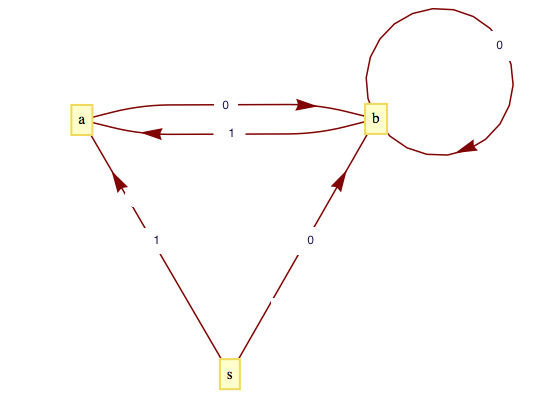
\includegraphics[width=\linewidth]{images/fig-directed-graph-ex1.png}
\end{image}%
\tcblower
\end{figureptx}%
This graph produces bit strings that contain no consecutive 1's.   Draw a graph similar to it that produces bit strings containing no more than two consecutive 1's.%
\item{}Find two isomorphisms between the following graphs.%
\begin{figureptx}{Two Isomorphic Graphs}{x:figure:fig-graphpair}{}%
\begin{image}{0.15}{0.7}{0.15}%
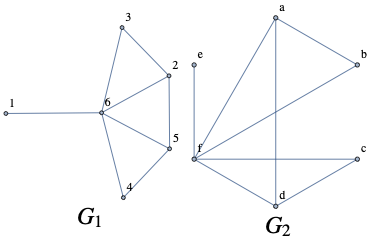
\includegraphics[width=\linewidth]{images/fig-graphpair.png}
\end{image}%
\tcblower
\end{figureptx}%
\item{}%
\begin{enumerate}[label=(\alph*)]
\item{}Determine whether the following sequences are graphic. Explain your logic if the answer is ``no'' and draw a graph with the sequence as its degree sequence if it is ``yes.''%
\begin{enumerate}[label=\roman*]
\item{}\(\displaystyle (5,1,1,1,1,1)\)%
\item{}\(\displaystyle (3,3,3,3)\)%
\item{}\(\displaystyle (3,3,3,3,3)\)%
\item{}\(\displaystyle (4,3,2,1,0)\)%
\item{}\(\displaystyle (2,2,2,1,1)\)%
\item{}\(\displaystyle (3,2,2,2,1)\)%
\end{enumerate}
%
\item{}Based on observations you might have made in from the examples above, describe as many characteristics as you can about graphic sequences.%
\end{enumerate}
%
\end{enumerate}
%
\end{sectionptx}
\end{chapterptx}
 %
%
\typeout{************************************************}
\typeout{Chapter 27 Data Structures and Connectivity}
\typeout{************************************************}
%
\begin{chapterptx}{Data Structures and Connectivity}{}{Data Structures and Connectivity}{}{}{x:chapter:chapter_103}
\index{}%
%
%
\typeout{************************************************}
\typeout{Section 27.1 Reading Assignment}
\typeout{************************************************}
%
\begin{sectionptx}{Reading Assignment}{}{Reading Assignment}{}{}{x:section:reading-103}
Read Sections 9.2 and 9.3 of \emph{Applied Discrete Structures}. The topics in these sections are data structures for graphs and connectivity between vertices in a graph.%
\begin{question}{Response Question.}{g:question:idm218169989968}%
You're certainly more familiar with the terms diameter, radius and center as they pertain to circles.  Compare their use for circles with their use in graph theory.   How are they similar and how are they different?%
\end{question}
Also, turn in solutions to these exercises:%
%
%
\typeout{************************************************}
\typeout{Exercises 27.1 Exercises}
\typeout{************************************************}
%
\begin{exercises-subsection-numberless}{Exercises}{}{Exercises}{}{}{g:exercises:idm218169988720}
\par\medskip\noindent%
%
\begin{exercisegroup}
\begin{divisionexerciseeg}{1}{}{}{g:exercise:idm218169988464}%
Draw the undirected graph that is represented by the following SageMath expression. \mono{Graph(\{1:[2,3,4],2:[3,5],3:[5,7],4:[6,7]\})}%
\end{divisionexerciseeg}%
\begin{divisionexerciseeg}{2}{}{}{g:exercise:idm218169987520}%
In a breadth first search starting at vertex 2 of the graph in the previous problem, what would be the depth sets?%
\end{divisionexerciseeg}%
\end{exercisegroup}
\par\medskip\noindent
\end{exercises-subsection-numberless}
\end{sectionptx}
%
%
\typeout{************************************************}
\typeout{Section 27.2 In-Class Exercises}
\typeout{************************************************}
%
\begin{sectionptx}{In-Class Exercises}{}{In-Class Exercises}{}{}{x:section:questions-103}
%
%
%
\typeout{************************************************}
\typeout{Exercises 27.2 Exercises}
\typeout{************************************************}
%
\begin{exercises-subsection-numberless}{Exercises}{}{Exercises}{}{}{g:exercises:idm218169986176}
\par\medskip\noindent%
%
\begin{exercisegroup}
\begin{divisionexerciseeg}{1}{}{}{g:exercise:idm218169985920}%
Determine the eccentricities of each vertex, and the diameter, radius, and center of the graph in exercise 1 of the reading assignment.%
\end{divisionexerciseeg}%
\begin{divisionexerciseeg}{2}{}{}{g:exercise:idm218169985168}%
Determine the diameter, radius, and center of the graph with the following distance matrix, where \(D_{i,j}\) is the length of the shortest path from \(i\) to \(j\).%
\begin{equation*}
D=\left(
\begin{array}{cccccccccccc}
0 & 2 & 2 & 2 & 3 & 1 & 1 & 3 & 3 & 1 & 2 & 2 \\
2 & 0 & 3 & 3 & 2 & 2 & 1 & 4 & 1 & 2 & 2 & 1 \\
2 & 3 & 0 & 2 & 5 & 3 & 2 & 3 & 4 & 1 & 4 & 3 \\
2 & 3 & 2 & 0 & 3 & 1 & 2 & 1 & 3 & 1 & 2 & 3 \\
3 & 2 & 5 & 3 & 0 & 2 & 3 & 4 & 1 & 4 & 1 & 3 \\
1 & 2 & 3 & 1 & 2 & 0 & 1 & 2 & 2 & 2 & 1 & 2 \\
1 & 1 & 2 & 2 & 3 & 1 & 0 & 3 & 2 & 1 & 2 & 1 \\
3 & 4 & 3 & 1 & 4 & 2 & 3 & 0 & 4 & 2 & 3 & 4 \\
3 & 1 & 4 & 3 & 1 & 2 & 2 & 4 & 0 & 3 & 1 & 2 \\
1 & 2 & 1 & 1 & 4 & 2 & 1 & 2 & 3 & 0 & 3 & 2 \\
2 & 2 & 4 & 2 & 1 & 1 & 2 & 3 & 1 & 3 & 0 & 3 \\
2 & 1 & 3 & 3 & 3 & 2 & 1 & 4 & 2 & 2 & 3 & 0 \\
\end{array}
\right)
\end{equation*}
Can you construct the graph from this matrix?%
\par\smallskip%
\noindent\textbf{\blocktitlefont Answer}.\hypertarget{g:answer:idm218169982080}{}\quad{}The diameter is 5, the radius is 3, and the center is \(\{4,11\}\).%
\end{divisionexerciseeg}%
\begin{divisionexerciseeg}{3}{}{}{x:exercise:class-grid-problem}%
A classroom has 5 rows of desks, with 7 desks in each row.   Suppose we want to represent this rectangular arrangement of desks in an undirected graph, where each desk is connected to the neighboring desks to it's front, back, left and right.  Of course, some desks have fewer than four neighbors.%
\begin{enumerate}[label=(\alph*)]
\item{}How many edges will the graph have?%
\item{}Determine the possible eccentricities of vertices in this graph. What is the diameter, radius and center of the graph.%
\item{}If an adjacency matrix is constructed for this graph with one bit (0\slash{}1) for each entry, how many bits would be needed?  Assume we only store the part of the matrix that appears to the top right of the main diagonal of the matrix since its symmetric.%
\item{}If an edge dictionary is used in which eight bits are used for each vertex number and eight bits for each entry in the list of adjacent vertices, how many bits would be needed? Assume that if \(i\) appears in the list of neighbors of \(j\), then we don't need to list \(j\) in the list of neighbors of \(i\).%
\item{}If a list of ordered pairs is used, where each pair requires 16 bit, how many bits would be needed?  Assume that for any two vertices, \(i\) and \(j\), only one of the pairs \((i,j)\) and \((j,i)\) need to be listed.%
\end{enumerate}
%
\par\smallskip%
\noindent\textbf{\blocktitlefont Answer}.\hypertarget{g:answer:idm218169973136}{}\quad{}%
\begin{enumerate}[label=(\alph*)]
\item{}There are \(4\cdot 7\cdot 5- 2\cdot7 - 2 \cdot 5= 116\) edges.%
\item{}Clearly the longest distance between pairs of desks is \(4+6= 10\). The shortest longest distance from any desk is 5, which is the distance from the desk in the middle of the room, the fourth desk in row 3.  There are vertices with eccentricities for all integers between 5 and 10.  The radius is 5 and the diameter is 10.   The center contains only one desk, the middle one.%
\item{}If an adjacency matrix is constructed for this graph with one bit (0\slash{}1) for each entry, how many bits would be needed?  Assume we only store the part of the matrix that appears to the top right of the main diagonal of the matrix since its symmetric.%
\item{}If an edge dictionary is used in which eight bits are used for each vertex number and eight bits for each entry in the list of adjacent vertices, how many bits would be needed? Assume that if \(i\) appears in the list of neighbors of \(j\), then we don't need to list \(j\) in the list of neighbors of \(i\).%
\item{}If a list of ordered pairs is used, where each pair requires 16 bit, how many bits would be needed?  Assume that for any two vertices, \(i\) and \(j\), only one of the pairs \((i,j)\) and \((j,i)\) need to be listed.%
\end{enumerate}
%
\end{divisionexerciseeg}%
\end{exercisegroup}
\par\medskip\noindent
\end{exercises-subsection-numberless}
\end{sectionptx}
\end{chapterptx}
 %
%
\typeout{************************************************}
\typeout{Chapter 28 Graph Traversals}
\typeout{************************************************}
%
\begin{chapterptx}{Graph Traversals}{}{Graph Traversals}{}{}{x:chapter:chapter_104}
\index{}%
%
%
\typeout{************************************************}
\typeout{Section 28.1 Reading Assignment}
\typeout{************************************************}
%
\begin{sectionptx}{Reading Assignment}{}{Reading Assignment}{}{}{x:section:reading-104}
Read Section 9.4 of \emph{Applied Discrete Structures}.  In this section, we consider whether certain paths or circuits exist in a given graph.  Our objective will either be to trace every edge once or visit every vertex once.%
\begin{question}{Response Question.}{g:question:idm218169962832}%
In the 18th century, Koenigsberg was  part of Prussia. In what country is it now? Besides its bridges, find one other fact about Koenigsberg.%
\end{question}
Also, turn in solutions to these exercises:%
%
%
\typeout{************************************************}
\typeout{Exercises 28.1 Exercises}
\typeout{************************************************}
%
\begin{exercises-subsection-numberless}{Exercises}{}{Exercises}{}{}{g:exercises:idm218169961664}
\par\medskip\noindent%
%
\begin{exercisegroup}
\begin{divisionexerciseeg}{1}{}{}{g:exercise:idm218169961408}%
In answering the question ``Is every Eulerian graph also Hamiltonian?'' Hansel pointed out an Eulerian circuit in a specific graph that visited several vertices more than once.  He concluded that this graph can't be Hamiltonian since a Hamiltonian circuit visits each vertex exactly once. Therefore, the answer to the question is ``No!'' Is his answer correct? Is his reasoning correct?  Explain your answers.%
\par\smallskip%
\noindent\textbf{\blocktitlefont Solution}.\hypertarget{g:solution:idm218169959744}{}\quad{}%
\end{divisionexerciseeg}%
\begin{divisionexerciseeg}{2}{}{}{g:exercise:idm218169959408}%
How many different Hamiltonian circuits are there of a \(K_n\), \(k \geq 3\), that start with the edge \((1,2)\)?%
\par\smallskip%
\noindent\textbf{\blocktitlefont Solution}.\hypertarget{g:solution:idm218169957456}{}\quad{}There are \((n-2)!\) circuits as described.%
\end{divisionexerciseeg}%
\end{exercisegroup}
\par\medskip\noindent
\end{exercises-subsection-numberless}
\end{sectionptx}
%
%
\typeout{************************************************}
\typeout{Section 28.2 In-Class Exercises}
\typeout{************************************************}
%
\begin{sectionptx}{In-Class Exercises}{}{In-Class Exercises}{}{}{x:section:questions-104}
%
%
%
\typeout{************************************************}
\typeout{Exercises 28.2 Exercises}
\typeout{************************************************}
%
\begin{exercises-subsection-numberless}{Exercises}{}{Exercises}{}{}{g:exercises:idm218169955872}
\par\medskip\noindent%
%
\begin{exercisegroup}
\begin{divisionexerciseeg}{1}{}{}{g:exercise:idm218169955616}%
For each of the following sets of twelve dominos, is it possible to arrange them end-to-end so that the numbers every two touching ends have matching numbers?%
\begin{enumerate}[label=(\alph*)]
\item{}\begin{figureptx}{}{g:figure:idm218169954128}{}%
\begin{image}{0}{1}{0}%
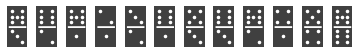
\includegraphics[width=\linewidth]{images/dominos1.png}
\end{image}%
\tcblower
\end{figureptx}%
%
\item{}\begin{figureptx}{}{g:figure:idm218169952448}{}%
\begin{image}{0}{1}{0}%
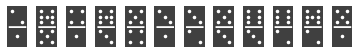
\includegraphics[width=\linewidth]{images/dominos2.png}
\end{image}%
\tcblower
\end{figureptx}%
%
\end{enumerate}
%
\par\smallskip%
\noindent\textbf{\blocktitlefont Solution}.\hypertarget{g:solution:idm218169952032}{}\quad{}The answers to both parts can be arrived at by realizing that each domino can be thought of as an edge between vertices having the two numbers on the domino.  We are then asking for an Eulerian circuit or path in the corresponding graph.  A circuit exists  for the first set of dominos, but not the second. For the second, the degrees of four vertices are odd and so the dominos cannot be arranged as desired.%
\end{divisionexerciseeg}%
\begin{divisionexerciseeg}{2}{}{}{g:exercise:idm218169950464}%
A telephone company employee needs to check the telephone lines hanging from telephone poles for a cut in the line over a grid of streets in a city without service.  What graph theory problem is she going to have to solve if she wants to do this efficiently?%
\par\smallskip%
\noindent\textbf{\blocktitlefont Solution}.\hypertarget{g:solution:idm218169949680}{}\quad{}%
\end{divisionexerciseeg}%
\begin{divisionexerciseeg}{3}{}{}{g:exercise:idm218169949424}%
King Arthur and his knights are either friends with one another or are enemies.  He has called a meeting of all of his knights and would like to have them seated at his huge round table so that each knight is seated next to two friends. What graph theory problem is he going to have to solve?%
\par\smallskip%
\noindent\textbf{\blocktitlefont Solution}.\hypertarget{g:solution:idm218169948608}{}\quad{}%
\end{divisionexerciseeg}%
\begin{divisionexerciseeg}{4}{}{}{g:exercise:idm218169948352}%
The Gray code for the 3-cube is not unique in that there are other Hamiltonian circuits that are not equal to \(G_3\) or its reverse.  Find one.   Is it your different in ``shape'' from \(G\)?   For the \(n\)-cube, \(n \gt 3\), are there Hamiltonian paths that are different in shape from \(G_n\)?%
\par\smallskip%
\noindent\textbf{\blocktitlefont Solution}.\hypertarget{g:solution:idm218169947968}{}\quad{}%
\end{divisionexerciseeg}%
\begin{divisionexerciseeg}{5}{}{}{g:exercise:idm218169945136}%
Assume we number positions in the Gray Code \(G_n\) from 0 to \(2^n-1\).  What is the bit string of in position 20 in the Gray code for the 6-cube? Where will you find 000101 in \(G_6\)?	 In what position in \(G_{10}\) will you find 0010010000?%
\par\smallskip%
\noindent\textbf{\blocktitlefont Solution}.\hypertarget{g:solution:idm218169942912}{}\quad{}%
\end{divisionexerciseeg}%
\end{exercisegroup}
\par\medskip\noindent
\end{exercises-subsection-numberless}
\end{sectionptx}
\end{chapterptx}
 %
%
\typeout{************************************************}
\typeout{Chapter 29 Planarity and Graph Coloring}
\typeout{************************************************}
%
\begin{chapterptx}{Planarity and Graph Coloring}{}{Planarity and Graph Coloring}{}{}{x:chapter:chapter_104a}
\index{Planarity}%
\index{Graph Coloring}%
\index{Chromatic Polynomial}%
%
%
\typeout{************************************************}
\typeout{Section 29.1 Reading Assignment}
\typeout{************************************************}
%
\begin{sectionptx}{Reading Assignment}{}{Reading Assignment}{}{}{x:section:reading-104a}
Read Section 9.6 of \emph{Applied Discrete Structures}. There are two main topics of this section. The first is planarity of graphs, whether a graph can be drawn on paper without having any edges crossing one another.  The second is coloring, the vertices of a graph are assigned colors with the rule that two vertices that are connected by an edge must have different colors.  The two topics are unified by the Four Color Theorem.%
\begin{question}{Response Question.}{g:question:idm218169939184}%
Who was István Fáry and what did he prove about planar graphs?%
\end{question}
Also, turn in solutions to these exercises:%
%
%
\typeout{************************************************}
\typeout{Exercises 29.1 Exercises}
\typeout{************************************************}
%
\begin{exercises-subsection-numberless}{Exercises}{}{Exercises}{}{}{g:exercises:idm218169937648}
\par\medskip\noindent%
%
\begin{exercisegroup}
\begin{divisionexerciseeg}{1}{}{}{g:exercise:idm218169937312}%
Although a \(K_{3,3}\) it is not planar, it can be embedded on a torus without any edge crossings.  This is demonstrated in the video \href{https://www.youtube.com/watch?v=k2O0Av_8_fo}{https:\slash{}\slash{}www.youtube.com\slash{}watch?v=k2O0Av\textunderscore{}8\textunderscore{}fo}.  Watch the video and then dermine whether you can embed a \(K_5\) on a torus without any edge crossings.%
\par\smallskip%
\noindent\textbf{\blocktitlefont Solution}.\hypertarget{g:solution:idm218169934752}{}\quad{}\textunderscore{}%
\end{divisionexerciseeg}%
\begin{divisionexerciseeg}{2}{}{}{g:exercise:idm218169934368}%
Find a coloring of the following graph with as few colors as possible.  Use the letters \(A,B,C,  \dots\)\textgreater{} for colors and submit your answer in the form of a partition of \(\{1,2,\dots, 8\}\):%
\begin{equation*}
\{\textrm{set of vertices with color }A, \textrm{set of vertices with color }B, \dots\}
\end{equation*}
%
\begin{sidebyside}{2}{0}{0}{0}%
\begin{sbspanel}{0.5}%
\begin{figureptx}{}{x:figure:fig-colorme-1}{}%
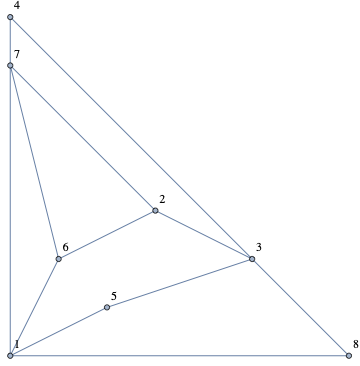
\includegraphics[width=\linewidth]{images/fig-colorme-1.png}
\tcblower
\end{figureptx}%
\end{sbspanel}%
\begin{sbspanel}{0.5}%
%
\begin{equation*}
\begin{array}{cccccccc}
1 & 2 & 3 & 4 & 5 & 6 & 7 & 8 \\
\_\_ & \_\_ & \_\_ & \_\_ & \_\_ &
\_\_ & \_\_ & \_\_ \\
\end{array}
\end{equation*}
%
\end{sbspanel}%
\end{sidebyside}%
\par\smallskip%
\noindent\textbf{\blocktitlefont Solution}.\hypertarget{g:solution:idm218169929952}{}\quad{}%
\end{divisionexerciseeg}%
\end{exercisegroup}
\par\medskip\noindent
\end{exercises-subsection-numberless}
\end{sectionptx}
%
%
\typeout{************************************************}
\typeout{Section 29.2 In-Class Exercises}
\typeout{************************************************}
%
\begin{sectionptx}{In-Class Exercises}{}{In-Class Exercises}{}{}{x:section:questions-104a}
%
%
%
\typeout{************************************************}
\typeout{Exercises 29.2 Exercises}
\typeout{************************************************}
%
\begin{exercises-subsection-numberless}{Exercises}{}{Exercises}{}{}{g:exercises:idm218169928864}
\par\medskip\noindent%
%
\begin{exercisegroup}
\begin{divisionexerciseeg}{1}{}{}{g:exercise:idm218169928608}%
If a planar graph \(G\) with 12 vertices divides the plane into 21 regions, how many edges must \(G\) have?%
\par\smallskip%
\noindent\textbf{\blocktitlefont Solution}.\hypertarget{g:solution:idm218169927248}{}\quad{}Using Euler's formula, since \(v+r-e=12+21-e=2\), \(e=31\)%
\end{divisionexerciseeg}%
\begin{divisionexerciseeg}{2}{}{}{g:exercise:idm218169926016}%
\index{Cubic Graph}%
The graph \(G\) has vertices with degree sequence \((5, 3, 3, 2, 2, 1)\). How many edges does it have? If it is planar, into how many regions of the plane does it divide?  Does \(G\) have an Eulerian path?%
\par\smallskip%
\noindent\textbf{\blocktitlefont Answer}.\hypertarget{g:answer:idm218169923824}{}\quad{}The degree sequence indicates that \(v=6\) and \(e=8\). Since \(v +r - e=6+r-8=2\), \(r = 4\).%
\end{divisionexerciseeg}%
\begin{divisionexerciseeg}{3}{}{}{g:exercise:idm218169921648}%
Suppose an undirected planar graph \(G\) has the following properties:%
\begin{itemize}[label=\textbullet]
\item{}All vertices have degree three (this called a \terminology{cubic graph})%
\item{}All faces of the graph's planar embedding are hexagons and pentagons; i. e, they is made up of either five or six edges.%
\end{itemize}
What can be said about the numbers of hexagons and pentagons in the graph?%
\par\smallskip%
\noindent\textbf{\blocktitlefont Answer}.\hypertarget{g:answer:idm218169918864}{}\quad{}There must be 12 pentagons. The number of hexagons cannot be determined.%
\end{divisionexerciseeg}%
\begin{divisionexerciseeg}{4}{}{}{g:exercise:idm218169918480}%
A teacher decides to have their students grade one another's quizzes.  The scheme that is devised is that when a bell is rung, each  student is to immediately pass their quiz to a classmate either to the front, back, right or left of themselves.  Suppose that class is arranged in rectanglar configuration of five rows of seven students each. Is is possible for each student to get exactly one quiz to grade?%
\par\smallskip%
\noindent\textbf{\blocktitlefont Solution}.\hypertarget{g:solution:idm218169917552}{}\quad{}It is not possible to arrange grading as described.  If you color the desks in the class like a checkerboard, alternating black and white desks, there will be more of one color, say white, than black. Every white desk has to pass their paper to a different black desk, but that's impossible because there aren't enough black desks.%
\end{divisionexerciseeg}%
\begin{divisionexerciseeg}{5}{}{}{g:exercise:idm218169916832}%
\index{chromatic polynomial of a graph}%
The chromatic polynomial of a graph, \(G\) is a polynomial \(g(x)\) such that for each positive integer \(n\), \(g(n)\) equals the number of different ways you can color \(G\) with \(n\) colors.  For example, the chromatic polynomial of a \(K_3\) is \(x(x-1)(x-2)\).%
\begin{enumerate}[label=(\alph*)]
\item{}What is the chromatic polynomial of a \(K_4\)?%
\item{}What is the chromatic polynomial of a \(C_4\), a cycle with four vertices?%
\item{}What is the chromatic polynomial of a \(K_{3,3}\)?%
\item{}How are the chromatic number and the chromatic polynomial of a graph related?%
\end{enumerate}
%
\par\smallskip%
\noindent\textbf{\blocktitlefont Solution}.\hypertarget{g:solution:idm218169916192}{}\quad{}%
\begin{enumerate}[label=(\alph*)]
\item{}The chromatic polynomial of a \(K_4\) is \(x(x-1)(x-2)(x-3)\). This follows from the fact that each vertex must be colored differently.%
\item{}The chromatic polynomial of a \(C_4\) is a bit more difficult to determine.   If we number the vertices 1 through 4 and start be coloring vertex 1, it can colored \(x\) ways.  Then going around a cycle of any length we color the next vertex so as to differ from the previous one.  However we run into a problem when we reach the last two vertices before reaching the start of the cycle.  For the \(4\)-cycle, vertex 1 can be colored \(x\) ways and vertex 2 can be colored \(x-1\) ways. We need to to partition the possibilities according to whether vertex 3 has the same color as vertex 1 or a different color.  If they have the same color, then there are \(x-1\) ways to color vertex 4.  If they differ in color, then there are \(x-2\) ways to color vertex 3, and then \(x-2\) ways to finish up coloring vertex 4. Therefore the chromatic polynomial is \(x(x-1)((x-1)+(x-2)^2)= x(x-1)(x^2-3x+3)\).%
\item{}The chromatic polynomial of a \(K_{3,3}\) is \(x^6-9 x^5+36 x^4-75 x^3+78 x^2-31 x\). One way to derive this is as follows. We partition the possible ways to color the ``left side'' of the graph according to how many different colors are used.  It's possible to use the same color for all vertices, two colors for them or three different colors.  If the same color is used on the left, there are \(x\) ways to do that, and then \((x-1)^3\) ways to color the right. If there are two colors used on the left, there are three ways to select the vertex that has a unique color and then there are \(x(x-1)\) ways to select the two colors. This second possible scheme is finished by coloring the right side in one of  \((x-2)^3\) ways.  Finally, if all three of the left side vertices are colored differently, this can be done \(x(x-1)(x-2)\) ways and the right side can then be colored in one of \((x-3)^3\) ways.  To sum up the total number of ways to color our graph is%
\begin{equation*}
x (x-1)^3  +3x (x-1) (x-2)^3 + x (x-1) (x-2) (x-3)^3= x^6-9 x^5+36 x^4-75 x^3+78 x^2-31 x
\end{equation*}
%
\item{}The chromatic number is the least positive integer \(n\) such that the chromatic polynomial evaluated at \(x=n\) is nonzero.  For example, the chomatic polynomial of the \(K_{3,3}\) is zero when \(x=0\), but its value when \(x=2\) is 2, which is consistant with the fact that a \(K_{3,3}\) is bipartite.%
\end{enumerate}
%
\end{divisionexerciseeg}%
\end{exercisegroup}
\par\medskip\noindent
\end{exercises-subsection-numberless}
\end{sectionptx}
\end{chapterptx}
 %
%
\typeout{************************************************}
\typeout{Chapter 30 Trees and Spanning Trees}
\typeout{************************************************}
%
\begin{chapterptx}{Trees and Spanning Trees}{}{Trees and Spanning Trees}{}{}{x:chapter:chapter_105}
\index{}%
%
%
\typeout{************************************************}
\typeout{Section 30.1 Reading Assignment}
\typeout{************************************************}
%
\begin{sectionptx}{Reading Assignment}{}{Reading Assignment}{}{}{x:section:reading-105}
Read Sections 10.1 and 10.2 of \emph{Applied Discrete Structures}. In these sections we introduce trees, which are connected graphs without cycles.  We also examine spanning trees of connected graphs, which are the smallest subgraphs which maintain connectedness in a graph.%
\begin{question}{Response Question.}{g:question:idm218169890896}%
In general, a family tree isn't really a tree in the sense of graph theory. Explain why.  You can assume links in the family tree are undirected.%
\end{question}
Also, turn in solutions to these exercises:%
%
%
\typeout{************************************************}
\typeout{Exercises 30.1 Exercises}
\typeout{************************************************}
%
\begin{exercises-subsection-numberless}{Exercises}{}{Exercises}{}{}{g:exercises:idm218169889712}
\par\medskip\noindent%
%
\begin{exercisegroup}
\begin{divisionexerciseeg}{1}{}{}{g:exercise:idm218169889456}%
Given a tree with \(n\) vertices, \(n \geq 2\), how many leaves (vertices of degree 1) could it have?%
\par\smallskip%
\noindent\textbf{\blocktitlefont Solution}.\hypertarget{g:solution:idm218169887920}{}\quad{}%
\end{divisionexerciseeg}%
\begin{divisionexerciseeg}{2}{}{}{g:exercise:idm218169887664}%
What can you say about the sum of the entries in the degree sequence of a tree?%
\par\smallskip%
\noindent\textbf{\blocktitlefont Solution}.\hypertarget{g:solution:idm218169887152}{}\quad{}%
\end{divisionexerciseeg}%
\end{exercisegroup}
\par\medskip\noindent
\end{exercises-subsection-numberless}
\end{sectionptx}
%
%
\typeout{************************************************}
\typeout{Section 30.2 In-Class Exercises}
\typeout{************************************************}
%
\begin{sectionptx}{In-Class Exercises}{}{In-Class Exercises}{}{}{x:section:questions-105}
%
%
%
\typeout{************************************************}
\typeout{Exercises 30.2 Exercises}
\typeout{************************************************}
%
\begin{exercises-subsection-numberless}{Exercises}{}{Exercises}{}{}{g:exercises:idm218169886160}
\par\medskip\noindent%
%
\begin{exercisegroup}
\begin{divisionexerciseeg}{1}{}{}{g:exercise:idm218169885904}%
Use the planarity of trees together with \hyperref[x:theorem:theorem-euler-formula-statement]{Euler's Formula} to derive the relationship between the number of vertices and number of edges in a tree.%
\par\smallskip%
\noindent\textbf{\blocktitlefont Solution}.\hypertarget{g:solution:idm218169884288}{}\quad{}%
\end{divisionexerciseeg}%
\begin{divisionexerciseeg}{2}{}{}{g:exercise:idm218169885104}%
Prove that every tree is bipartite, i. e., has a 2-coloring.%
\par\smallskip%
\noindent\textbf{\blocktitlefont Solution}.\hypertarget{g:solution:idm218169883472}{}\quad{}%
\end{divisionexerciseeg}%
\begin{divisionexerciseeg}{3}{}{}{g:exercise:idm218169883216}%
Prove that every connected graph which is not itself a tree must have at last three different spanning trees.%
\par\smallskip%
\noindent\textbf{\blocktitlefont Solution}.\hypertarget{g:solution:idm218169882512}{}\quad{}%
\end{divisionexerciseeg}%
\begin{divisionexerciseeg}{4}{}{}{g:exercise:idm218169882256}%
Use Prim's algorithm starting at vertex 1 to find a minimal spanning tree for the following graph.%
\begin{figureptx}{}{x:figure:fig-prim-1}{}%
\begin{image}{0.175}{0.65}{0.175}%
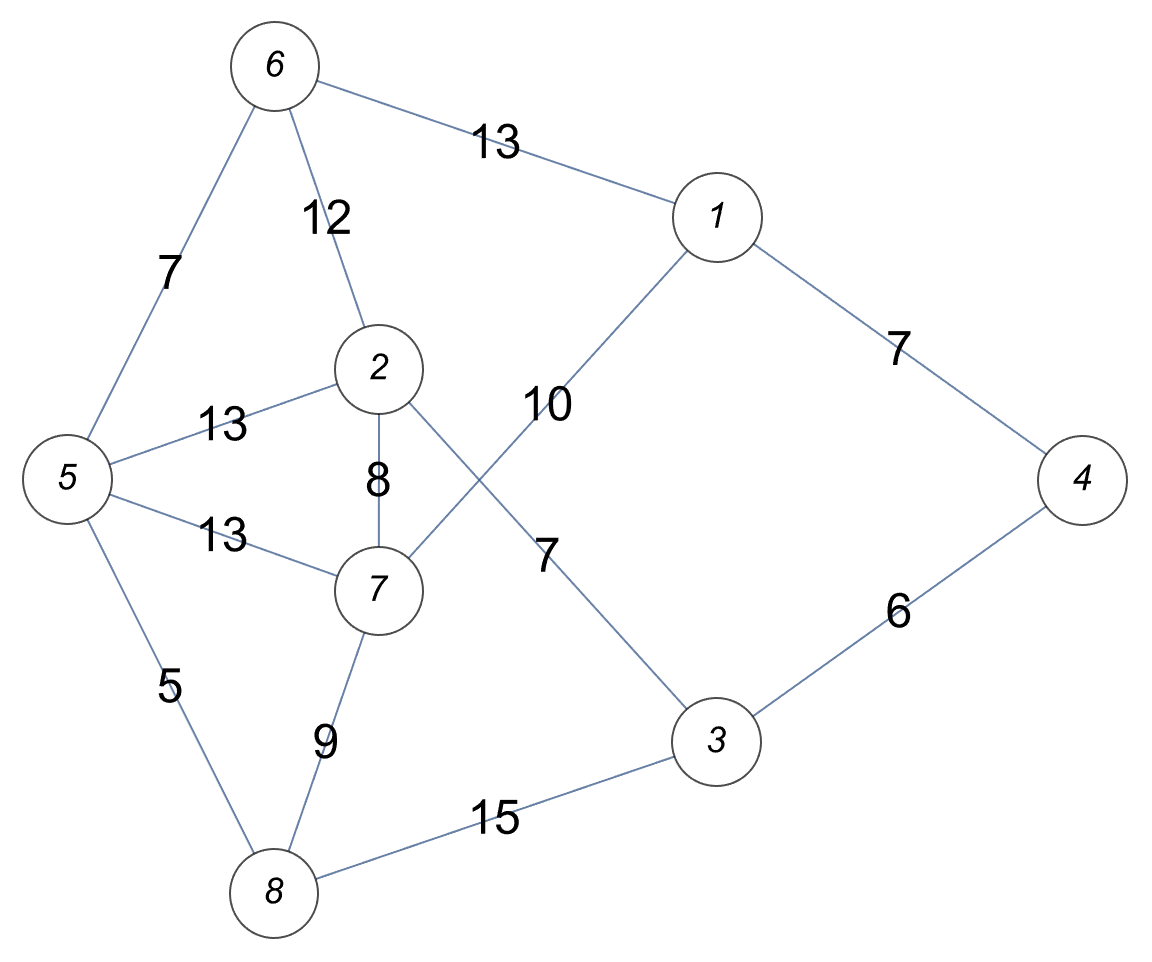
\includegraphics[width=\linewidth]{images/fig-prim-1.png}
\end{image}%
\tcblower
\end{figureptx}%
\par\smallskip%
\noindent\textbf{\blocktitlefont Solution}.\hypertarget{g:solution:idm218169879808}{}\quad{}The edges that are added, in order are \textbraceleft{}1,5\textbraceright{}, \textbraceleft{}1,9\textbraceright{}, \textbraceleft{}1,2\textbraceright{},\textbraceleft{}9,7\textbraceright{}, \textbraceleft{}7,6\textbraceright{},\textbraceleft{}7,3\textbraceright{},\textbraceleft{}1,10\textbraceright{},\textbraceleft{}5,8\textbraceright{},\textbraceleft{}9,4\textbraceright{}.  This assumes that if there is a tie in possibly adding an edge, the smallest vertex number is added, which is the case when \textbraceleft{}1,2\textbraceright{} is added.%
\end{divisionexerciseeg}%
\begin{divisionexerciseeg}{5}{}{}{g:exercise:idm218169879312}%
For each degree sequence below, decide whether it must always, must never, or could possibly be a degree sequence for a tree.  If it is always a tree, is the tree unique?  Justify your answers. (Adapted from \hyperlink{x:biblio:biblio-levin-2020}{[{\xreffont 3}]}.)%
\begin{enumerate}[label=(\alph*)]
\item{}\(\displaystyle (3, 3, 2, 2, 2)\)%
\item{}\(\displaystyle (3, 2, 2, 1, 1, 1)\)%
\item{}\(\displaystyle (3, 3, 3, 1, 1, 1)\)%
\item{}\(\displaystyle (4, 4, 1, 1, 1, 1, 1, 1)\)%
\end{enumerate}
%
\end{divisionexerciseeg}%
\end{exercisegroup}
\par\medskip\noindent
\end{exercises-subsection-numberless}
\end{sectionptx}
%
%
\typeout{************************************************}
\typeout{Section 30.3 Euler's Formula}
\typeout{************************************************}
%
\begin{sectionptx}{Euler's Formula}{}{Euler's Formula}{}{}{x:section:handouts-105}
\begin{theorem}{Euler's Formula.}{}{x:theorem:theorem-euler-formula-statement}%
\index{Euler's Formula}%
If \(G = (V, E)\) is a connected planar graph with \(r\) regions, \(v\) vertices, and \(e\) edges, then%
\begin{equation*}
v + r - e = 2
\end{equation*}
%
\end{theorem}
\end{sectionptx}
\end{chapterptx}
 %
%
\typeout{************************************************}
\typeout{Chapter 31 Rooted Trees, Binary Trees}
\typeout{************************************************}
%
\begin{chapterptx}{Rooted Trees, Binary Trees}{}{Rooted Trees, Binary Trees}{}{}{x:chapter:chapter_106}
\index{}%
%
%
\typeout{************************************************}
\typeout{Section 31.1 Reading Assignment}
\typeout{************************************************}
%
\begin{sectionptx}{Reading Assignment}{}{Reading Assignment}{}{}{x:section:reading-106}
Read Sections 10.3 and 10.4 of \emph{Applied Discrete Structures}. Here we consider some more structured trees in which a specific vertex is designated as the \emph{root} of the tree.  We see that there are several applications of these trees.  Special attention is given to binary trees, where no more than two edges branch away from the root and any away other vertex that is reached by the root.%
\begin{question}{Response Question.}{g:question:idm218169866560}%
The level of a vertex of a binary tree is the length of the path from the root to that vertex.  What is the maximum number of vertices at levels \(1, 2, 3, \dots\) of any binary tree?%
\end{question}
Also, turn in solutions to these exercises:%
%
%
\typeout{************************************************}
\typeout{Exercises 31.1 Exercises}
\typeout{************************************************}
%
\begin{exercises-subsection-numberless}{Exercises}{}{Exercises}{}{}{g:exercises:idm218169864640}
\par\medskip\noindent%
%
\begin{exercisegroup}
\begin{divisionexerciseeg}{1}{}{}{g:exercise:idm218169864384}%
Draw all different ordered rooted trees with four vertices.%
\end{divisionexerciseeg}%
\begin{divisionexerciseeg}{2}{}{}{g:exercise:idm218169863680}%
Construct the expression trees for the expressions \(\frac{a\cdot x + b}{c\cdot x + d}\) and and \(\frac{a}{c}+\frac{r}{c\cdot x + d}\).%
\end{divisionexerciseeg}%
\end{exercisegroup}
\par\medskip\noindent
\end{exercises-subsection-numberless}
\end{sectionptx}
%
%
\typeout{************************************************}
\typeout{Section 31.2 In-Class Exercises}
\typeout{************************************************}
%
\begin{sectionptx}{In-Class Exercises}{}{In-Class Exercises}{}{}{x:section:questions-106}
%
%
%
\typeout{************************************************}
\typeout{Exercises 31.2 Exercises}
\typeout{************************************************}
%
\begin{exercises-subsection-numberless}{Exercises}{}{Exercises}{}{}{g:exercises:idm218169861472}
\par\medskip\noindent%
%
\begin{exercisegroup}
\begin{divisionexerciseeg}{1}{}{}{g:exercise:idm218169861216}%
Given the list of data \mono{[483,569,150,649,659,198,356,241,359,930]}, insert the data sequentially into a binary sorting tree.%
\end{divisionexerciseeg}%
\begin{divisionexerciseeg}{2}{}{}{g:exercise:idm218169859920}%
List the vertices in a postorder traversal of the  expression tree of \(\frac{a x + b}{c x + d}\).%
\end{divisionexerciseeg}%
\begin{divisionexerciseeg}{3}{}{}{g:exercise:idm218169858864}%
Suppose \(0 \lt k \lt n\). Define the \(\binom{n}{k}\)-tree to be the binary tree with \(\binom{n}{k}\) at its root and left and right subtrees having roots \(\binom{n-1}{k-1}\) and \(\binom{n-1}{k}\), respectively. If \(k=0\) or \(k=n\), then the \(\binom{n}{k}\)-tree is a leaf containing the number 1.%
\begin{enumerate}[label=(\alph*)]
\item{}Draw the \(\binom{5}{1}\) and \(\binom{5}{2}\) trees.%
\item{}How many leaves does a \(\binom{n}{k}\)-tree contain?  Prove your answer.%
\end{enumerate}
%
\end{divisionexerciseeg}%
\begin{divisionexerciseeg}{4}{}{}{g:exercise:idm218169858480}%
How many binary trees are there having \(n\) vertices and an empty right subtree?%
\par\smallskip%
\noindent\textbf{\blocktitlefont Hint}.\hypertarget{g:hint:idm218169851152}{}\quad{}Use the formula for the number of binary trees with \(n\) vertices.%
\par\smallskip%
\noindent\textbf{\blocktitlefont Answer}.\hypertarget{g:answer:idm218169850224}{}\quad{}\(\frac{1}{n} \binom{2(n-1)}{n-1}\)%
\end{divisionexerciseeg}%
\begin{divisionexerciseeg}{5}{}{}{g:exercise:idm218169850640}%
\begin{sidebyside}{2}{0}{0}{0}%
\begin{sbspanel}{0.5}%
There is a one to one correspondence between ordered rooted trees and binary trees.  If you start with an ordered rooted tree, \(T\), you can build a binary tree \(B\) with an empty right subtree by placing the the root of \(T\) at the root of \(B\).  Then for every vertex \(v\) from \(T\) that has been placed in \(B\), place it's leftmost child (if there is one) as \(v\)'s left child in \(B\). Make \(v\)'s next sibling (if there is one) in \(T\) the right child in \(B\).%
\end{sbspanel}%
\begin{sbspanel}{0.5}%
\begin{figureptx}{An ordered rooted tree with root \(r\).}{x:figure:fig-ex-ordered-tree}{}%
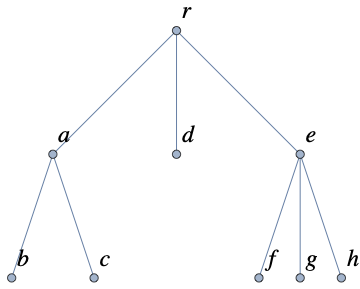
\includegraphics[width=\linewidth]{images/fig-ex-ordered-tree.png}
\tcblower
\end{figureptx}%
\end{sbspanel}%
\end{sidebyside}%
\begin{sidebyside}{2}{0}{0}{0}%
\begin{sbspanel}{0.5}%
\begin{figureptx}{Blue (left) and Red (right) links added to the ordered rooted tree with root r.}{x:figure:fig-ex-ordered-tree-linked}{}%
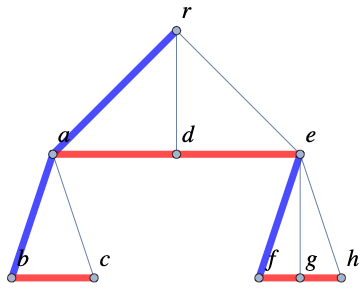
\includegraphics[width=\linewidth]{images/fig-ex-ordered-tree-linked.png}
\tcblower
\end{figureptx}%
\end{sbspanel}%
\begin{sbspanel}{0.5}%
\begin{figureptx}{Binary tree corresponding to the ordered rooted tree.}{x:figure:fig-ex-binary-tree}{}%
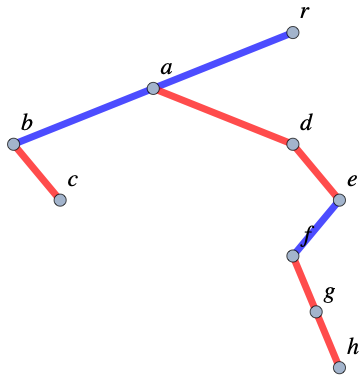
\includegraphics[width=\linewidth]{images/fig-ex-binary-tree.png}
\tcblower
\end{figureptx}%
\end{sbspanel}%
\end{sidebyside}%
\par
%
\begin{enumerate}[label=(\alph*)]
\item{}Why will \(B\) have no right children in this correspondence?%
\item{}Draw the binary tree that is produced by the ordered rooted tree in \hyperref[x:figure:fig-ort-to-bt]{Figure~{\xreffont\ref{x:figure:fig-ort-to-bt}}}.%
\item{}Draw the ordered tree that produces the binary tree in \hyperref[x:figure:fig-bt-to-ort]{Figure~{\xreffont\ref{x:figure:fig-bt-to-ort}}}.%
\item{}The left subtree of the binary tree in \hyperref[x:figure:fig-bt-to-ort]{Figure~{\xreffont\ref{x:figure:fig-bt-to-ort}}} is one of 5 different binary trees with three vertices.  Draw each of them and also the ordered rooted tree that each corresponds with.%
\item{}What does this correspondence tell us about how the numbers of different binary trees and ordered rooted trees are related?%
\end{enumerate}
%
\begin{sidebyside}{2}{0}{0}{0}%
\begin{sbspanel}{0.5}%
\begin{figureptx}{What binary tree does this correspond with?}{x:figure:fig-ort-to-bt}{}%
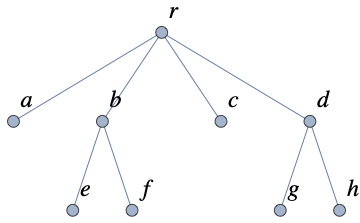
\includegraphics[width=\linewidth]{images/fig-ort-to-bt.png}
\tcblower
\end{figureptx}%
\end{sbspanel}%
\begin{sbspanel}{0.5}%
\begin{figureptx}{What ordered rooted tree does this correspond with?}{x:figure:fig-bt-to-ort}{}%
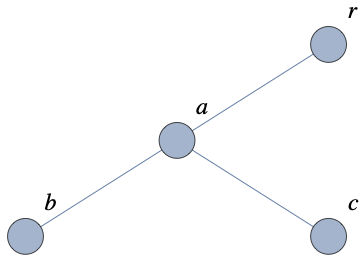
\includegraphics[width=\linewidth]{images/fig-bt-to-ort.png}
\tcblower
\end{figureptx}%
\end{sbspanel}%
\end{sidebyside}%
\par\smallskip%
\noindent\textbf{\blocktitlefont Solution}.\hypertarget{g:solution:idm218169829808}{}\quad{}%
\begin{enumerate}[label=(\alph*)]
\item{}The root of \(B\) is the root of the corresponding ordered rooted tree, which as no siblings.%
\item{}\begin{figureptx}{}{x:figure:fig-ort-to-bt_sol}{}%
\begin{image}{0.3}{0.4}{0.3}%
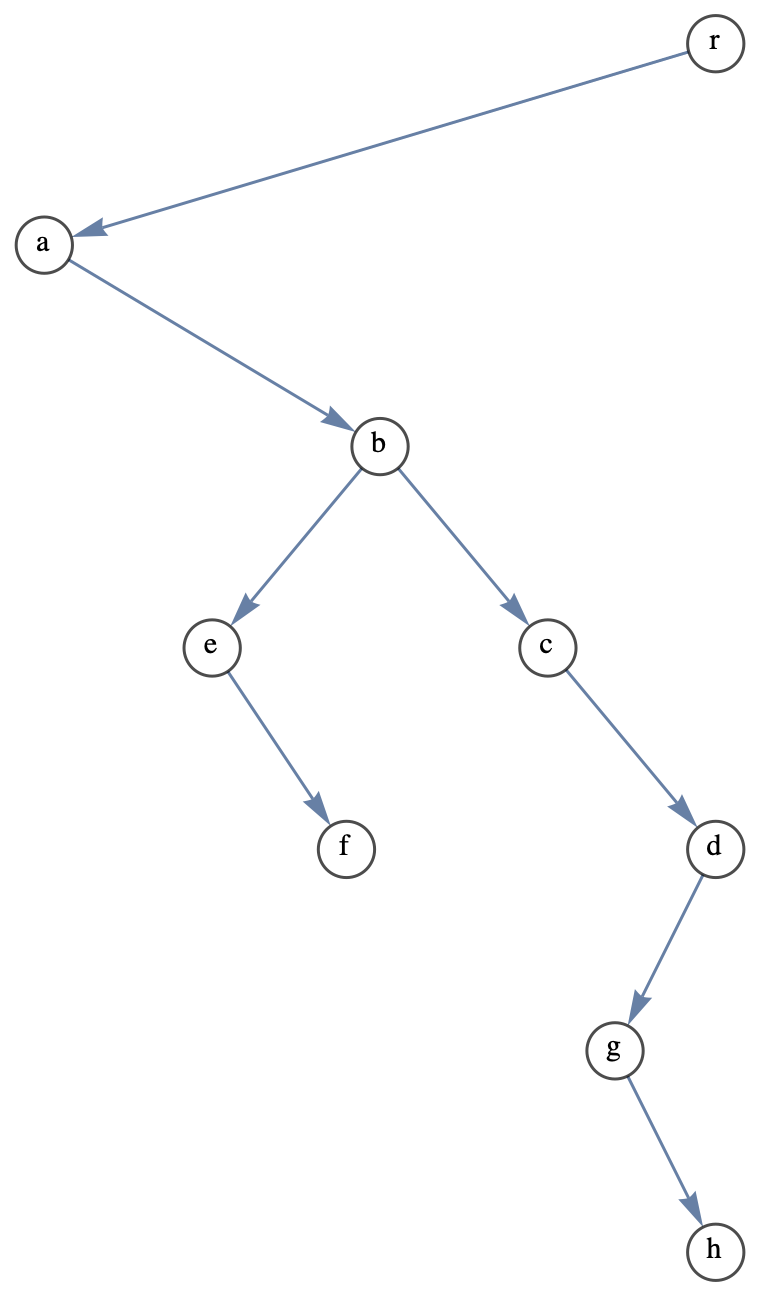
\includegraphics[width=\linewidth]{images/fig-ort-to-bt_sol.png}
\end{image}%
\tcblower
\end{figureptx}%
%
\item{}See below%
\item{}\begin{figureptx}{}{x:figure:fig-tree_correspondence}{}%
\begin{image}{0.15}{0.7}{0.15}%
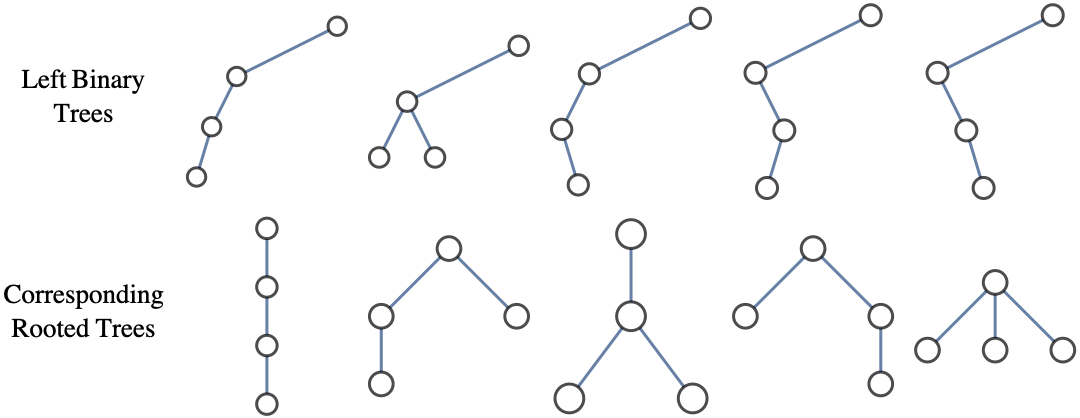
\includegraphics[width=\linewidth]{images/fig-tree_correspondence.png}
\end{image}%
\tcblower
\end{figureptx}%
%
\item{}The number of ordered rooted trees with \(n\) vertices is equal to the number of binary trees with \(n-1\) vertices, \(\frac{1}{n} \binom{2(n-1)}{n-1}\)%
\end{enumerate}
%
\end{divisionexerciseeg}%
\end{exercisegroup}
\par\medskip\noindent
\end{exercises-subsection-numberless}
\end{sectionptx}
\end{chapterptx}
 %
%
\typeout{************************************************}
\typeout{Chapter 32 Binary Operations}
\typeout{************************************************}
%
\begin{chapterptx}{Binary Operations}{}{Binary Operations}{}{}{x:chapter:chapter_107}
\index{}%
%
%
\typeout{************************************************}
\typeout{Section 32.1 Reading Assignment}
\typeout{************************************************}
%
\begin{sectionptx}{Reading Assignment}{}{Reading Assignment}{}{}{x:section:reading-107}
Read Section 11.1 of \emph{Applied Discrete Structures}. This is the beginning of a new topic, but you'll find that there are connections between algebra and graph theory.   In this first section we review properties of binary operations.%
\begin{question}{Response Question.}{g:question:idm218169802704}%
True or False?  Multiplication is an associative operation on the set \(\{-1,1\}\).  Justify your answer.%
\end{question}
Also, turn in solutions to these exercises:%
%
%
\typeout{************************************************}
\typeout{Exercises 32.1 Exercises}
\typeout{************************************************}
%
\begin{exercises-subsection-numberless}{Exercises}{}{Exercises}{}{}{g:exercises:idm218169801296}
\par\medskip\noindent%
%
\begin{exercisegroup}
\begin{divisionexerciseeg}{1}{}{}{g:exercise:idm218169801040}%
Explain why subtraction is not an associative operation on the integers.%
\par\smallskip%
\noindent\textbf{\blocktitlefont Solution}.\hypertarget{g:solution:idm218169800432}{}\quad{}A counterexample to the associative property is all that is needed here, of which there are an infinite number of examples.  One such is \(1-(2-3)\neq (1-2)-3\).%
\end{divisionexerciseeg}%
\begin{divisionexerciseeg}{2}{}{}{g:exercise:idm218169799344}%
Write out the operation table for intersection on the \(\mathcal{P}(\{0,1\})\), the power set of \(\{0,1\}\).%
\par\smallskip%
\noindent\textbf{\blocktitlefont Solution}.\hypertarget{g:solution:idm218169797952}{}\quad{}%
\end{divisionexerciseeg}%
\end{exercisegroup}
\par\medskip\noindent
\end{exercises-subsection-numberless}
\end{sectionptx}
%
%
\typeout{************************************************}
\typeout{Section 32.2 In-Class Exercises}
\typeout{************************************************}
%
\begin{sectionptx}{In-Class Exercises}{}{In-Class Exercises}{}{}{x:section:questions-107}
%
%
%
\typeout{************************************************}
\typeout{Exercises 32.2 Exercises}
\typeout{************************************************}
%
\begin{exercises-subsection-numberless}{Exercises}{}{Exercises}{}{}{g:exercises:idm218169796960}
\par\medskip\noindent%
%
\begin{exercisegroup}
\begin{divisionexerciseeg}{1}{}{}{g:exercise:idm218169796704}%
What properties that are introduced in Secton 11.1 are true of intersection on the power set of \(\{0,1\}\)?.%
\par\smallskip%
\noindent\textbf{\blocktitlefont Solution}.\hypertarget{g:solution:idm218169795456}{}\quad{}%
\end{divisionexerciseeg}%
\begin{divisionexerciseeg}{2}{}{}{g:exercise:idm218169795200}%
Consider the  operation \(\square\) on the  integers defined by%
\begin{equation*}
a \square b  = a+b-1.
\end{equation*}
%
\begin{enumerate}[label=(\alph*)]
\item{}Is \(\square\) associative?%
\item{}Does  \(\square\) have an identity in the positive integers?%
\item{}Does  \(\square\) have the inverse property?%
\end{enumerate}
%
\par\smallskip%
\noindent\textbf{\blocktitlefont Solution}.\hypertarget{g:solution:idm218169790656}{}\quad{}%
\begin{enumerate}[label=(\alph*)]
\item{}Yes, it is associative:%
\begin{gather*}
(a \square b)\square c= (a+b-1)\square c = a+b-1+c-1 = a+b+c-2\\
a \square(b \square c)= a \square(b+c-1) = a+(b+c-1)-1 = a+b+c-2
\end{gather*}
%
\item{}If \(e\) is an identity,  we would need \(a \square e=a+e-1 = a.\)  Solving \(a+e-1 = a\) for \(e\), we see that 1 is an identity.%
\item{}No, the inverse of a postitive integer \(a\)  would be \(b\)   such that \(a \square b=1\).   Therefore \(a+b-1=1\), or \(b=-a+2\).  But since we assume \(a\) is a positive integer \(b\) is not positive unless \(a = 1\),  and so only 1 have an inverse.%
\end{enumerate}
%
\end{divisionexerciseeg}%
\begin{divisionexerciseeg}{3}{}{}{g:exercise:idm218169786304}%
This question is open-ended, with no specific ``right'' answer.  Suppose that \(V\) is some finite nonempty set. What would be an example of a binary operation on the set of all undirected graphs with vertex set\(V\)?%
\par\smallskip%
\noindent\textbf{\blocktitlefont Solution}.\hypertarget{g:solution:idm218169780944}{}\quad{}%
\end{divisionexerciseeg}%
\end{exercisegroup}
\par\medskip\noindent
\end{exercises-subsection-numberless}
\end{sectionptx}
\end{chapterptx}
 %
%
\typeout{************************************************}
\typeout{Chapter 33 Algebraic Structures}
\typeout{************************************************}
%
\begin{chapterptx}{Algebraic Structures}{}{Algebraic Structures}{}{}{x:chapter:chapter_108}
\index{}%
%
%
\typeout{************************************************}
\typeout{Section 33.1 Reading Assignment}
\typeout{************************************************}
%
\begin{sectionptx}{Reading Assignment}{}{Reading Assignment}{}{}{x:section:reading-108}
Read Section 10.2 of \emph{Applied Discrete Structures}. We start by introducing the idea of levels of abstraction as they apply to monoids.  We then introduce groups, which is the main type of system we focus on in this chapter.%
\begin{question}{Response Question.}{g:question:idm218169778160}%
Discuss the connection between groups and monoids. Is every monoid a group? Is every group a monoid?%
\end{question}
Also, turn in solutions to these exercises:%
%
%
\typeout{************************************************}
\typeout{Exercises 33.1 Exercises}
\typeout{************************************************}
%
\begin{exercises-subsection-numberless}{Exercises}{}{Exercises}{}{}{g:exercises:idm218169776944}
\par\medskip\noindent%
%
\begin{exercisegroup}
\begin{divisionexerciseeg}{1}{}{}{g:exercise:idm218169776688}%
Write out the operation table for multiplication on the set \(\{1,-1,i, -i\}\).%
\par\smallskip%
\noindent\textbf{\blocktitlefont Solution}.\hypertarget{g:solution:idm218169775440}{}\quad{}%
\end{divisionexerciseeg}%
\begin{divisionexerciseeg}{2}{}{}{g:exercise:idm218169775184}%
How many different commutative binary operations are there on any two element set?%
\par\smallskip%
\noindent\textbf{\blocktitlefont Solution}.\hypertarget{g:solution:idm218169775856}{}\quad{}%
\end{divisionexerciseeg}%
\end{exercisegroup}
\par\medskip\noindent
\end{exercises-subsection-numberless}
\end{sectionptx}
%
%
\typeout{************************************************}
\typeout{Section 33.2 In-Class Exercises}
\typeout{************************************************}
%
\begin{sectionptx}{In-Class Exercises}{}{In-Class Exercises}{}{}{x:section:questions-108}
%
%
%
\typeout{************************************************}
\typeout{Exercises 33.2 Exercises}
\typeout{************************************************}
%
\begin{exercises-subsection-numberless}{Exercises}{}{Exercises}{}{}{g:exercises:idm218169773808}
\par\medskip\noindent%
%
\begin{exercisegroup}
\begin{divisionexerciseeg}{1}{}{}{g:exercise:idm218169773472}%
Let \(U\) be a any set.  Prove that, \(\oplus\), defined by \(A \oplus  B = (A \cup  B) - (A \cap  B)\) is an associative operation on \(\mathcal{P}(U)\).%
\end{divisionexerciseeg}%
\begin{divisionexerciseeg}{2}{}{}{g:exercise:idm218169770832}%
Let \(U\) be a any set.  Prove that,   \([\mathcal{P}(U); \oplus]\) is a group.%
\end{divisionexerciseeg}%
\begin{divisionexerciseeg}{3}{}{}{g:exercise:idm218169771248}%
Consider the following set of six  algebraic expressions, each defining a function on the set of real numbers excluding the numbers 0 and 1.%
\begin{equation*}
\mathcal{H}=\left\{x,1-x,\frac{1}{1-x},\frac{1}{x},\frac{x-1}{x},\frac{x}{x-1}\right\}
=\left\{y_1,y_2,y_3,y_4,y_5,y_6\right\}
\end{equation*}
We can opperate on any two of these expressions using function composition.  For example,%
\begin{equation*}
(y_3 \circ y_4)(x) = y_3(y_4(x))=y_3(\frac{1}{x})=\frac{1}{1-\frac{1}{x}}=\frac{x}{x-1}=y_6(x)
\end{equation*}
Therefore, \(y_3 \circ y_4 = y_6\).  Complete the following operation table for function composition on \(\mathcal{H}\).%
\begin{figureptx}{Partially completed operation table for \(\mathcal{H}\)}{x:figure:fig-compositon_group_6}{}%
\begin{image}{0.15}{0.7}{0.15}%
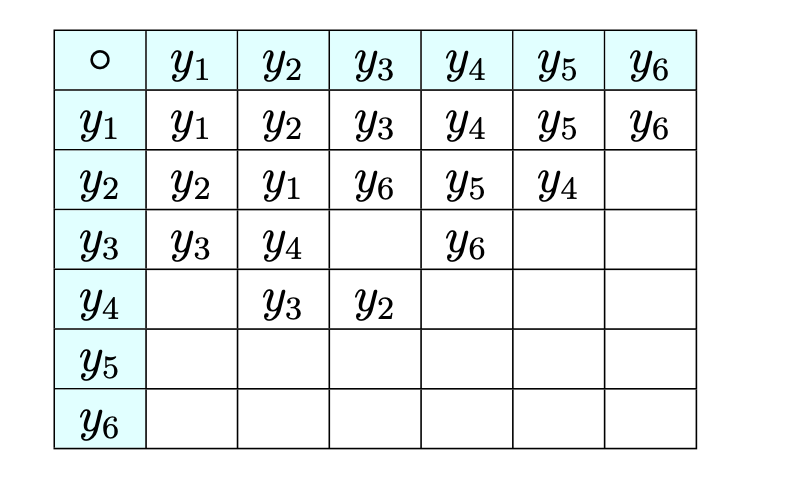
\includegraphics[width=\linewidth]{images/fig-compositon_group_6.png}
\end{image}%
\tcblower
\end{figureptx}%
Is \([\mathcal{H},\circ]\) a monoid? Is it a group?%
\par\smallskip%
\noindent\textbf{\blocktitlefont Solution}.\hypertarget{g:solution:idm218169763168}{}\quad{}%
\end{divisionexerciseeg}%
\begin{divisionexerciseeg}{4}{}{}{g:exercise:idm218169762816}%
Let \(S\) be the set of all strings of letters of length zero or more from the set \(\{a,b,c\}\) that do not have any consecutive identical letters.  Define \(*\) on \(S\) by the rule that if \(x, y \in S\) then \(x*y\) is determined by first concatenating  \(x\) and \(y\) and then repeatedly removing any occurrences of two identical letters until the result is an element of \(S\).   Is \([S,*]\) a monoid?  Is it a group?%
\par\smallskip%
\noindent\textbf{\blocktitlefont Solution}.\hypertarget{g:solution:idm218169762432}{}\quad{}%
\end{divisionexerciseeg}%
\end{exercisegroup}
\par\medskip\noindent
\end{exercises-subsection-numberless}
\end{sectionptx}
\end{chapterptx}
 %
%
\typeout{************************************************}
\typeout{Chapter 34 Properties of Groups}
\typeout{************************************************}
%
\begin{chapterptx}{Properties of Groups}{}{Properties of Groups}{}{}{x:chapter:chapter_109}
\index{group!properties}%
%
%
\typeout{************************************************}
\typeout{Section 34.1 Reading Assignment}
\typeout{************************************************}
%
\begin{sectionptx}{Reading Assignment}{}{Reading Assignment}{}{}{x:section:reading-109}
Read Section 11.3 of \emph{Applied Discrete Structures}.  In this section we examine some of the basic theorems that follow immediately from the axioms of a group. Reviewing the proofs is a good exercise in solidifying an understanding of the axioms. In most cases, these theorems are applied in later work without explicitly stating them.%
\begin{question}{Response Question.}{g:question:idm218169754496}%
SageMath can be used to explore concrete groups.  It can't be used to prove significant theorems, but you can verify that the theorems are true.  Here is one particular group's operation table generated using Sage. The group, with domain \mono{[a,b,c,d,e,f,g,h]}, is in a family called the dihedral groups, and will be encountered in Section 15.3. For the purposes of this question, notice that in the body of the table, each element appears exactly once in each row and column.  Which theorem guarantees that this is always true for a group's operation table?%
\begin{sageinput}
G=DihedralGroup(4)
G.cayley_table()
\end{sageinput}
\begin{sageoutput}
*  a b c d e f g h
 +----------------
a| a b c d e f g h
b| b a d c f e h g
c| c g a e d h b f
d| d h b f c g a e
e| e f g h a b c d
f| f e h g b a d c
g| g c e a h d f b
h| h d f b g c e a
\end{sageoutput}
\par\smallskip%
\noindent\textbf{\blocktitlefont Answer}.\hypertarget{g:answer:idm218169751632}{}\quad{}Any of of the following theorems could be applied to make this observation: Cancellation Laws, Linear Equations in a Groups, or the Pigeonhole Principle.%
\end{question}
Also, do these exercises:%
%
%
\typeout{************************************************}
\typeout{Exercises 34.1 Exercises}
\typeout{************************************************}
%
\begin{exercises-subsection-numberless}{Exercises}{}{Exercises}{}{}{g:exercises:idm218169750832}
\par\medskip\noindent%
%
\begin{exercisegroup}
\begin{divisionexerciseeg}{1}{}{}{g:exercise:idm218169750576}%
Suppose \([G;*]\) is a group with \(a,b,c \in G\).   Solve the equation%
\begin{equation*}
a*x*a^{-1}*b= c
\end{equation*}
for \(x\).%
\par\smallskip%
\noindent\textbf{\blocktitlefont Solution}.\hypertarget{g:solution:idm218169748128}{}\quad{}%
\end{divisionexerciseeg}%
\begin{divisionexerciseeg}{2}{}{}{g:exercise:idm218169747872}%
Notice that \(\{1,2,3\} \cap \{1,2\} = \{1,2,3,4\} \cap \{1,2\}\), yet \(\{1,2,3\}  \neq \{1,2,3,4\} \). Does this contradict the \hyperref[x:theorem:theorem-11-3-cancellation]{Cancellation Laws}? Explain your answer.%
\par\smallskip%
\noindent\textbf{\blocktitlefont Solution}.\hypertarget{g:solution:idm218169745744}{}\quad{}A%
\end{divisionexerciseeg}%
\end{exercisegroup}
\par\medskip\noindent
\end{exercises-subsection-numberless}
\end{sectionptx}
%
%
\typeout{************************************************}
\typeout{Section 34.2 In-Class Exercises}
\typeout{************************************************}
%
\begin{sectionptx}{In-Class Exercises}{}{In-Class Exercises}{}{}{x:section:questions-109}
%
%
%
\typeout{************************************************}
\typeout{Exercises 34.2 Exercises}
\typeout{************************************************}
%
\begin{exercises-subsection-numberless}{Exercises}{}{Exercises}{}{}{g:exercises:idm218169744528}
\par\medskip\noindent%
%
\begin{exercisegroup}
\begin{divisionexerciseeg}{1}{}{}{g:exercise:idm218169744272}%
Prove that if \(a^2 = e\) for all elements \(a\) in a group \(G\), then \(G\) must be abelian.%
\par\smallskip%
\noindent\textbf{\blocktitlefont Hint}.\hypertarget{g:hint:idm218169741904}{}\quad{}Given \(a, b \in G\), apply the premise to \(a*b\).%
\end{divisionexerciseeg}%
\begin{divisionexerciseeg}{2}{}{}{g:exercise:idm218169740672}%
Suppose \([G;*]\) is a group and \(a \in G\).  Define \(f_a:G \to  G\) by \(f_a(x) = a * x\).  If we compose two such functions, \(f_a\) and \(f_b\) where \(a, b \in G\), what function do we get for \(f_a \circ f_b\)?%
\par\smallskip%
\noindent\textbf{\blocktitlefont Solution}.\hypertarget{g:solution:idm218169740288}{}\quad{}%
\end{divisionexerciseeg}%
\begin{divisionexerciseeg}{3}{}{}{g:exercise:idm218169736560}%
This problem anticipates a future topic that you can plausibly discover on your own. Functions like the ones in the previous problem can be of use in this one.%
\par
Suppose \([G;*]\) is a finite group of order \(n\). The \hyperref[x:theorem:theorem-11-3-finite]{last theorem in Section 11.3} in Section 10.3 states that if \(a\in G\), there exists a positive integer, \(m\) less than \(n\) such that \(a^m=e\).  Prove that the least such positive integer is a divisor of \(n\).%
\par\smallskip%
\noindent\textbf{\blocktitlefont Hint}.\hypertarget{g:hint:idm218169735760}{}\quad{}You can partition \(G\) into subsets of equal cardinality.%
\par\smallskip%
\noindent\textbf{\blocktitlefont Solution}.\hypertarget{g:solution:idm218169730864}{}\quad{}Let \(H\) be the set of distinct powers of \(a\).  This is a finite set since it's a subset of a finite set.  Pick any element \(a\) of \(G\) that's not in \(H\).  The function \(f_a:H \rightarrow G\) from the last problem of the week is a one-to-one function (this implied by the cancellation laws).  The range of \(f_a\),  \(f_a(H)\), has the same cardinality as \(H\).  Keep repeating the process, at each stage selecting an element of \(G\) that's not appeared in \(H\) or any of the ranges of functions from previous steps.   This process has to end in a finite number of steps and produces a partition of \(G\) into subsets all of the same cardinality as \(H\).%
\end{divisionexerciseeg}%
\end{exercisegroup}
\par\medskip\noindent
\end{exercises-subsection-numberless}
\end{sectionptx}
%
%
\typeout{************************************************}
\typeout{Section 34.3 Some Theorems}
\typeout{************************************************}
%
\begin{sectionptx}{Some Theorems}{}{Some Theorems}{}{}{x:section:handouts-109}
Two of the theorems in Section 10.3 follow. In doing the exercises, you don't need to prove these theorems or the others in the section.%
\begin{theorem}{Cancellation Laws.}{}{x:theorem:theorem-11-3-cancellation}%
\index{Cancellation in Groups}%
If \(a\), \(b\), and \(c\) are elements of group \(G\), then%
\begin{equation*}
\begin{array}{lc}
\textrm{left cancellation: }& (a * b = a * c)  \Rightarrow b = c\\
\textrm{right cancellation: }&  (b * a = c * a) \Rightarrow b = c\\
\end{array}
\end{equation*}
%
\end{theorem}
\begin{theorem}{last theorem in Section 11.3.}{}{x:theorem:theorem-11-3-finite}%
If \(G\) is a finite group,  \(\left| G\right| = n\), and \(a\) is an element of \(G\), then there exists a positive integer \(m\) such that \(a^m= e\) and \(m\leq n\).%
\end{theorem}
\end{sectionptx}
\end{chapterptx}
 %
%
\typeout{************************************************}
\typeout{Chapter 35 Modular Arithmetic}
\typeout{************************************************}
%
\begin{chapterptx}{Modular Arithmetic}{}{Modular Arithmetic}{}{}{x:chapter:chapter_110}
\index{Modular Arithmetic}%
%
%
\typeout{************************************************}
\typeout{Section 35.1 Reading Assignment}
\typeout{************************************************}
%
\begin{sectionptx}{Reading Assignment}{}{Reading Assignment}{}{}{x:section:reading-110}
Read Section 11.4 of \emph{Applied Discrete Structures}. The definitions of modular addition and multiplication in this section are \emph{really important}.  They are used throughout the rest of the book.  The section starts with a review of division properties for integers in order to set up the modular operations.  Generally, the mod \(n\) operations are operations only on either \(\mathbb{Z}_n\), or a subset of \(\mathbb{Z}_n\).  For example, it wouldn't make sense to do mod 10 addition on \(Z_{12}\).%
\begin{question}{Response Question.}{g:question:idm218169714016}%
If the product of two numbers is zero, must one of the numbers equal zero?%
\end{question}
Also, turn in solutions to the following exercises.  Both of them could be done using SageMath by typing two short inputs, but you are encouraged to write (or type) both of these be hand.%
%
%
\typeout{************************************************}
\typeout{Exercises 35.1 Exercises}
\typeout{************************************************}
%
\begin{exercises-subsection-numberless}{Exercises}{}{Exercises}{}{}{g:exercises:idm218169709520}
\par\medskip\noindent%
%
\begin{exercisegroup}
\begin{divisionexerciseeg}{1}{}{}{g:exercise:idm218169709184}%
Compute by hand the greatest common divisor of \(2028\)  and \(1001\).  Show the calculations you did to get your answer.%
\par\smallskip%
\noindent\textbf{\blocktitlefont Solution}.\hypertarget{g:solution:idm218169707632}{}\quad{}%
\end{divisionexerciseeg}%
\begin{divisionexerciseeg}{2}{}{}{g:exercise:idm218169707296}%
Write out the operation table for mod 4 addition on \(\mathbb{Z}_4\).  Identify the inverse of each element.%
\par\smallskip%
\noindent\textbf{\blocktitlefont Solution}.\hypertarget{g:solution:idm218169706160}{}\quad{}%
\end{divisionexerciseeg}%
\end{exercisegroup}
\par\medskip\noindent
\end{exercises-subsection-numberless}
\end{sectionptx}
%
%
\typeout{************************************************}
\typeout{Section 35.2 In-Class Exercises}
\typeout{************************************************}
%
\begin{sectionptx}{In-Class Exercises}{}{In-Class Exercises}{}{}{x:section:questions-110}
%
%
%
\typeout{************************************************}
\typeout{Exercises 35.2 Exercises}
\typeout{************************************************}
%
\begin{exercises-subsection-numberless}{Exercises}{}{Exercises}{}{}{g:exercises:idm218169705136}
\par\medskip\noindent%
%
\begin{exercisegroup}
\begin{divisionexerciseeg}{1}{}{}{g:exercise:idm218169704880}%
Let \(n\) be a positive integer greater than 1.  Show that \(n-1\) has a multiplicative inverse mod \(n\).%
\par\smallskip%
\noindent\textbf{\blocktitlefont Solution}.\hypertarget{g:solution:idm218169702816}{}\quad{}Since \(gcd(n,n-1)=gcd(n-1,1)=1\), \(n-1\) has a mod \(n\) inverse.  In fact, it is its own inverse.%
\end{divisionexerciseeg}%
\begin{divisionexerciseeg}{2}{}{}{g:exercise:idm218169701120}%
Compute by hand the additive and multiplicative inverses of 653 mod 1001. Show the calculations you did to get your answer.%
\par\smallskip%
\noindent\textbf{\blocktitlefont Solution}.\hypertarget{g:solution:idm218169700480}{}\quad{}%
\end{divisionexerciseeg}%
\begin{divisionexerciseeg}{3}{}{}{g:exercise:idm218169700224}%
Write out the operation table for the multiplicative group of integers mod 8  on \(\mathbb{U}_8= \{k \in \mathbb{Z}_8 \mid \gcd{(8,k)}=1\}\).  Identify the inverse of each element.%
\par\smallskip%
\noindent\textbf{\blocktitlefont Solution}.\hypertarget{g:solution:idm218169699152}{}\quad{}%
\end{divisionexerciseeg}%
\begin{divisionexerciseeg}{4}{}{}{g:exercise:idm218169699584}%
Write out the operation table for mod 10 multiplication on \(T=\{0,2,4,6,8\}\). Is \([T;\times_{10}]\)	 a monoid? Is it a group?%
\par\smallskip%
\noindent\textbf{\blocktitlefont Solution}.\hypertarget{g:solution:idm218169697536}{}\quad{}%
\end{divisionexerciseeg}%
\begin{divisionexerciseeg}{5}{}{}{g:exercise:idm218169697280}%
Find a formula for the inverse of the function \(g: \mathbb{Z}_{29} \rightarrow  \mathbb{Z}_{29}\) where \(g(a)= 5\times_{29}a +_{29}25\).  Suggestion:  You can use the symbols \(\times\) and \(+\) in your work instead of \(\times_{29}\) and \(+_{29}\) as long as we agree that they stand for mod 29 operations.%
\par\smallskip%
\noindent\textbf{\blocktitlefont Answer}.\hypertarget{g:answer:idm218169696896}{}\quad{}\(g^{-1}(a) = 6 \times_{29}(a +_{29} 4)\)%
\par\smallskip%
\noindent\textbf{\blocktitlefont Solution}.\hypertarget{g:solution:idm218169693344}{}\quad{}%
\end{divisionexerciseeg}%
\end{exercisegroup}
\par\medskip\noindent
\end{exercises-subsection-numberless}
\end{sectionptx}
\end{chapterptx}
 %
%
\typeout{************************************************}
\typeout{Chapter 36 Subsystems}
\typeout{************************************************}
%
\begin{chapterptx}{Subsystems}{}{Subsystems}{}{}{x:chapter:chapter_111}
\index{Subsystem}%
\index{Subgroup}%
\index{Cyclic Subgroup}%
%
%
\typeout{************************************************}
\typeout{Section 36.1 Reading Assignment}
\typeout{************************************************}
%
\begin{sectionptx}{Reading Assignment}{}{Reading Assignment}{}{}{x:section:reading-111}
Read Section 11.5 of \emph{Applied Discrete Structures}. The main idea is that there are certain subsets of groups that qualify as groups in their own right.  This is an instance of a more general situation in mathematics where a structure can contain smaller structures.  The idea of a subset is the most simple case of this, but we have also seen subgraphs in the study of graphs and trees.  Finding all subgroups of a group isn't always easy, but describing and finding the cyclic subgroups of a group is not too difficult.  Pay close attention how this is done!%
\begin{question}{Response Question.}{g:question:idm218169689600}%
Let \(m \mathbb{Z} = \{m \cdot k \mid k \in \mathbb{Z}\}\). Chris says that \(7 \mathbb{Z}\) is a subgroup of \(14 \mathbb{Z}\) because \(7 \leq 14\).   How would you respond to Chris?%
\end{question}
Also, turn in solutions to these exercises:%
%
%
\typeout{************************************************}
\typeout{Exercises 36.1 Exercises}
\typeout{************************************************}
%
\begin{exercises-subsection-numberless}{Exercises}{}{Exercises}{}{}{g:exercises:idm218169686640}
\par\medskip\noindent%
%
\begin{exercisegroup}
\begin{divisionexerciseeg}{1}{}{}{g:exercise:idm218169686384}%
True or false?:  The set of all bit strings that begin with a 1 form a submonoid of the monoid of all bit strings with concatination.%
\par\smallskip%
\noindent\textbf{\blocktitlefont Solution}.\hypertarget{g:solution:idm218169685488}{}\quad{}The statement is false because the empty string doesn't start with a 1 and so the identity element is not in the given set. Explain your answer.%
\end{divisionexerciseeg}%
\begin{divisionexerciseeg}{2}{}{}{g:exercise:idm218169684944}%
True or false?: \(\{0,25,50,75\}\) is a subgroup of the additive group \(\mathbb{Z}_{100}\). Explain your answer.%
\par\smallskip%
\noindent\textbf{\blocktitlefont Solution}.\hypertarget{g:solution:idm218169683488}{}\quad{}%
\end{divisionexerciseeg}%
\end{exercisegroup}
\par\medskip\noindent
\end{exercises-subsection-numberless}
\end{sectionptx}
%
%
\typeout{************************************************}
\typeout{Section 36.2 In-Class Exercises}
\typeout{************************************************}
%
\begin{sectionptx}{In-Class Exercises}{}{In-Class Exercises}{}{}{x:section:questions-111}
%
%
%
\typeout{************************************************}
\typeout{Exercises 36.2 Exercises}
\typeout{************************************************}
%
\begin{exercises-subsection-numberless}{Exercises}{}{Exercises}{}{}{g:exercises:idm218169682496}
\par\medskip\noindent%
%
\begin{exercisegroup}
\begin{divisionexerciseeg}{1}{}{}{g:exercise:idm218169682240}%
Determine the cyclic subgroup generated by 4 in the group \(\mathbb{Z}_{11}\)%
\par\smallskip%
\noindent\textbf{\blocktitlefont Solution}.\hypertarget{g:solution:idm218169681152}{}\quad{}%
\end{divisionexerciseeg}%
\begin{divisionexerciseeg}{2}{}{}{g:exercise:idm218169681440}%
Determine the cyclic subgroup generated by 4 in the group \(\mathbb{U}_{11}\)%
\par\smallskip%
\noindent\textbf{\blocktitlefont Solution}.\hypertarget{g:solution:idm218169680016}{}\quad{}%
\end{divisionexerciseeg}%
\begin{divisionexerciseeg}{3}{}{}{g:exercise:idm218169680304}%
In this exercise, we will consider the orders of the additive groups of integers modulo \(n\) for three different values of \(n\), and then speculate on some general results.%
\begin{enumerate}[label=(\alph*)]
\item{}Determine the orders of different elements of the group \(\mathbb{Z}_{5}\).%
\item{}Determine the orders of different elements of the group \(\mathbb{Z}_{15}\).%
\item{}Determine the orders of different elements of the group \(\mathbb{Z}_{16}\).%
\item{}Comparing the results you got above, hypothesize on what you would expect for different moduli%
\end{enumerate}
%
\par\smallskip%
\noindent\textbf{\blocktitlefont Solution}.\hypertarget{g:solution:idm218228546640}{}\quad{}%
\end{divisionexerciseeg}%
\begin{divisionexerciseeg}{4}{}{}{g:exercise:idm218228547536}%
Assume that \([G;*]\) is a group and \(H\) is a nonempty subset of \(G\). Suppose that we are told that for \(a, b \in H\), we are guaranteed that \(a^{-1}*b \in H\).  Prove that \(H\) is a subgroup of \(G\).%
\par\smallskip%
\noindent\textbf{\blocktitlefont Hint}.\hypertarget{g:hint:idm218228586240}{}\quad{}Prove the identity, inverses and closure properties of a subgroup, in that order.%
\par\smallskip%
\noindent\textbf{\blocktitlefont Solution}.\hypertarget{g:solution:idm218228587840}{}\quad{}%
\end{divisionexerciseeg}%
\end{exercisegroup}
\par\medskip\noindent
\end{exercises-subsection-numberless}
\end{sectionptx}
%
%
\typeout{************************************************}
\typeout{Section 36.3 Handouts}
\typeout{************************************************}
%
\begin{sectionptx}{Handouts}{}{Handouts}{}{}{x:section:handouts-111}
Here is a reminder of the definition of the associative property.%
\begin{definition}{Associative Property.}{x:definition:def-associative-property}%
\index{Associative Property}%
Let \(*\) be a binary operation on a set \(S\). We say that \(*\) is  \terminology{associative}  if and only if \((a * b) * c = a * (b * c)\) for all \(a, b, c \in  S\).%
\end{definition}
\end{sectionptx}
\end{chapterptx}
 %
%
\typeout{************************************************}
\typeout{Chapter 37 Direct Products}
\typeout{************************************************}
%
\begin{chapterptx}{Direct Products}{}{Direct Products}{}{}{x:chapter:chapter_112}
\index{Direct Products}%
%
%
\typeout{************************************************}
\typeout{Section 37.1 Reading Assignment}
\typeout{************************************************}
%
\begin{sectionptx}{Reading Assignment}{}{Reading Assignment}{}{}{x:section:reading-112}
Read Section 11.6 of \emph{Applied Discrete Structures}. At some point, you may have seen an ``addition'' of pairs that looked something like this:%
\begin{equation*}
(2,9)+(1,-3) = (2+1,9+(-3))=(3,6).
\end{equation*}
This is an example of ``coordinate-wise addition,'' where the first coordinate of the sum depends only on the two first coordinates of the terms on the left. This is exactly the way direct products work in general. In this section you will see what is produced from direct products of groups.%
\begin{question}{Response Question.}{g:question:idm218228662048}%
A fraction can be though of as an ordered pair, \(a/b\), where \(a\) is the numerator and nonzero \(b\) is the denominator.  Is addition of fractions a coordinate-wise operaton?%
\end{question}
Also, turn in solutions to this exercise:%
%
%
\typeout{************************************************}
\typeout{Exercises 37.1 Exercises}
\typeout{************************************************}
%
\begin{exercises-subsection-numberless}{Exercises}{}{Exercises}{}{}{g:exercises:idm218228672304}
\par\medskip\noindent%
%
\begin{exercisegroup}
\begin{divisionexerciseeg}{1}{}{}{g:exercise:idm218228673280}%
Write out the operation table for the group \(\mathbb{Z}_2 \times \mathbb{Z}_2\)%
\par\smallskip%
\noindent\textbf{\blocktitlefont Solution}.\hypertarget{g:solution:idm218228677520}{}\quad{}%
\end{divisionexerciseeg}%
\begin{divisionexerciseeg}{2}{}{}{g:exercise:idm218228700944}%
Find all elements of the cyclic subgroup generated by \((1,1)\) in the group \(\mathbb{Z}_2 \times \mathbb{Z}_3\).%
\par\smallskip%
\noindent\textbf{\blocktitlefont Solution}.\hypertarget{g:solution:idm218228730816}{}\quad{}%
\end{divisionexerciseeg}%
\end{exercisegroup}
\par\medskip\noindent
\end{exercises-subsection-numberless}
\end{sectionptx}
%
%
\typeout{************************************************}
\typeout{Section 37.2 In-Class Exercises}
\typeout{************************************************}
%
\begin{sectionptx}{In-Class Exercises}{}{In-Class Exercises}{}{}{x:section:questions-112}
%
%
%
\typeout{************************************************}
\typeout{Exercises 37.2 Exercises}
\typeout{************************************************}
%
\begin{exercises-subsection-numberless}{Exercises}{}{Exercises}{}{}{g:exercises:idm218228761440}
\par\medskip\noindent%
%
\begin{exercisegroup}
\begin{divisionexerciseeg}{1}{}{}{g:exercise:idm218228763984}%
Determine the following values in the group \(\mathbb{Z}_3 \times  \mathbb{R}^*\).  First, make sure you know what operations are involved in the two ``factors'' of this direct product.%
\begin{enumerate}[label=(\alph*)]
\item{}\(\displaystyle (2,1)* (1,2)\)%
\item{}the identity element%
\item{}\(\displaystyle (1, 1/2)^{-1}\)%
\end{enumerate}
%
\end{divisionexerciseeg}%
\begin{divisionexerciseeg}{2}{}{}{g:exercise:idm218228784608}%
Describe the elements of the cyclic subgroup generated by \((1,-1)\) in the group \(\mathbb{Z}^2\) as simply as possible.%
\par\smallskip%
\noindent\textbf{\blocktitlefont Answer}.\hypertarget{g:answer:idm218228797888}{}\quad{}\(\{(n,-n)\mid n \in \mathbb{Z}\}\)%
\end{divisionexerciseeg}%
\begin{divisionexerciseeg}{3}{}{}{g:exercise:idm218228801488}%
In the text, it was observed that if \(a, b \in  \mathbb{R}\),  then \(\{(x, y) \mid a x + b y = 0\}\) is subgroup of \(\mathbb{R}^2\).  Prove that this is true, and show that the similar set  \(\{(x, y) \mid a x + b y = c\}\) is not a subgroup when \(c \neq 0\).%
\par\smallskip%
\noindent\textbf{\blocktitlefont Solution}.\hypertarget{g:solution:idm218228826304}{}\quad{}%
\end{divisionexerciseeg}%
\begin{divisionexerciseeg}{4}{}{}{g:exercise:idm218228828192}%
A symmetric linked list in a five bit computer contains four nodes with the machine address of first node being \(11011\).  The link fields for the nodes in the list from first to last are \(00111, 00111, 10111, 11100\). Assume the nil pointer value is 00000.  What are the machine addresses of the nodes 2, 3 and 4?%
\par\smallskip%
\noindent\textbf{\blocktitlefont Answer}.\hypertarget{g:answer:idm218228850960}{}\quad{}The addresses of nodes 2 through 4 are \(00111, 11100, 10000\).%
\end{divisionexerciseeg}%
\end{exercisegroup}
\par\medskip\noindent
\end{exercises-subsection-numberless}
\end{sectionptx}
\end{chapterptx}
 %
%
\typeout{************************************************}
\typeout{Chapter 38 Isomorphisms}
\typeout{************************************************}
%
\begin{chapterptx}{Isomorphisms}{}{Isomorphisms}{}{}{x:chapter:chapter_113}
\index{Isomorphism}%
%
%
\typeout{************************************************}
\typeout{Section 38.1 Reading Assignment}
\typeout{************************************************}
%
\begin{sectionptx}{Reading Assignment}{}{Reading Assignment}{}{}{x:section:reading-113}
Read Section 11.7  of \emph{Applied Discrete Structures}.  We've seen several different groups of order two. Two of them are the group \(\mathbb{Z}_2\) and \([\{1,-1\}; \cdot]\).  There is no denying that these groups are different but from an algebraic point of view, they have all the same properties.   This section makes this observation more precise.  Based on the definitions, these two groups (and all other groups with two elements) are \emph{isomorphic}.  In studying groups, this is essentially saying they are all equal.%
\begin{question}{Response Question.}{g:question:idm218228885056}%
How is the topic of isomorphisms related to the \hyperref[x:figure:fig-slide-rule]{Slide Rule}, an analog computing device that was in common usage up until the 1970's.%
\end{question}
Also, turn in solutions to this exercise:%
%
%
\typeout{************************************************}
\typeout{Exercises 38.1 Exercises}
\typeout{************************************************}
%
\begin{exercises-subsection-numberless}{Exercises}{}{Exercises}{}{}{g:exercises:idm218228897904}
\par\medskip\noindent%
%
\begin{exercisegroup}
\begin{divisionexerciseeg}{1}{}{}{g:exercise:idm218228899328}%
Answer the following question:  siedem razy cztery = \textunderscore{}\textunderscore{}\textunderscore{}\textunderscore{}\textunderscore{}?%
\par\smallskip%
\noindent\textbf{\blocktitlefont Hint}.\hypertarget{g:hint:idm218228905280}{}\quad{}The question is in Polish.%
\par\smallskip%
\noindent\textbf{\blocktitlefont Solution}.\hypertarget{g:solution:idm218228910368}{}\quad{}%
\end{divisionexerciseeg}%
\begin{divisionexerciseeg}{2}{}{}{g:exercise:idm218228912432}%
The two groups \(\mathbb{Z}_4\) and \(\mathbb{U}_8\) have the same order but are not isomorphic.  Give a reason why.%
\par\smallskip%
\noindent\textbf{\blocktitlefont Solution}.\hypertarget{g:solution:idm218228927920}{}\quad{}%
\end{divisionexerciseeg}%
\end{exercisegroup}
\par\medskip\noindent
\end{exercises-subsection-numberless}
\end{sectionptx}
%
%
\typeout{************************************************}
\typeout{Section 38.2 In-Class Exercises}
\typeout{************************************************}
%
\begin{sectionptx}{In-Class Exercises}{}{In-Class Exercises}{}{}{x:section:questions-113}
%
%
%
\typeout{************************************************}
\typeout{Exercises 38.2 Exercises}
\typeout{************************************************}
%
\begin{exercises-subsection-numberless}{Exercises}{}{Exercises}{}{}{g:exercises:idm218228935200}
\par\medskip\noindent%
%
\begin{exercisegroup}
\begin{divisionexerciseeg}{1}{}{}{g:exercise:idm218228936048}%
Write out the operation table for \(G = [\{1, -1, i, -i \}; \cdot ]\) where \(i\) is the complex number for which \(i^2 = - 1\). Show that \(G\) is isomorphic to \(\left[\mathbb{Z}_4;+_4\right]\).%
\par\smallskip%
\noindent\textbf{\blocktitlefont Solution}.\hypertarget{g:solution:idm218228975760}{}\quad{}%
\end{divisionexerciseeg}%
\begin{divisionexerciseeg}{2}{}{}{g:exercise:idm218228996064}%
Solve \(x^2= -1\) in \(G\) by first translating the equation to \(\mathbb{Z}_4\), solving the equation in \(\mathbb{Z}_4\), and then translating back to \(G\).%
\par\smallskip%
\noindent\textbf{\blocktitlefont Solution}.\hypertarget{g:solution:idm218229023808}{}\quad{}%
\end{divisionexerciseeg}%
\begin{divisionexerciseeg}{3}{}{}{g:exercise:idm218229028336}%
Although \(\mathbb{Z}_6\) and \(\mathbb{Z}_2 \times \mathbb{Z}_3\) are both groups of order six and are isomophic, \(\mathbb{Z}_8\) and \(\mathbb{Z}_2 \times \mathbb{Z}_4\) are not isomophic even though they both have order eight.  Find a reason why this is the case.%
\par\smallskip%
\noindent\textbf{\blocktitlefont Solution}.\hypertarget{g:solution:idm218229053024}{}\quad{}%
\end{divisionexerciseeg}%
\begin{divisionexerciseeg}{4}{}{}{g:exercise:idm218229053920}%
Think about how you might represent a file of nonzero real numbers that you plan to multiply together on computer.%
\begin{enumerate}[label=(\alph*)]
\item{}Prove that \(\mathbb{R}^*\) is isomorphic to \(\mathbb{Z}_2 \times  \mathbb{R}\).%
\item{}Describe how multiplication of nonzero real numbers can be accomplished doing only additions.%
\end{enumerate}
%
\end{divisionexerciseeg}%
\end{exercisegroup}
\par\medskip\noindent
\end{exercises-subsection-numberless}
\end{sectionptx}
%
%
\typeout{************************************************}
\typeout{Section 38.3 The Slide Rule}
\typeout{************************************************}
%
\begin{sectionptx}{The Slide Rule}{}{The Slide Rule}{}{}{x:section:handouts-113}
The slide rule was invented in the 17th century.  It was used extensively  by students, scientists and engineers until the 1970's to do multiplication, division and other common arithmetic operations.%
\begin{figureptx}{A Slide Rule}{x:figure:fig-slide-rule}{}%
\begin{image}{0.25}{0.5}{0.25}%
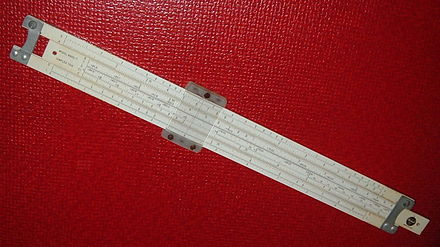
\includegraphics[width=\linewidth]{images/fig-side-rule.jpg}
\end{image}%
\tcblower
\end{figureptx}%
\end{sectionptx}
\end{chapterptx}
 %
%
\typeout{************************************************}
\typeout{Chapter 39 Posets and Lattices}
\typeout{************************************************}
%
\begin{chapterptx}{Posets and Lattices}{}{Posets and Lattices}{}{}{x:chapter:chapter_114}
\index{Poset}%
\index{Lattice}%
%
%
\typeout{************************************************}
\typeout{Section 39.1 Reading Assignment}
\typeout{************************************************}
%
\begin{sectionptx}{Reading Assignment}{}{Reading Assignment}{}{}{x:section:reading-114}
Read Sections 13.1 and 13.2 of \emph{Applied Discrete Structures}. Partial orderings were introduced in Chapter 6 and you might want to review the definition before you start on Chapter 13. You might recall that partial orderings tend to compare certain pairs of elements in a poset according to some size, where size might not always mean size in the conventional sense.  In any case, if we take two elements from a poset, an upper bound is something in the poset that is comparably larger than them both.  A lower bound is defined similarly. In some cases, we can define binary operations (``join'' and ``meet'') based on this idea.  When we can, we get an algebraic structure called a \emph{lattice}.%
\begin{question}{Response Question.}{g:question:idm218229144368}%
Google “total ordering” and find out if a total ordering is a “partial ordering.”%
\end{question}
Also, turn in solutions to these exercises:%
%
%
\typeout{************************************************}
\typeout{Exercises 39.1 Exercises}
\typeout{************************************************}
%
\begin{exercises-subsection-numberless}{Exercises}{}{Exercises}{}{}{g:exercises:idm218229153056}
\begin{divisionexercise}{1}{}{}{g:exercise:idm218229154672}%
For the poset \((\mathbb{N},\leq )\), what are the greatest lower bound and least upper bound of two elements \(a\) and \(b\)? Are there least and\slash{}or greatest elements?%
\end{divisionexercise}%
\begin{divisionexercise}{2}{}{}{g:exercise:idm218229161248}%
Let \(L\) be the set of all propositions generated by \(p\) and \(q\).  What are the meet and join operations in this lattice under implication?   What are the maximum and minimum elements?%
\end{divisionexercise}%
\end{exercises-subsection-numberless}
\end{sectionptx}
%
%
\typeout{************************************************}
\typeout{Section 39.2 In-Class Exercises}
\typeout{************************************************}
%
\begin{sectionptx}{In-Class Exercises}{}{In-Class Exercises}{}{}{x:section:questions-114}
%
%
%
\typeout{************************************************}
\typeout{Exercises 39.2 Exercises}
\typeout{************************************************}
%
\begin{exercises-subsection-numberless}{Exercises}{}{Exercises}{}{}{g:exercises:idm218229175328}
\begin{divisionexercise}{1}{}{}{g:exercise:idm218229175072}%
Consider the poset \((D_{50},\mid)\), where \(D_{50} = \{1,2,5,10,25,50\}\).%
\begin{enumerate}[label=(\alph*)]
\item{}Find all lower bounds of 10 and 25.%
\item{}Find the greatest lower bound  of 10 and 25.%
\item{}Find all upper bounds of 10 and 25.%
\item{}Determine the least upper bound  of 10 and 25.%
\item{}Draw the Hasse diagram for \(D_{50}\) with respect to \(\mid\).%
\end{enumerate}
%
\end{divisionexercise}%
\begin{divisionexercise}{2}{}{}{g:exercise:idm218229196768}%
Demonstrate that the pentagon lattice is nondistributive.%
\end{divisionexercise}%
\begin{divisionexercise}{3}{}{}{g:exercise:idm218229198800}%
We naturally order the numbers in \(A_m = \{1, 2, . . . , m\}\) with ``less than or equal to,'' which is a partial ordering. We define an ordering, \(\preceq\)  on the elements of \(A_m \times  A_n\) by%
\begin{equation*}
(a, b) \preceq  (a', b') \Leftrightarrow a \leq  a' \textrm{ and } b \leq  b'
\end{equation*}
%
\begin{enumerate}[label=(\alph*)]
\item{}Prove that \(\preceq\) is a partial ordering on \(A_m \times  A_n\).%
\item{}Draw the ordering diagrams for \(\preceq\) on \(A_2 \times  A_2\), \(A_2\times  A_3\), and \(A_3 \times  A_3\).%
\item{}In general, how does one determine the least upper bound  and greatest lower bound of two elements of \(A_m \times  A_n\), \((a, b)\) and \((a',b')\)?%
\item{}Are there least and\slash{}or greatest elements in \(A_m \times  A_n\)?%
\end{enumerate}
%
\end{divisionexercise}%
\begin{divisionexercise}{4}{}{}{g:exercise:idm218229261072}%
The last question you answered with the readings for this class is actually not very precise.  For example,  is it true that  \(p \Rightarrow p\land(p \lor q)\) or  \(p\land(p \lor q) \Rightarrow p\), or are both true?  If both are true, what does that say about the relation \(\Rightarrow\)?   This would present a problem, but it can be fixed by considering the elements of our poset to be equivalence classes.  What would be the equivalence classes?%
\end{divisionexercise}%
\end{exercises-subsection-numberless}
\end{sectionptx}
%
%
\typeout{************************************************}
\typeout{Section 39.3 Nondistributive lattices}
\typeout{************************************************}
%
\begin{sectionptx}{Nondistributive lattices}{}{Nondistributive lattices}{}{}{x:section:handouts-114}
\index{Non-distributive lattices}%
Here are the fundamental nondistributive lattices.%
\begin{figureptx}{Nondistributive lattices, the pentagon and diamond lattices}{x:figure:fig-nondistributive-lattices}{}%
\begin{image}{0.25}{0.5}{0.25}%
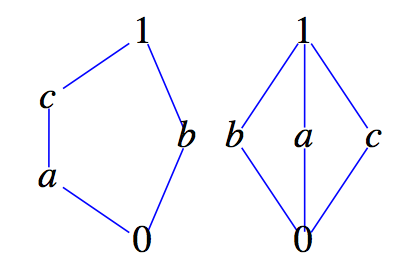
\includegraphics[width=\linewidth]{images/fig-nondistributive-lattices.png}
\end{image}%
\tcblower
\end{figureptx}%
\end{sectionptx}
\end{chapterptx}
 %
%
\typeout{************************************************}
\typeout{Chapter 40 Boolean Algebras}
\typeout{************************************************}
%
\begin{chapterptx}{Boolean Algebras}{}{Boolean Algebras}{}{}{x:chapter:chapter_115}
\index{Boolean Algebras}%
%
%
\typeout{************************************************}
\typeout{Section 40.1 Reading Assignment}
\typeout{************************************************}
%
\begin{sectionptx}{Reading Assignment}{}{Reading Assignment}{}{}{x:section:reading-115}
Read Section 13.3 of \emph{Applied Discrete Structures}.  In this section we further restrict our attention to lattices that have the algebraic properties that are required of a Boolean Algebra. Propositional logic that we saw in Chapter 3 is prime model for what Boolean Algebra is like, but there several other concrete Boolean Algebras that we will consider.%
\begin{question}{Response Question.}{g:question:idm218229294192}%
Why can't a lattice with three elements, a mininum element, a maximum element and third element between them be a boolean algebra?%
\end{question}
Also, turn in solutions to these exercises:%
\begin{itemize}[label=\textbullet]
\item{}Let \(D_n\) be the set of positive integers that divide evenly into \(n\).  List the elements of each of the sets \(D_{6}, D_{16}, D_{12}\textrm{, and }D_{30}\)%
\item{}What is the complement of a logical proposition in the Boolean algebra of logic?%
\end{itemize}
%
\end{sectionptx}
%
%
\typeout{************************************************}
\typeout{Section 40.2 In-Class Exercises}
\typeout{************************************************}
%
\begin{sectionptx}{In-Class Exercises}{}{In-Class Exercises}{}{}{x:section:questions-115}
\begin{figureptx}{Lattice of subgroups of \(\mathbb{Z}_{6}\)}{x:figure:fig-z6-subgroups}{}%
\begin{image}{0.3}{0.4}{0.3}%
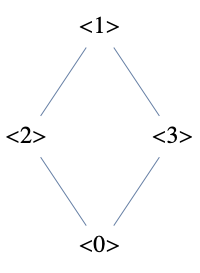
\includegraphics[width=\linewidth]{images/fig-z6-subgroups.png}
\end{image}%
\tcblower
\end{figureptx}%
%
\begin{enumerate}[label=\arabic*.]
\item{}Consider the lattices of divisors of 6, 12, 16, and 30, with the partial ordering ``divides''.%
\begin{enumerate}[label=(\alph*)]
\item{}Determine which elements of \(D_6\) have a complement.%
\item{}Determine which elements of \(D_{12}\) have a complement.%
\item{}Determine which elements of \(D_{16}\) have a complement.%
\item{}Determine which elements of \(D_{30}\) have a complement.%
\item{}Given that \(D_n\) is always a distributive lattice, for what values of \(n\) do you suppose \(D_n\) is a boolean algebra?%
\end{enumerate}
%
\item{}Recall that if \([G;*]\) is a finite group and \(a \in G\),  the cyclic subgroup generated by \(a\) is \(\langle a \rangle=\{a, a*a, a*a*a, \dots\}\), which is a finite set since you eventually get to the identity and can stop listing elements.  For example, if the group is \(\mathbb{Z}_{6}\), there are four different cyclic subgroups:  \(\langle 0 \rangle\), \(\langle 1 \rangle\), \(\langle 2 \rangle\), and \(\langle 3 \rangle\).  The other two elements of \(\mathbb{Z}_{6}\), 4 and 5 generate subgroups that are equal to the subgroups generated by 2 and 1, respectively.  The Hasse diagram for this set of subgroups with \(\subseteq\) is \hyperref[x:figure:fig-z6-subgroups]{Figure~{\xreffont\ref{x:figure:fig-z6-subgroups}}}%
\par
%
\begin{enumerate}
\item{}List the distinct cyclic subgroups generated by elements of \(\mathbb{Z}_{12}\). The set of subgroups you've found is a lattice with the partial ordering \(\subseteq\). Draw the Hasse diagram for this poset.%
\item{}Do the same with the cyclic subgroups generated by elements of \(\mathbb{Z}_{16}\).%
\item{}Do the same with the cyclic subgroups generated by elements of \(\mathbb{Z}_{30}\).%
\item{}Any general observations from the three cases?%
\end{enumerate}
%
\end{enumerate}
%
\end{sectionptx}
\end{chapterptx}
 %
%
\typeout{************************************************}
\typeout{Chapter 41 Atoms and Tuples of Bits}
\typeout{************************************************}
%
\begin{chapterptx}{Atoms and Tuples of Bits}{}{Atoms and Tuples of Bits}{}{}{x:chapter:chapter_116}
\index{Atoms and Tuples of Bits}%
%
%
\typeout{************************************************}
\typeout{Section 41.1 Reading Assignment}
\typeout{************************************************}
%
\begin{sectionptx}{Reading Assignment}{}{Reading Assignment}{}{}{x:section:reading-116}
Read Sections 13.4 and 13.5 of \emph{Applied Discrete Structures}. For any positive integer, \(n\), the number of different groups of order  \(n\) can vary quite a bit. In contrast, the number of Boolean Algebras of order  \(n\) is either zero or one. In these two sections, you will see why.%
\begin{question}{Response Question.}{g:question:idm218229433152}%
Consider the lattice of real numbers in the interval \([0,1]\) with the relation \(\leq\).  Does this lattice have any atoms?%
\end{question}
Also, turn in solutions to these exercises:%
\begin{itemize}[label=\textbullet]
\item{}What are the atoms of the lattice of subsets of \(\{1, 2, 3, 4, 5, 6, 7\}\)  generated by the two sets \(A_1=\{1,3,5,7\}\) and \(A_2=\{1,2,3,5\}\) with the partial ordering \(\subseteq\)?%
\item{}What are the atoms of the lattice of positive integers with the relation ``divides?''%
\end{itemize}
%
\end{sectionptx}
%
%
\typeout{************************************************}
\typeout{Section 41.2 In-Class Exercises}
\typeout{************************************************}
%
\begin{sectionptx}{In-Class Exercises}{}{In-Class Exercises}{}{}{x:section:questions-116}
%
\begin{enumerate}[label=\arabic*.]
\item{}%
\begin{enumerate}[label=(\alph*)]
\item{}There are many different, yet isomorphic, Boolean algebras with two elements. Describe one such Boolean algebra that is derived from a power set, \(\mathcal{P}(A)\), under \(\subseteq\). Describe a second that is described from \(D_n\), for some \(n \in  P\), under ``divides.''%
\item{}Since the elements of a two-element Boolean algebra must be the greatest and least elements, 1 and 0, the tables for the operations on \(\{0, 1\}\) are determined by the Boolean algebra laws. Write out the operation tables for \([\{0, 1\}; \lor , \land, -]\).%
\end{enumerate}
%
\item{}Consider the Boolean algebra \(\mathcal{B} = [B_2^6 ; \lor, \land, \- ]\), and let \(E_6\) be the set of bit strings of length six having an even number of 1's.  Is \(E_6\) closed with respect to the operations of \(\mathcal{B}\).%
\item{}Give an example of a Boolean algebra of order 16 whose elements are certain subsets of the set \(\{1, 2, 3, 4, 5, 6, 7\}\), the minimum element is the empty set, and the maximum element is \(\{1, 2, 3, 4, 5, 6, 7\}\).%
\item{}Give an example of a Boolean algebra of order 16 whose elements are a certain set of bit strings of the set \(B_2^7\), whose minimum element is \(0000000\), and whose maximum element is \(1111111\).%
\end{enumerate}
%
\end{sectionptx}
\end{chapterptx}
 %
%
\typeout{************************************************}
\typeout{Chapter 42 Cyclic Groups}
\typeout{************************************************}
%
\begin{chapterptx}{Cyclic Groups}{}{Cyclic Groups}{}{}{x:chapter:chapter_117}
\index{}%
%
%
\typeout{************************************************}
\typeout{Section 42.1 Reading Assignment}
\typeout{************************************************}
%
\begin{sectionptx}{Reading Assignment}{}{Reading Assignment}{}{}{x:section:reading-117}
Read Sections 15.1 of \emph{Applied Discrete Structures}. Some groups have the property that they are formed as a cyclic subgroup of one of its elements.  When this is the case, the group itself has a particularly simple form, which we examine in this section.%
\begin{question}{Response Question.}{g:question:idm218229544272}%
Google ``Chinese Remainder Theorem''. Why does the theorem have this name?%
\end{question}
Also, turn in solutions to these exercises:%
\begin{itemize}[label=\textbullet]
\item{}List all of the distinct cyclic subgroups of the cyclic group \(\mathbb{Z}_{15}\).  Explain why this list is actually a list of \emph{all} of the subgroups of \(\mathbb{Z}_{15}\).%
\item{}What are the generators of the multiplicative group \(\{5^k \mid k\in \mathbb{Z}\}\)?%
\end{itemize}
%
\end{sectionptx}
%
%
\typeout{************************************************}
\typeout{Section 42.2 In-Class Exercises}
\typeout{************************************************}
%
\begin{sectionptx}{In-Class Exercises}{}{In-Class Exercises}{}{}{x:section:questions-117}
%
\begin{enumerate}[label=\arabic*.]
\item{}What are the generators of the group \(\mathbb{Z}_{15}\)?  What relationship do these numbers have with the modulus, 15?%
\item{}Suppose \([G;*]\) is a cyclic group with generator \(g\). If you build a graph of with vertices from the elements of \(G\) and edge set \(E= \{(a, g*a) \mid a\in G\}\), what would the graph look like?  If \(G\) is a group of even order, what would a graph with edge set \(E'= \{(a, g^2*a) \mid a\in G\}\) look like?%
\item{}The function \(f: \mathbb{Z}_{77} \rightarrow \mathbb{Z}_7\times \mathbb{Z}_{11}\) defined by \(f(a)= (a mod 7, a mod 11)\) is an isomorphism.  Suppose you are given some elements in \(\mathbb{Z}_{77}\) and you want there sum (mod 77).  Furthermore, suppose you mapped these numbers, using \(f\), to \(\mathbb{Z}_7\times \mathbb{Z}_{11}\) and there sum in the direct product was \((1,6)\).  What is the sum in \(\mathbb{Z}_{77}\)?%
\end{enumerate}
%
\end{sectionptx}
\end{chapterptx}
 %
%
\typeout{************************************************}
\typeout{Chapter 43 Cosets}
\typeout{************************************************}
%
\begin{chapterptx}{Cosets}{}{Cosets}{}{}{x:chapter:chapter_118}
\index{}%
%
%
\typeout{************************************************}
\typeout{Section 43.1 Reading Assignment}
\typeout{************************************************}
%
\begin{sectionptx}{Reading Assignment}{}{Reading Assignment}{}{}{x:section:reading-118}
Read Section 15.2 of \emph{Applied Discrete Structures}. If you get confused in this section, think about the partition of the integers into even integers and odd integers.  There is a consistency in doing arithmetic on the integers where, for example, any time you add an even integer and an odd integer, you get an odd integer.  So \(\textrm{even} + \textrm{odd} = \textrm{even}\).  This is coset addition!  For any group, the only way something like this can work is when the partition is into cosets, which is why we start by defining this set of subsets of a group.%
\begin{question}{Response Question.}{g:question:idm218227603312}%
How did Galois die, and why am I asking you this?%
\end{question}
Also, turn in solutions to these exercises:%
\begin{enumerate}[label=\arabic*.]
\item{}What does Lagrange's Theorem say about the possible subgroups of a group of order 12?%
\item{}Let \(H\) be the subgroup \(\{0,25,50,75\}\) of the additive group \(\mathbb{Z}_{100}\). How many distinct left cosets are there of \(H\)?  What coset contains the number 42? List its elements.%
\end{enumerate}
%
\end{sectionptx}
%
%
\typeout{************************************************}
\typeout{Section 43.2 In-Class Exercises}
\typeout{************************************************}
%
\begin{sectionptx}{In-Class Exercises}{}{In-Class Exercises}{}{}{x:section:questions-118}
%
\begin{enumerate}[label=\arabic*.]
\item{}List the distinct left cosets of the cyclic subgroup of \(U_{13}\) generated by 3. To what other group is the factor group of these cosets isomorphic?%
\item{}For each group and subgroup, to what simpler group is  \(G/H\) isomorphic?  Draw a picture of the groups and their cosets.%
\begin{enumerate}[label=(\alph*)]
\item{}\(G= \mathbb{R}^2\)  and  \(H = \{(a,a) \mid a\in\mathbb{R}\}\)%
\item{}\(G = \mathbb{Z}_2^3\)  and  \(H = \langle 111 \rangle\).  In this group, write triples as bit strings of length 3.%
\end{enumerate}
%
\item{}Consider the subgroup \(C = \{00000, 01101, 11110, 10011\}\) of the group \(S=\mathbb{Z}_2^5\). Suppose your answer to a multiple choice question with four possible responses is stored in five bits of computer memory using one of the four elements of  \(C\).  Now suppose the computer is hacked but we know that no more than one of the five bits in your response has been changed.  Can your response be recovered?%
\end{enumerate}
%
\end{sectionptx}
\end{chapterptx}
 %
%
\typeout{************************************************}
\typeout{Chapter 44 Permutation Groups, Part 1}
\typeout{************************************************}
%
\begin{chapterptx}{Permutation Groups, Part 1}{}{Permutation Groups, Part 1}{}{}{x:chapter:chapter_119}
\index{}%
%
%
\typeout{************************************************}
\typeout{Section 44.1 Reading Assignment}
\typeout{************************************************}
%
\begin{sectionptx}{Reading Assignment}{}{Reading Assignment}{}{}{x:section:reading-119}
Read the first two subsections of Section 15.3 of \emph{Applied Discrete Structures}, stopping when you get to  Subsection 15.3.3. Our focus in this section is on whole sets of functions, but we also consider convenient ways to represent individual functions.  In most cases, you'll find that cycle notation is probably the best option, even though it might look strange at first.%
\begin{question}{Response Question.}{g:question:idm218227921856}%
Joseph-Louis Lagrange (1736-1813) first thought of permutations as functions from a set to itself. However, he didn't invent cycle notation.  Who did that?%
\end{question}
Also, turn in solutions to these exercises:%
\begin{enumerate}[label=\arabic*]
\item{}Write the following elements of \(S_5\) as a product of disjoint cycles.%
\begin{multicols}{2}
\begin{enumerate}[label=(\alph*)]
\item{}\(\displaystyle \alpha=\left(
\begin{array}{ccccc}
1 & 2 & 3 & 4 & 5 \\
2 & 4 & 1 & 5 & 3 \\
\end{array}
\right)\)%
\item{}\(\displaystyle \beta=\left(
\begin{array}{ccccc}
1 & 2 & 3 & 4 & 5 \\
4 & 2 & 5 & 1 & 3 \\
\end{array}
\right)\)%
\end{enumerate}
\end{multicols}
%
\item{}Compute the following using the values of \(\alpha\) and \(\beta\) above.  Write your answer as a product of disjoint cycles.%
\begin{multicols}{2}
\begin{enumerate}[label=(\alph*)]
\item{}\(\displaystyle \alpha \circ \beta\)%
\item{}\(\displaystyle \beta \circ \alpha\)%
\item{}\(\displaystyle \alpha^{-1}\)%
\item{}\(\displaystyle \beta^{-1}\)%
\end{enumerate}
\end{multicols}
%
\end{enumerate}
%
\end{sectionptx}
%
%
\typeout{************************************************}
\typeout{Section 44.2 In-Class Exercises}
\typeout{************************************************}
%
\begin{sectionptx}{In-Class Exercises}{}{In-Class Exercises}{}{}{x:section:questions-119}
There are advantages to cycle notation.  One is that the order of an element can be determined by its cycle structure.%
\begin{enumerate}[label=\arabic*.]
\item{}What are the orders of the following permutations?%
\begin{multicols}{3}
\begin{enumerate}[label=(\alph*)]
\item{}\(\displaystyle (1,2,3)\)%
\item{}\(\displaystyle (1,2,3,4)\)%
\item{}\(\displaystyle (1,2,3)(4,5)\)%
\item{}\(\displaystyle (1,2,3)(4,5,6)\)%
\item{}\(\displaystyle (1,2,3,4)(5,6)\)%
\item{}\(\displaystyle (1,6)(1,5)(1,4)(1,3)(1,2)\)%
\end{enumerate}
\end{multicols}
%
\item{}Based on the result in the previous problem, predict the orders of the following permutations without actually computing their powers.%
\begin{multicols}{3}
\begin{enumerate}[label=(\alph*)]
\item{}\(\displaystyle (1,2,3,4,5,6,7)\)%
\item{}\(\displaystyle (1,2,3,4)(5,6,7,8)\)%
\item{}\(\displaystyle (1,2,3,4)(5,6,7)\)%
\end{enumerate}
\end{multicols}
%
\item{}Among all permutations in \(S_{10}\), what is their largest order?  How about \(S_{11}\)?%
\item{}Prove that if \(\sigma\) and \(\phi\) are permutations, then the order of \(\phi \circ \sigma \circ \phi^{-1}\) is equal to the order of \(\sigma\).%
\end{enumerate}
%
\end{sectionptx}
%
%
\typeout{************************************************}
\typeout{Section 44.3 The order of a group element}
\typeout{************************************************}
%
\begin{sectionptx}{The order of a group element}{}{The order of a group element}{}{}{x:section:handouts-119}
Here is a reminder of the definition of \emph{order}.%
\begin{definition}{Order of a Group Element.}{x:definition:def-order-of-element}%
\index{Order of a Group Element}%
\label{g:notation:idm218228216272}%
The order of an element \(a\) of group \(G\) is the number of elements in the cyclic subgroup of \(G\) generated by \(a\). The order of \(a\) is denoted \(ord(a)\).%
\end{definition}
\end{sectionptx}
\end{chapterptx}
 %
%
\typeout{************************************************}
\typeout{Chapter 45 Permutation Groups, Part 2}
\typeout{************************************************}
%
\begin{chapterptx}{Permutation Groups, Part 2}{}{Permutation Groups, Part 2}{}{}{x:chapter:chapter_120}
\index{}%
%
%
\typeout{************************************************}
\typeout{Section 45.1 Reading Assignment}
\typeout{************************************************}
%
\begin{sectionptx}{Reading Assignment}{}{Reading Assignment}{}{}{x:section:reading-120}
Read the rest of  Section 15.3 of \emph{Applied Discrete Structures}. The family \(S_n\) of symmetric groups is extremely important in group theory, particularly when it comes to doing computations.   There is a theorem called Cayley's Theorem that essentially says that \emph{every} group is  subgroup of some symmetric group.  This means that if you intend to do group computations, it's natural to implement the work in terms of permutations.%
\begin{question}{Response Question.}{g:question:idm218228271904}%
How is Rubik's cube related to permutation groups?%
\end{question}
Also, turn in solutions to these exercises:%
\begin{itemize}[label=\textbullet]
\item{}Based on \emph{Lagrange's Theorem}, what are the possible orders of subgroups of the group \(S_4\)?%
\item{}The \emph{shape} of a permutation, \(\sigma\) in \(S_n\) is the sequence of lengths of the cycles in the representaion of \(\sigma\) as a product of disjoint cycles. The lengths are written in descending order.  For example, if \(\sigma = (1,3,4)(8,11)(2,5,6,7)(9,10)(12) \in S_{12}\), then its shape is  4,3,2,2,1.  List all possible shapes of elements in \(S_4\).%
\end{itemize}
%
\end{sectionptx}
%
%
\typeout{************************************************}
\typeout{Section 45.2 In-Class Exercises}
\typeout{************************************************}
%
\begin{sectionptx}{In-Class Exercises}{}{In-Class Exercises}{}{}{x:section:questions-120}
%
\begin{enumerate}[label=\arabic*.]
\item{}Prove that \(H =\{\sigma \in S_5 \mid \sigma(5)=5 \}\) is a subgroup of \(S_5\).  How many elements does \(H\) have?%
\item{}Given a graph with vertex set \(\{1, 2, 3, 4, 5\}\), the group of automorphisms of that graph will be a subgroup of the group  \(S_4\). For each of the following subgroups of \(S_5\), draw a graph (directed or undirected) that has that subgroup as its automorphism group.%
\begin{enumerate}[label=(\alph*)]
\item{}\(\displaystyle \{i\}\)%
\item{}The cyclic subgroup generated by \((1,2)\)%
\item{}The cyclic subgroup generated by \((1,2,3,4,5)\)%
\item{}\(\displaystyle \{\sigma \in S_5 \mid \sigma(5)=5  \}\)%
\end{enumerate}
%
\item{}There are subgroups of \(S_n\) that are not the automorphism group of of any graph with \(n\) vertices.  Illustrate this fact by showing that it is true for \(S_4\).  However, for any such subgroup, \(H\), there are graphs with a larger number of vertices that have automorphism groups that are isomorphic to \(H\). Illustrate this fact with the subgroup you identified in \(S_4\).%
\end{enumerate}
%
\end{sectionptx}
\end{chapterptx}
 %
%
\typeout{************************************************}
\typeout{Chapter 46 Algebraic Coding, Part 1}
\typeout{************************************************}
%
\begin{chapterptx}{Algebraic Coding, Part 1}{}{Algebraic Coding, Part 1}{}{}{x:chapter:chapter_121}
\index{}%
%
%
\typeout{************************************************}
\typeout{Section 46.1 Reading Assignment}
\typeout{************************************************}
%
\begin{sectionptx}{Reading Assignment}{}{Reading Assignment}{}{}{x:section:reading-121}
Read the definition of \emph{Homomorphism} in Section 15.4. Then read Section 15.5 of \emph{Applied Discrete Structures} up to, but not including, Subsection 15.5.2 Error Correction. After outlining the objectives behind coding theory we first consider how to effectively detect transmission errors.%
\begin{question}{Response Question.}{g:question:idm218228477424}%
If you measure the distance between elements of a set, \(S\), with a function \(d: S\times S \rightarrow \mathbb{R}\), what general distance properties would you expect of this function?%
\end{question}
Also, turn in solutions to these exercises:%
\begin{enumerate}[label=\arabic*.]
\item{}\emph{Interogating a Liar}.  I'm a liar, but not a big one.  In my responses to your yes\slash{}no questions, I promise not to lie more than one time.  I'm thinking of a number, either 0 or 1.  How many yes\slash{}no questions do you need to ask in order to find out my number? Explain your logic.%
\item{}The \emph{Hamming Distance}, \(d_H\), between two strings of bits with the same length is the number positions within the two strings where the strings differ.  For instance, \(d_H(11101,10100)=2\) because the two strings differ in positions 2 and 5.  What is the minimal Hamming distance between any two strings in the set%
\begin{equation*}
C =\{00000,11011,11100,00111\}?
\end{equation*}
%
\end{enumerate}
%
\end{sectionptx}
%
%
\typeout{************************************************}
\typeout{Section 46.2 In-Class Exercises}
\typeout{************************************************}
%
\begin{sectionptx}{In-Class Exercises}{}{In-Class Exercises}{}{}{x:section:questions-121}
%
\begin{enumerate}[label=\arabic*.]
\item{}Suppose a two bit message is encoded into a five bit message using the function \(e(b_{1}b_{2})=b_{1}b_{1}(b_{1}+_2 b_{2})b_{2}b_{2}\).  What matrix, \(G\), has the property that \(e(b_{1}b_{2})=(b_{1} b_{2}) G\)?%
\item{}Define the two functions  \(g:\mathbb{Z}_2{}^3\rightarrow  \mathbb{Z}_2{}^4\)  and \(p:\mathbb{Z}_2{}^4\to \mathbb{Z}_2\) by \(g(a_1,a_2,a_3) = (a_1,a_2,a_3 ,a_1+_2 a_2+_2a_3)\), and \(p(b_1,b_2,b_3,b_4)=b_1+b_2+b_3+b_4\).%
\begin{enumerate}[label=(\alph*)]
\item{}The values of \(g(a_1,a_2,a_3)\) and \(p(b_1,b_2,b_3,b_4)\) can be computed as matrix products.  Determine the matrices.%
\item{}Describe the function \(p \circ g\). Is it a homomorphism?%
\end{enumerate}
%
\item{}Suppose we were to send three bits across a binary symmetric channel by first encoding the bits using the function \(g\) from the previous problem, producing a sequence of four bits.   After receiving the four bits, the person at the receiving end applies the function \(p\) to those bits.   What can we derivive form the output of \(p\)?%
\item{}\emph{Linear Codes}.  Let \(m\) and \(n\) be positive integers.  Suppose that \(G\) is an \(m \times n\) matrix of zeros and ones.  Then we can can define a function \(e:\mathbb{Z}_2^m \rightarrow \mathbb{Z}_2^n\) by \(e(a)=a G\) where we take \(a \in \mathbb{Z}_2^m\) to be a 	\(1\times m\) matrix and we perform mod 2 arithmetic in computing the product \(a G\).  Prove that \(e\) is a homomorphism.%
\end{enumerate}
%
\end{sectionptx}
\end{chapterptx}
 %
%
\typeout{************************************************}
\typeout{Chapter 47 Algebraic Coding, Part 2}
\typeout{************************************************}
%
\begin{chapterptx}{Algebraic Coding, Part 2}{}{Algebraic Coding, Part 2}{}{}{x:chapter:chapter_122}
\index{}%
%
%
\typeout{************************************************}
\typeout{Section 47.1 Reading Assignment}
\typeout{************************************************}
%
\begin{sectionptx}{Reading Assignment}{}{Reading Assignment}{}{}{x:section:reading-122}
Read the rest of  Section 15.5 of \emph{Applied Discrete Structures}.  We consider how to correct transmission errors by using redundant information in a coded message.  This avoids having to ask for a message to be resent from the sender.%
\begin{question}{Response Question.}{g:question:idm218183626176}%
Who was Claude Shannon and what is his connection with coding theory?%
\end{question}
Also, turn in solutions to these exercises:%
\begin{enumerate}[label=\arabic*.]
\item{}What is the minimum Hamming distance between code words in the set \(\{11100,00111,10001,01010\}\)? Without doing any calculation, how can you tell%
\begin{equation*}
\{11100,00111,10001,01010\}
\end{equation*}
cannot be the code words of a linear code?%
\item{}I'm a liar, but not a big one.  In my responses to your yes\slash{}no questions, I promise not to lie more than one time. My favorite number is 0, 1, 2, or 3.  How many yes\slash{}no questions do you need to ask in order to figure it out? You need to submit all of your questions to me without waiting for my answers. (thanks to Daniel Glasscock for this problem)%
\end{enumerate}
%
\end{sectionptx}
%
%
\typeout{************************************************}
\typeout{Section 47.2 In-Class Exercises}
\typeout{************************************************}
%
\begin{sectionptx}{In-Class Exercises}{}{In-Class Exercises}{}{}{x:section:questions-122}
%
\begin{enumerate}[label=\arabic*.]
\item{}Suppose a two bit message is encoded into a five bit message using the function \(e(b_{1}b_{2})=b_{1}b_{1}(b_{1}+_2 b_{2})b_{2}b_{2}\).  Determine a matrix \(P\) such that if a two bit message, \(b = b_{1}b_{2}\), is encoded and \(e(b)\) transmitted, then any single bit error in the received string \(c=c_{1}c_{2}c_{3}c_{4}c_{5}\) can be identified by whether \(c P\) is the zero vector or not.%
\item{}Consider the  linear code defined by the generator matrix%
\begin{equation*}
G=\left(
\begin{array}{cccc}
1 & 0 & 1 & 0 \\
0 & 1 & 1 & 1 \\
\end{array}
\right)
\end{equation*}
%
\par
%
\begin{enumerate}[label=(\alph*)]
\item{}What size blocks does this code encode and what is the length of the code words?%
\item{}What are the code words for this code?%
\item{}With this code, can you detect single bit errors?  Can you correct all, some, or no single bit errors?%
\end{enumerate}
%
\item{}\index{Rectangular Code}To build a \terminology{rectangular code}, you partition your message into blocks of length \(m\) and then factor \(m\) into \(k_1\cdot k_2\)  and arrange the bits in a  \(k_1 \times k_2\) rectangular array as in the figure below.  Then you add parity bits along the right side and bottom of the rows and columns.   The code word is then read row by row.%
\begin{equation*}
\begin{array}{cccccc}
\blacksquare  & \blacksquare  & \blacksquare  & \cdots  & \blacksquare  & \square  \\
\blacksquare  & \blacksquare  & \blacksquare  & \cdots  & \blacksquare  & \square  \\
\vdots  & \vdots  & \vdots  &   & \vdots  & \vdots  \\
\blacksquare  & \blacksquare  & \blacksquare  & \cdots  & \blacksquare  & \square  \\
\square  & \square  & \square  & \cdots  & \square  &   \\
\end{array}  \quad \begin{array}{c}
\textrm{      }\blacksquare  = \textrm{ message} \textrm{ bit} \\
\square  =\textrm{ parity} \textrm{ bit} \\
\end{array}
\end{equation*}
%
\par
For example, if \(m\) is 4, then our only choice is a 2 by 2 array.  The message 1101 would be encoded as%
\begin{equation*}
\begin{array}{cc|c}
1 & 1 & 0\\
0 & 1 & 1\\
\hline
1 & 0 &\\
\end{array}
\end{equation*}
and the code word is the string 11001110.%
\par
%
\begin{enumerate}[label=(\alph*)]
\item{}Suppose that you were sent four bit messages using this code and you received the following strings.  What were the messages, assuming no more than one error in the transmission of coded data?%
\begin{multicols}{3}
\begin{enumerate}[label=(\roman*)]
\item{}11011000%
\item{}01110010%
\item{}10001111%
\end{enumerate}
\end{multicols}
%
\item{}If you encoded \(n^2\) bits in this manner, what would be the rate of the code?%
\item{}Rectangular codes are linear codes.  For the 3 by 2 rectangular code, what are the generator and parity check matrices?%
\end{enumerate}
%
\item{}A code with minimum distance \(d\) is called \emph{perfect} if every string of bits is within Hamming distance \(r=\frac{d-1}{2}\) of some codeword. For such a code, the spheres of radius \(r\) around the codewords partition the set of all strings.  This is analogous to packing objects into a box with no wasted space.  Using just the number of bit strings of length \(n\) and the number of strings in a sphere of radius \(1\), for what values of \(n\) is it possible to find a perfect code of distance \(3\)?  You don't have to actually find the codes.%
\end{enumerate}
%
\end{sectionptx}
\end{chapterptx}
\end{partptx}
%
\backmatter%
%
\clearpage\phantomsection%
\addcontentsline{toc}{part}{Back Matter}%
%
%
\typeout{************************************************}
\typeout{References  References}
\typeout{************************************************}
%
\begin{references-chapter-numberless}{References}{}{References}{}{}{g:references:idm218228661328}
\index{References}%
%% If this is a top-level references
%%   you can replace with "thebibliography" environment
\begin{referencelist}
\bibitem[1]{x:biblio:biblio-bogart-2017}\hypertarget{x:biblio:biblio-bogart-2017}{}Bogart, Kenneth P., \textit{Combinatorics Through Guided Discovery}, \href{http://bogart.openmathbooks.org}{http:\slash{}\slash{}bogart.openmathbooks.org}
\bibitem[2]{x:biblio:biblio-doerr-2019}\hypertarget{x:biblio:biblio-doerr-2019}{}Doerr, A, and K. Levasseur, \textit{Applied Discrete Structures}, \href{http://discretemath.org}{http:\slash{}\slash{}discretemath.org}
\bibitem[3]{x:biblio:biblio-levin-2020}\hypertarget{x:biblio:biblio-levin-2020}{}Levin, Oscar, \textit{Discrete Mathematics: An Open Introduction}, \href{http://discrete.openmathbooks.org}{http:\slash{}\slash{}discrete.openmathbooks.org}, \par%
A one semester open source text with some nice features%

\bibitem[4]{x:biblio:biblio-pengelley}\hypertarget{x:biblio:biblio-pengelley}{}David Pengelley, \textit{From Lecture to Active Learning: Rewards for All, and Is It Really So Difficult?}, The College Math Journal, January 2020, \textbf{51} no.\@\,1, 13\textendash{}24, doi.org\slash{}10.1080\slash{}07468342.2020.1680228\par%
The idea of teaching in an active learning environment had been on my radar for a while and I'd experimented with some aspects of the format. This article was the final impetus for launching this project.%

\end{referencelist}
\end{references-chapter-numberless}
%
%% The index is here, setup is all in preamble
%% Index locators are cross-references, so same font here
{\xreffont\printindex}
%
\end{document}